\Chapter{Detector Research, Development, Construction, and Commissioning}
\label{Ch4}

Research and development for the PROSPECT AD began in 2014.
The timeline of PROSPECT R\&D is shown in Table~\ref{tab:Prototypes}.
With the goals of maximizing the $^6$LiLS performance and background subtraction, as well as minimizing the dead volume and liquid degradation, the detector design was tested and demonstrated by multiple prototype detectors.

After two years of R\&D, the fabrication of the detector components and the $^6$LiLS were organized in different facilities that mainly included the Illinois Institute of Technology (IIT), Yale University (Yale), and Brookhaven National Laboratory (BNL).
Comprehensive quality control (QC) and quality assurance (QA) were included in fabrication procedures to ensure detector performance, especially detector stability and segment uniformity. 

During the detector R\&D, I co-led the efforts of design, fabrication, QC and QA of the optical grid components.
I also took significant role in the assembly of the PMT modules, the detector inner volume, as well as the detector commissioning at the HFIR facility.

This chapter briefly describes the prototype detectors of PROSPECT, and details the design and fabrication of the detector components. 
Descriptions of detector assembly and commissioning  are also included.

\FloatBarrier
\begin{sidewaystable}[!ht]
    \centering
    \caption[PROSPECT R\&D and construction phases]{PROSPECT R\&D and construction phases.}
    \begin{tabular}{p{4cm}lp{8cm}ll}
         \hline
		\hline
        Phase & Time & Goal & Location & Reference \\
        \hline
        0.1~liter prototype  & Aug. 2014 & DAQ, LS performance & Yale University &\\
        2~liter prototype   & Dec. 2014 to Mar. 2015 & Background survey, shielding & HFIR &\cite{bib:prospect_background}\\
        20~liter prototype   & Mar. 2015 to Aug. 2016 & Single segment performance & HFIR and Yale & \cite{bib:P20} \\
        50~liter prototype   & Jan. 2016 to Mar. 2019 & Two-segment event reconstruction, detector stability & Yale University & \cite{bib:P50} \\
        \hline
        Optical grid component fabrication & Nov. 2016 to Sept. 2017 & Component fabrication and optical measurements  & \cite{bib:prospect_og} \\  
        LS fabrication & Jan. 2017 to Oct. 2017 & LS production, $^6$Li loading, $^{227}$Ac loading & BNL & \cite{bib:lspaper} \\
        PMT module assembly & Sept. 2016 to Oct. 2017 & PMT delivery, test, module assembly & Yale & \\
        \hline
	   	Detector assembly & Oct. 2017 to Dec. 2017 & Detector assembly, electronic initial test & Yale & \cite{bib:prospect_nim, bib:prospect_og} \\       
       	Detector commissioning & Dec. 2017 to Mar. 2019 & LS filling, shielding assembly, calibration system assembly, detector initial commissioning & HFIR & \\ 
        \hline 
        Data acquisition & since Mar. 2018 & Data acquisition & HFIR & \cite{bib:P50} \\ 
        \hline
    \end{tabular}
        \label{tab:Prototypes}
\end{sidewaystable}
\FloatBarrier


\Section{Prototype Research}

In early R\&D phases, prototype detectors were assembled to develop and demonstrate a variety of designed detector features.
During this phase, many candidate materials were tested. 
The first PROSPECT prototype detector was built with a cylindrical test cell filled with 0.1~liter $^6$LiLS.
This prototype demonstrated the $n$-Li capture and PSD features of the $^6$LiLS.

From December 2014 to March 2015, a 2-liter prototype detector (PROSPECT-2) was deployed at the designed detector location in the HFIR facility building with a primary purpose of performing an on-site background survey.
As shown in Figure~\ref{fig:P2b}, this prototype was a single volume cylindrical detector surrounded by specular reflectors with two PMTs on its ends. 
By comparing the reactor-on and -off gamma and neutron detection rate, this prototype demonstrated a shielding strategy that could effectively eliminate reactor correlated gamma and $n$-Li capture events~\cite{bib:prospect_background}.

\begin{figure}[h!]
    \centering
    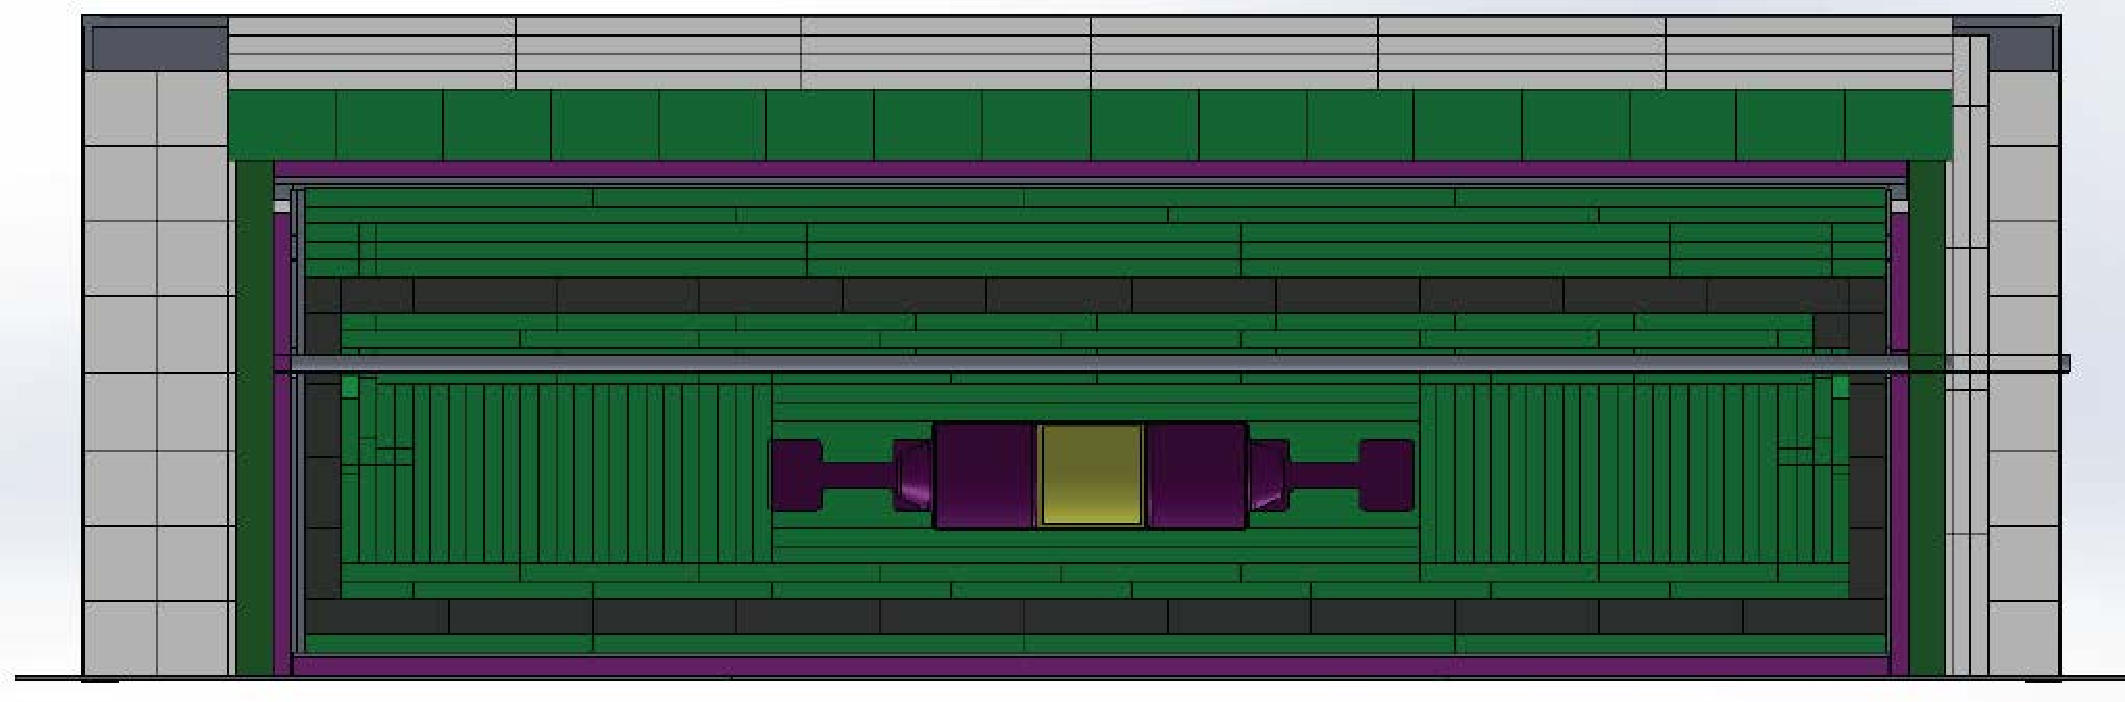
\includegraphics[width=0.8\textwidth]{Figures/P2B_Shield.pdf}
    \caption[A schematic of the 2-liter prototype with shielding]{PROSPECT-2 prototype installed at HFIR. 
    The 5” cylindrical LS detector (yellow), PMTs and HV bases (purple) are surrounded by 5\% borated polyethylene sheets (green), lead (dark grey), more 5\% borated polyethylene sheet, an Al containment box ( grey), 30\% borated
polyethylene sheet (purple), more 5\% borated polyethylene sheet, and polyethylene sheet (light grey).}
    \label{fig:P2b}
\end{figure}

Two 23-liter prototypes (PROSPECT-20)~\cite{bib:P20} were deployed at HFIR and Yale, respectively.
The goals of these two prototypes were to further characterize background, as well as study the scintillator performance and stability~\cite{bib:P20}.
Figure~\ref{fig:P20a} shows the design of the PROSPECT-20 detector. 
The dimensions of PROSPECT-20 prototype were similar to a single segment of the full PROSPECT AD.
PROSPECT-20 demonstrated the PSD performance, energy reconstruction, and position reconstruction with respect to gamma calibration sources deployed along with the detector.
Several candidate designs and materials for the PMT module were also tested in these prototype studies.
For instance, PROSPECT-20 first included and tested the utilization of specular reflectors and two-PMT readout to optimize the PSD performance and light collection of the detector.

\begin{figure}[h!]
    \centering
    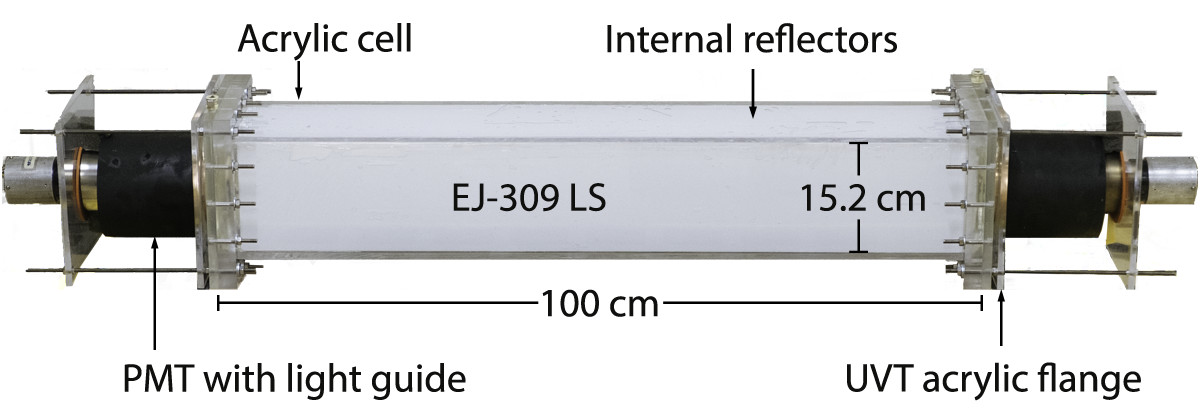
\includegraphics[width=0.8\textwidth]{Figures/P20_InternalReflectors.jpg}
    \caption[The schematic of the 23-liter prototype]{The schematic of the 23-liter prototype with labeled key components~\cite{bib:P20}.}
    \label{fig:P20a}
\end{figure}

A prototype containing 50~liters of $^6$LiLS (PROSPECT-50)~\cite{bib:P50} was assembled and tested at Yale to validate the product components for the final PROSPECT AD.
Figure~\ref{fig:P50x} shows the schematic of this prototype.
The PROSPECT-50 detector consisted of two segments whose dimensions are identical to the designed dimensions of the segments of the finalized detector.
The chemical compatibility of detector components, including PMT modules, optical grid, calibration system, and cables, were tested in direct contact with $^6$LiLS.
PROSPECT-50 also provides a parallel light yield stability monitor for the PROSPECT AD. 
Cosmogenic background, gamma, and neutron calibrations were measured with this 50~liter prototype.
These measurements led to the development of analysis packages for segment-based event reconstruction and validated the detector simulation through data to Monte-Carlo comparisons.

\begin{figure}[h!]
    \centering
    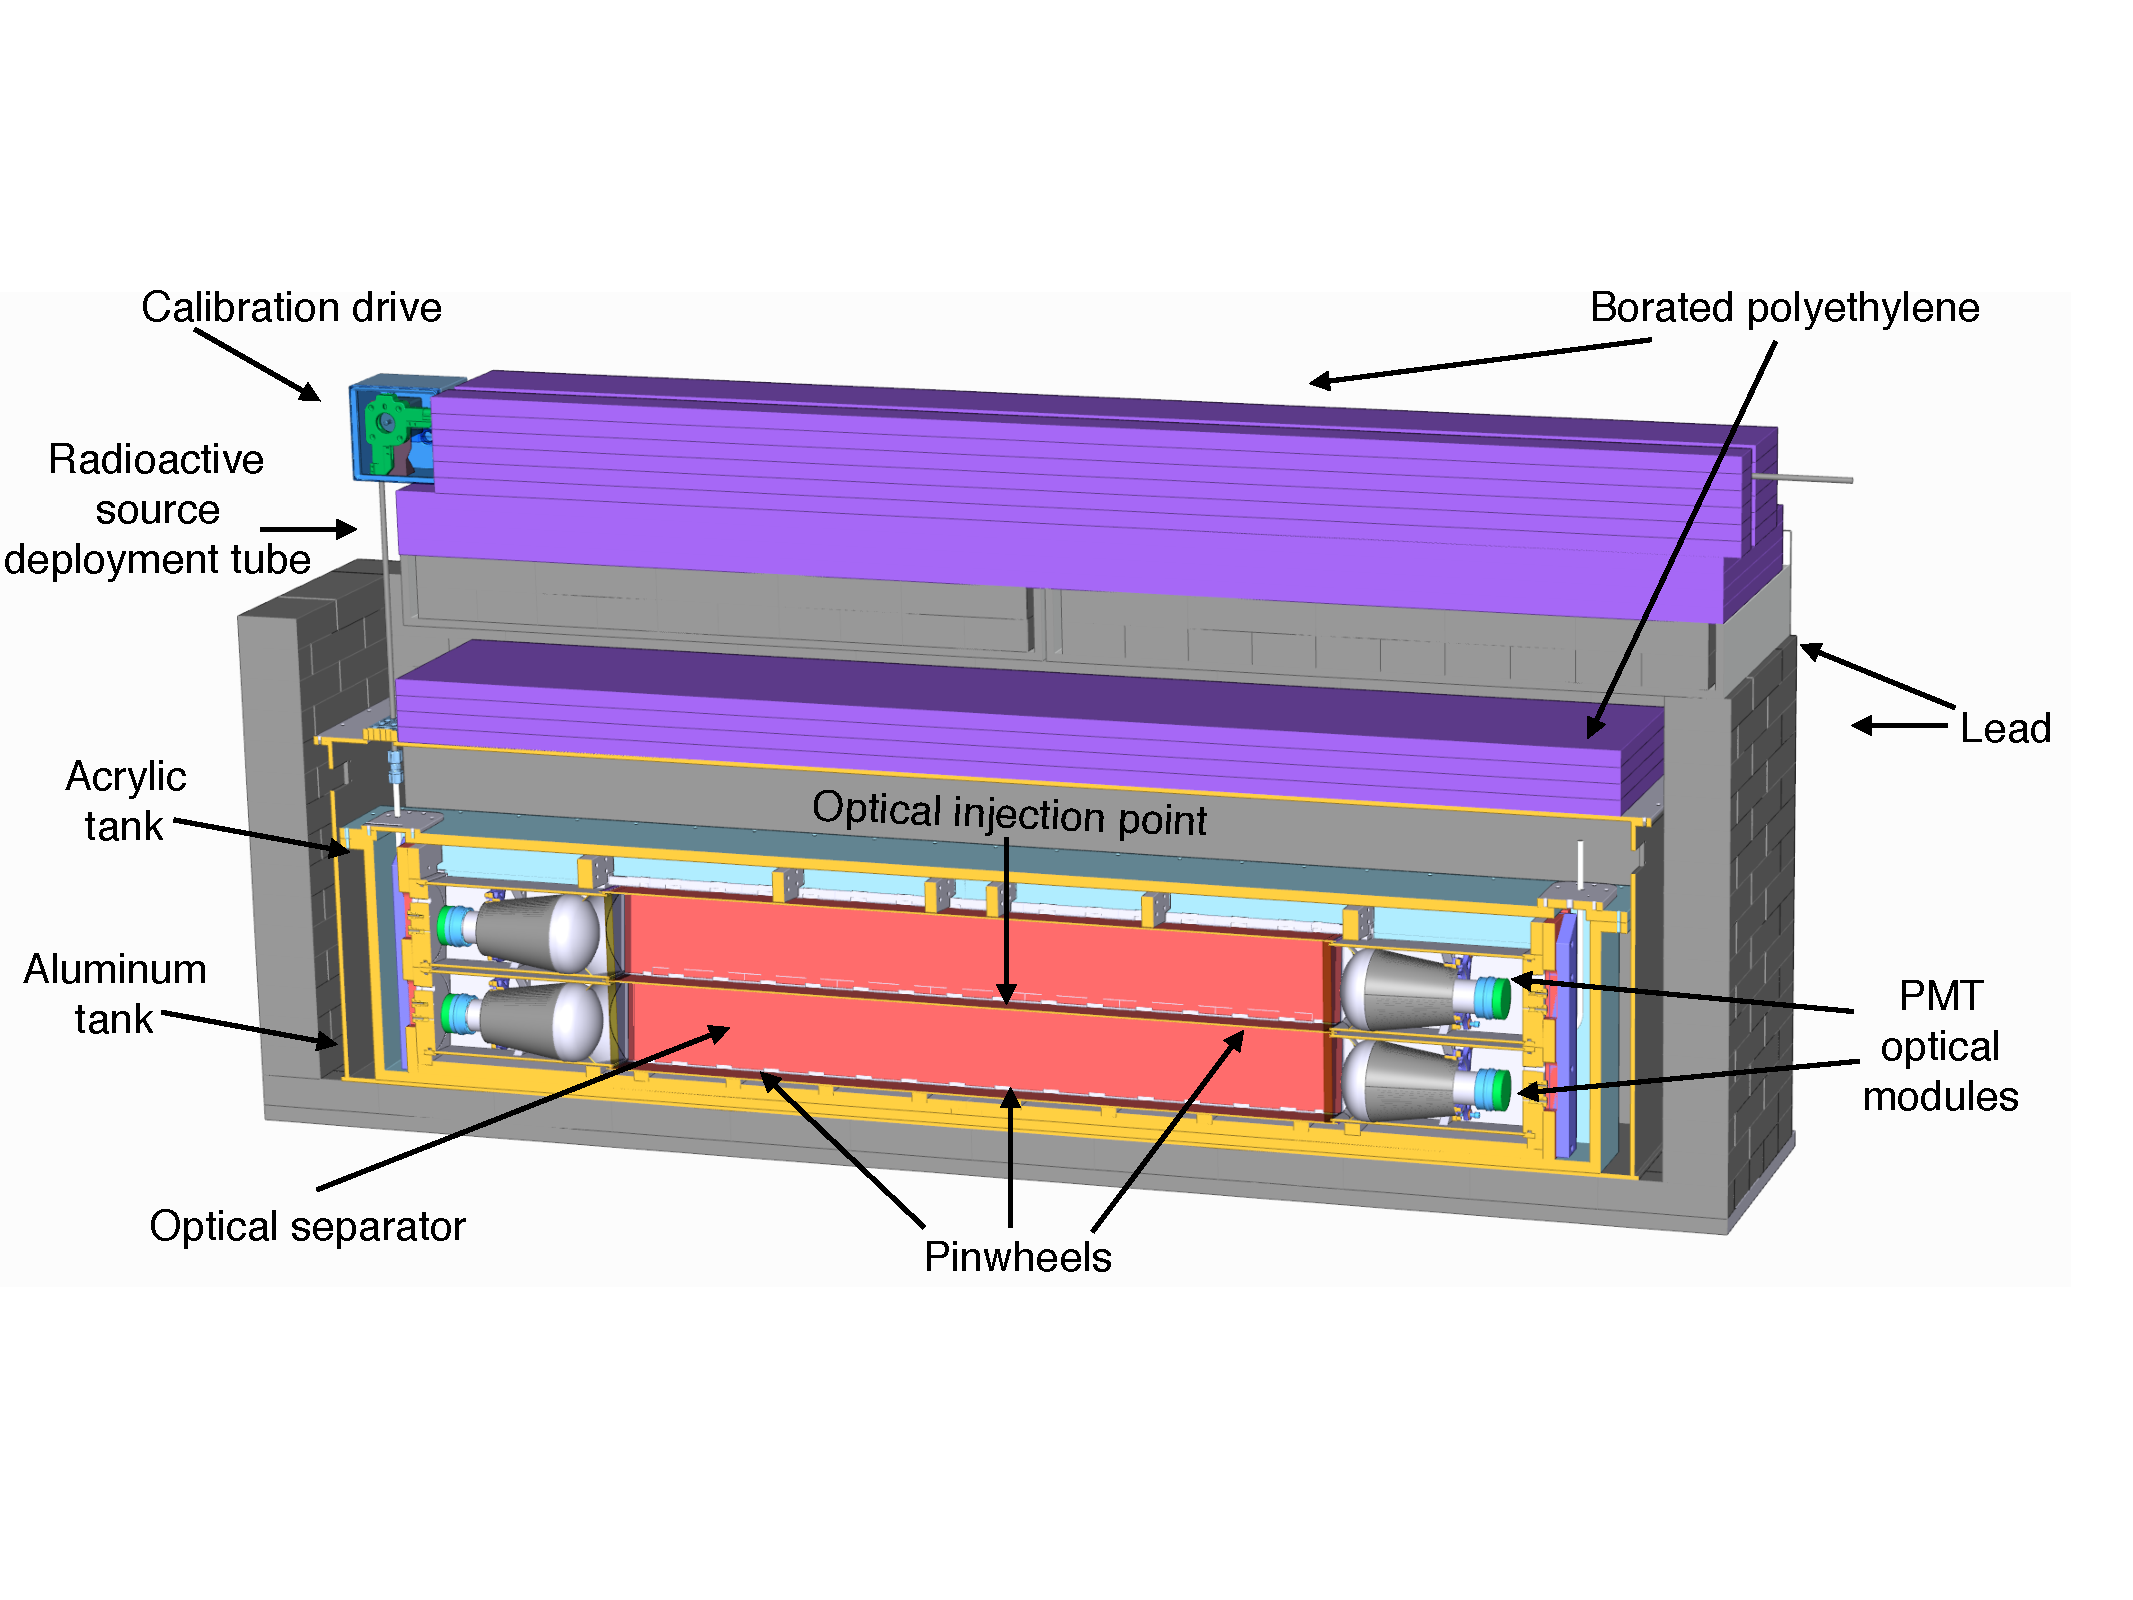
\includegraphics[width=0.8	\textwidth]{Figures/P50.pdf}
    \caption[A schematic of the 50-liter prototype]{A schematic of the PROSPECT-50 prototype with labeled key components~\cite{bib:P50}.}
    \label{fig:P50x}
\end{figure}

\Section{$^6$Li Loaded Liquid Scintillator}
\label{sec:LiLS}

$^6$LiLS is the target material of the PROSPECT AD.
The base scintillator, EJ-309, is a di-isopropyl naphthalene based liquid organic scintillator with 2,5-diphenyloxazole and 1,4-bis(2-methylstyryl) benzene dissolved as the wavelength shifter to cover the wavelength range of the PMT light collection in PROSPECT.
The $^6$Li isotope was loaded with the LiCl solution that dissolved in the base scintillator with an aqueous surfactant.
The $^6$LiCl solution was fabricated in the National Institute of Standards and Technology using enriched lithium carbonate (95$\pm$1\% $^6$Li by atom).
EJ-309 contains $5.43\times10^{22}/\textrm{cm}^3$ H atoms, making $n$-H capture the second most abundant neutron capture interaction in the PROSPECT AD.
The $^6$LiLS was also uniformly spiked with 1.8~Bq $^{227}$Ac. 
The two $\alpha$ decays initiated by $^{227}$Ac can be used to passively characterize position reconstruction resolution and the relative volume difference among segments.

The PROSPECT-50 prototype was used to show that the solution of oxygen in the $^6$LiLS can cause oxygen quenching and reduce the light yield after the scintillator was exposed to air.
Covering and dissolving the scintillator with nitrogen is necessary to prevent oxygen quenching during $^6$LiLS production and detector operation.

QA measurements of the produced $^6$LiLS are shown in Figure~\ref{fig:LSQA}.
Relative light absorbance ($1\sigma = 0.3\%$) is observed between each batch in the wavelength range of interest.
A relative light yield comparison between $^6$LiLS and LAB (a commonly used liquid scintillator) was made for each batch of production to ensure consistent light yield throughout the fabrication.
The figure-of-merit of pulse shape discrimination (FoM, a parameter defined to quantify the neutron and electron separation in PSD),
\begin{equation}
	FoM = (\overline{PSD}_n - \overline{PSD}_e)/\sqrt{FWHM^2_n+ FWHM^2_e},
\end{equation}
was evaluated throughout the production for each batch of produced $^6$LiLS.
The designed energy resolution of the $^6$LiLS is 4.5\%/$\sqrt{E\textrm{(MeV)}}$, which was demonstrated by the PROSPECT-50 prototype~\cite{bib:P50}.

\begin{figure}[h!]
    \centering
    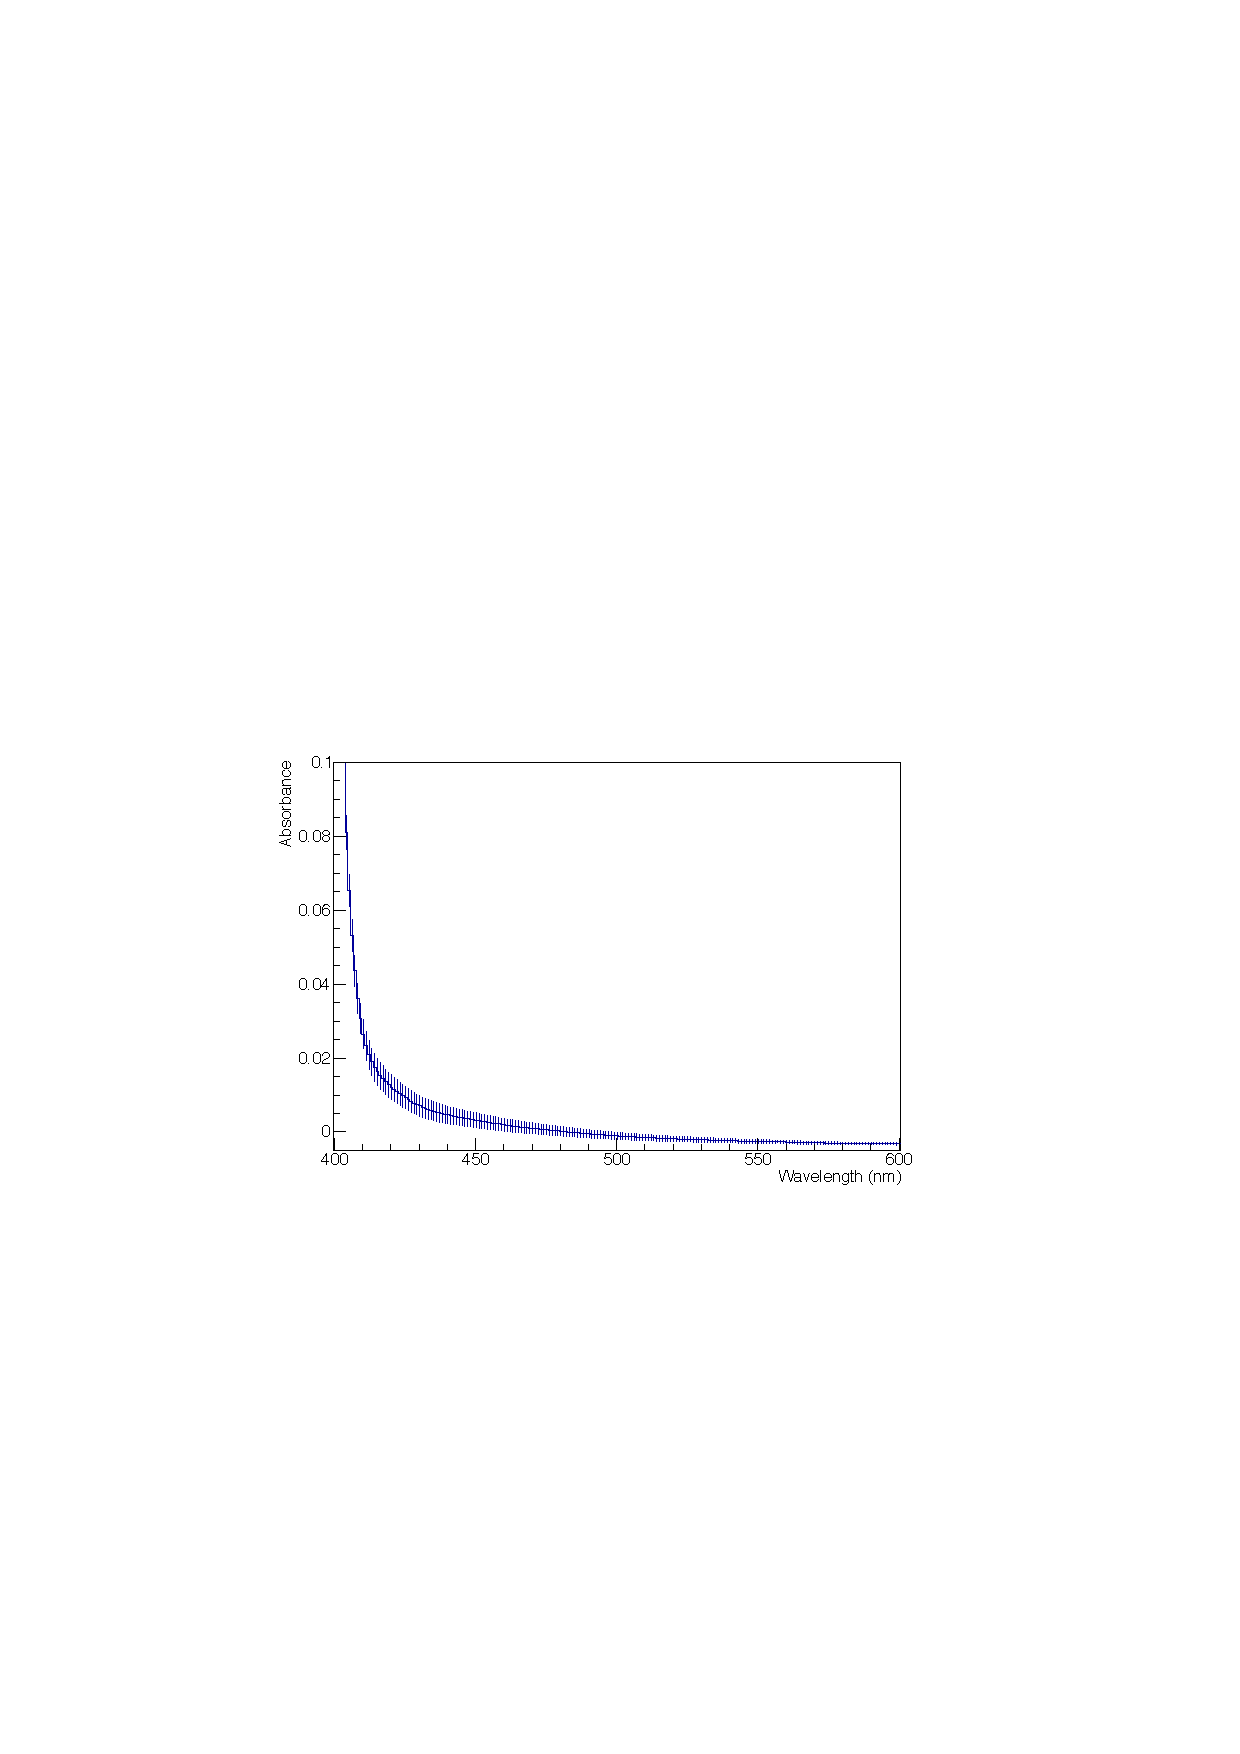
\includegraphics[width=0.5\textwidth]{Figures/LSQA1.pdf}\\
    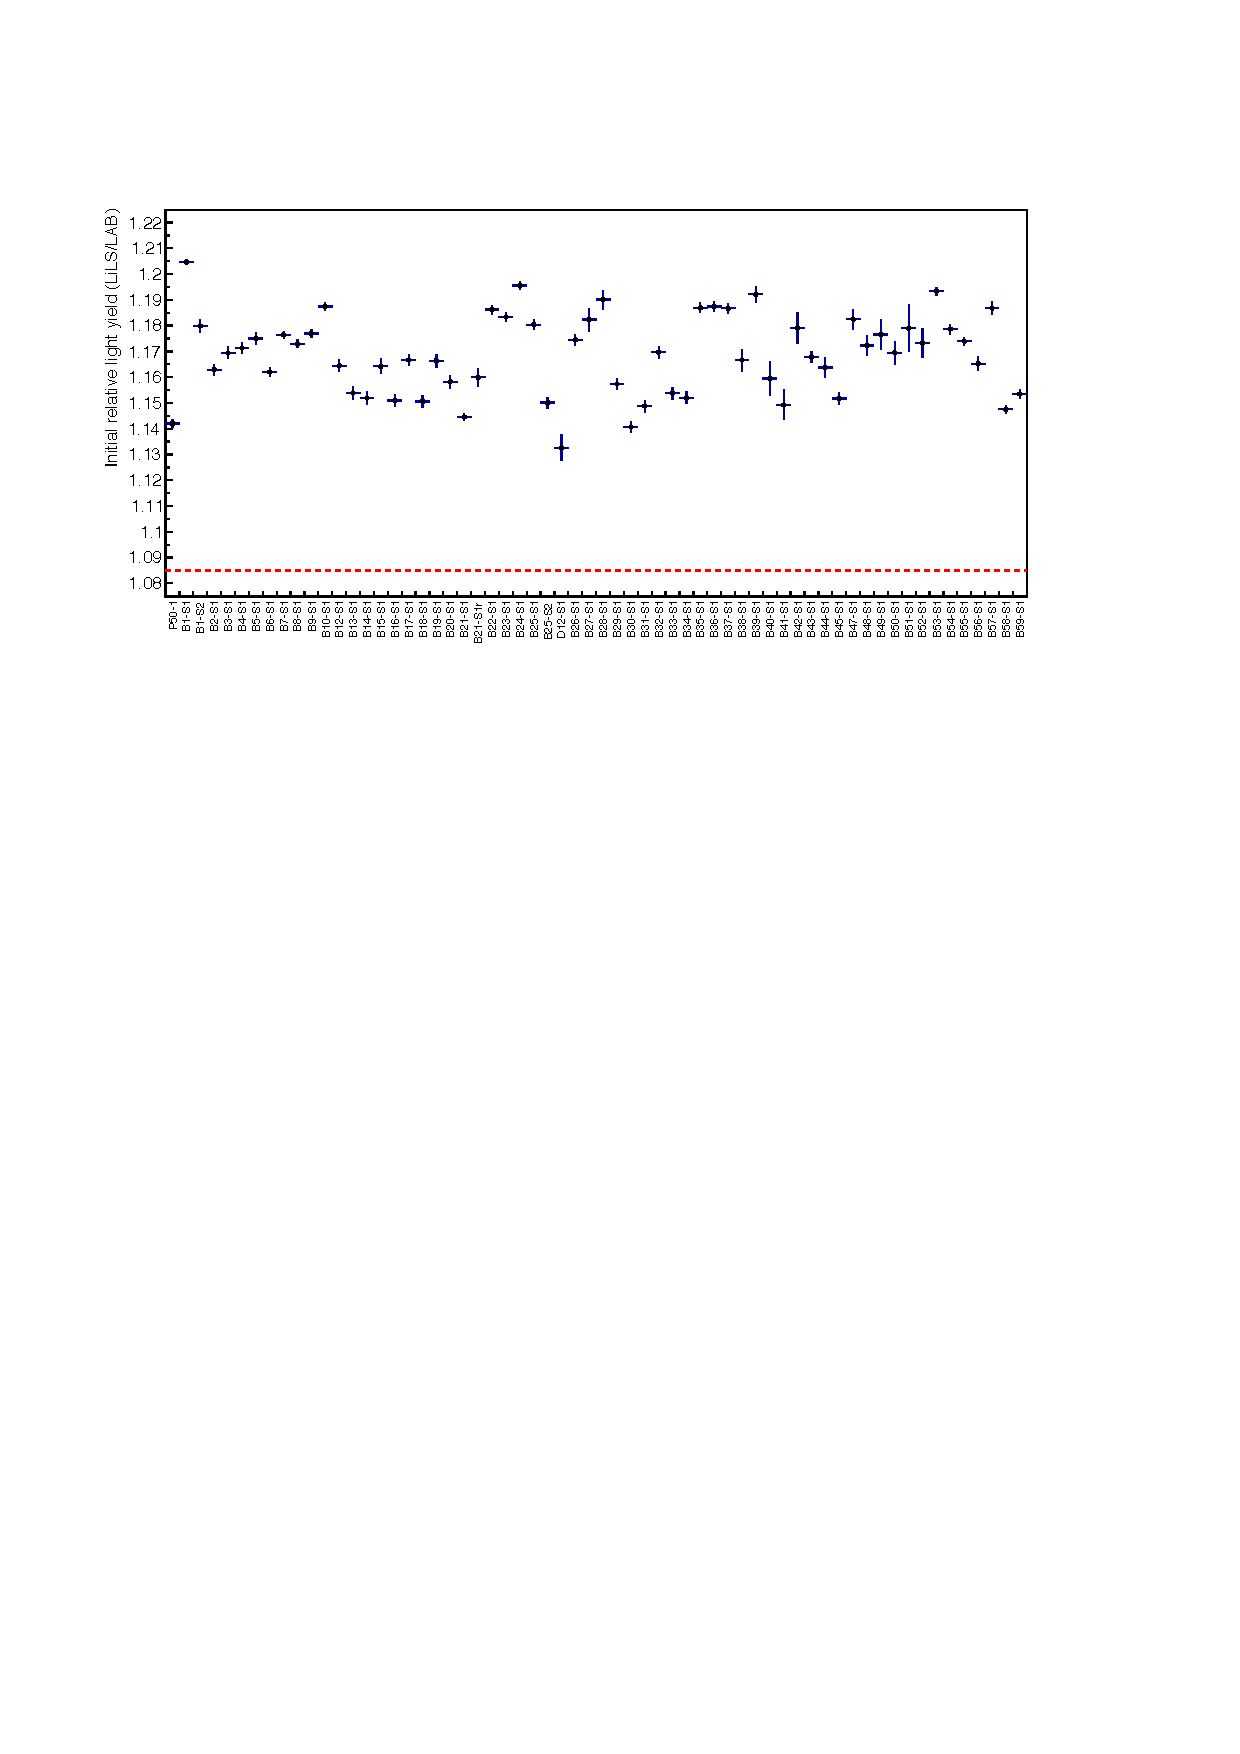
\includegraphics[width=0.9\textwidth]{Figures/LSQA2.pdf}\\
    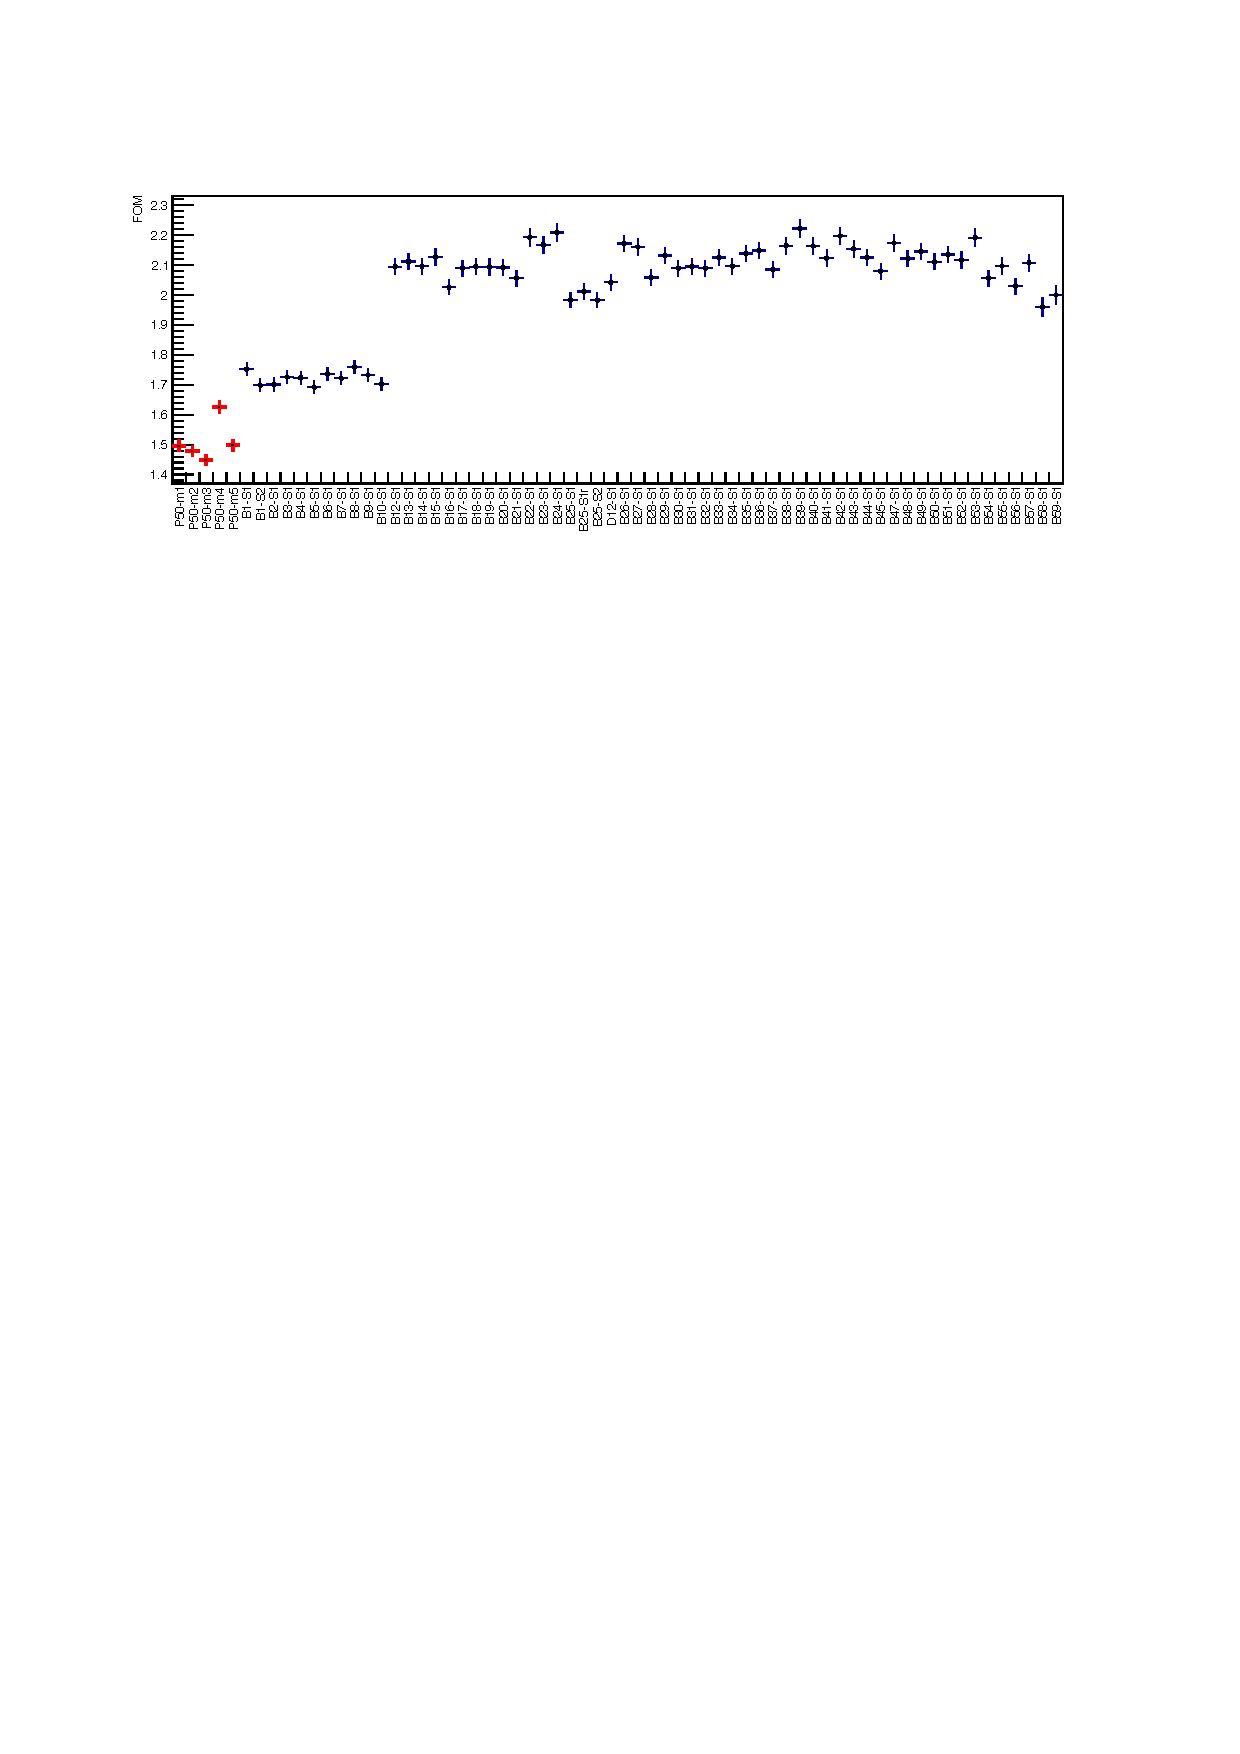
\includegraphics[width=0.9\textwidth]{Figures/LSQA3.pdf}\\
    \caption[The QA measurements of the $^6$LiLS]{(Top) The average of the relative absorbance of all the measured LiLS samples.
    (Center) The relative light yield ratio between $^6$LiLS and LAB.
    (Bottom) The FOM evaluated from each batch of product $^6$LiLS. \cite{bib:lspaper}}
    \label{fig:LSQA}
\end{figure}

\Section{Optical Grid}
\label{sec:OG}

The neutrino oscillation measurement in PROSPECT needs a position-sensitive IBD detector.
Because the available site for PROSPECT AD deployment has less than one~meter water equivalent (m.w.e) overburden, the PROSPECT AD should also be designed as a particle track sensitive detector to identify cosmogenic backgrounds.
The optical grid subsystem is thus a vital structure for both of PROSPECT's primary neutrino physics goals.
This subsystem is designed to meet the goals of:
\begin{itemize}
	\item Minimizing the inactive volume and mass;
	\item Maximizing the light collection efficiency with high reflectivity;
	\item Minimizing the cross-segment light transmission;
	\item Ensuring material compatibility with $^6$LiLS;
	\item Enabling the calibration system's installation in the detector volume.
\end{itemize}
The major components of the optical grid were designed and fabricated at IIT.
I played key roles in the material searching, fabrication, QC and QA tests, and construction of this subsystem.
An article was published by the IIT group of PROSPECT, see Reference \cite{bib:prospect_og}.

\Subsection{Optical Grid Design}
The structure of the optical grid is shown in Figure~\ref{fig:OGDesign}.
This subsystem consists of specular reflective separators and 3D printed polylactic acid (PLA) rods. 
The separators and PLA rods interlock each other to assemble a stable 14$\times$11 grid structure, whose dimensions can be found in Table~\ref{tab:PROSPECT_AD}.
The interlocking pieces enforce a $\sim5^\circ$ tilted angle for each segment.
The segments of the optical grid are enclosed by 154 PMT modules on each end, forming the inner detector structure which is supported by external acrylic supports.

\begin{figure}[h!]
\centering
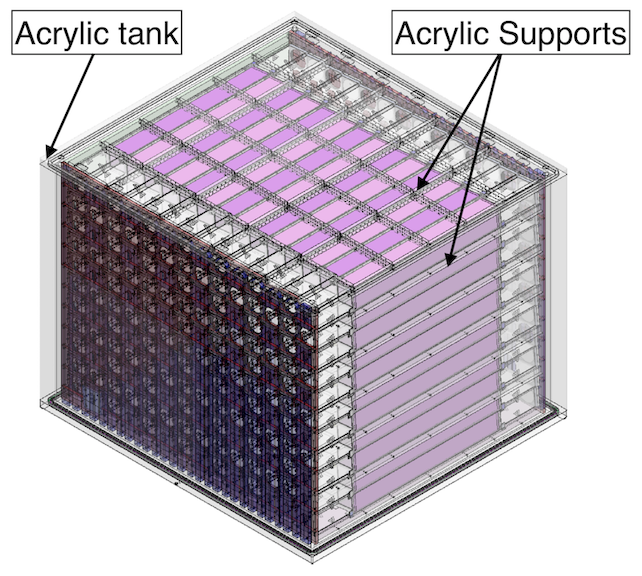
\includegraphics[clip, width=0.4\textwidth]{Figures/DetailedDetector.png} \\
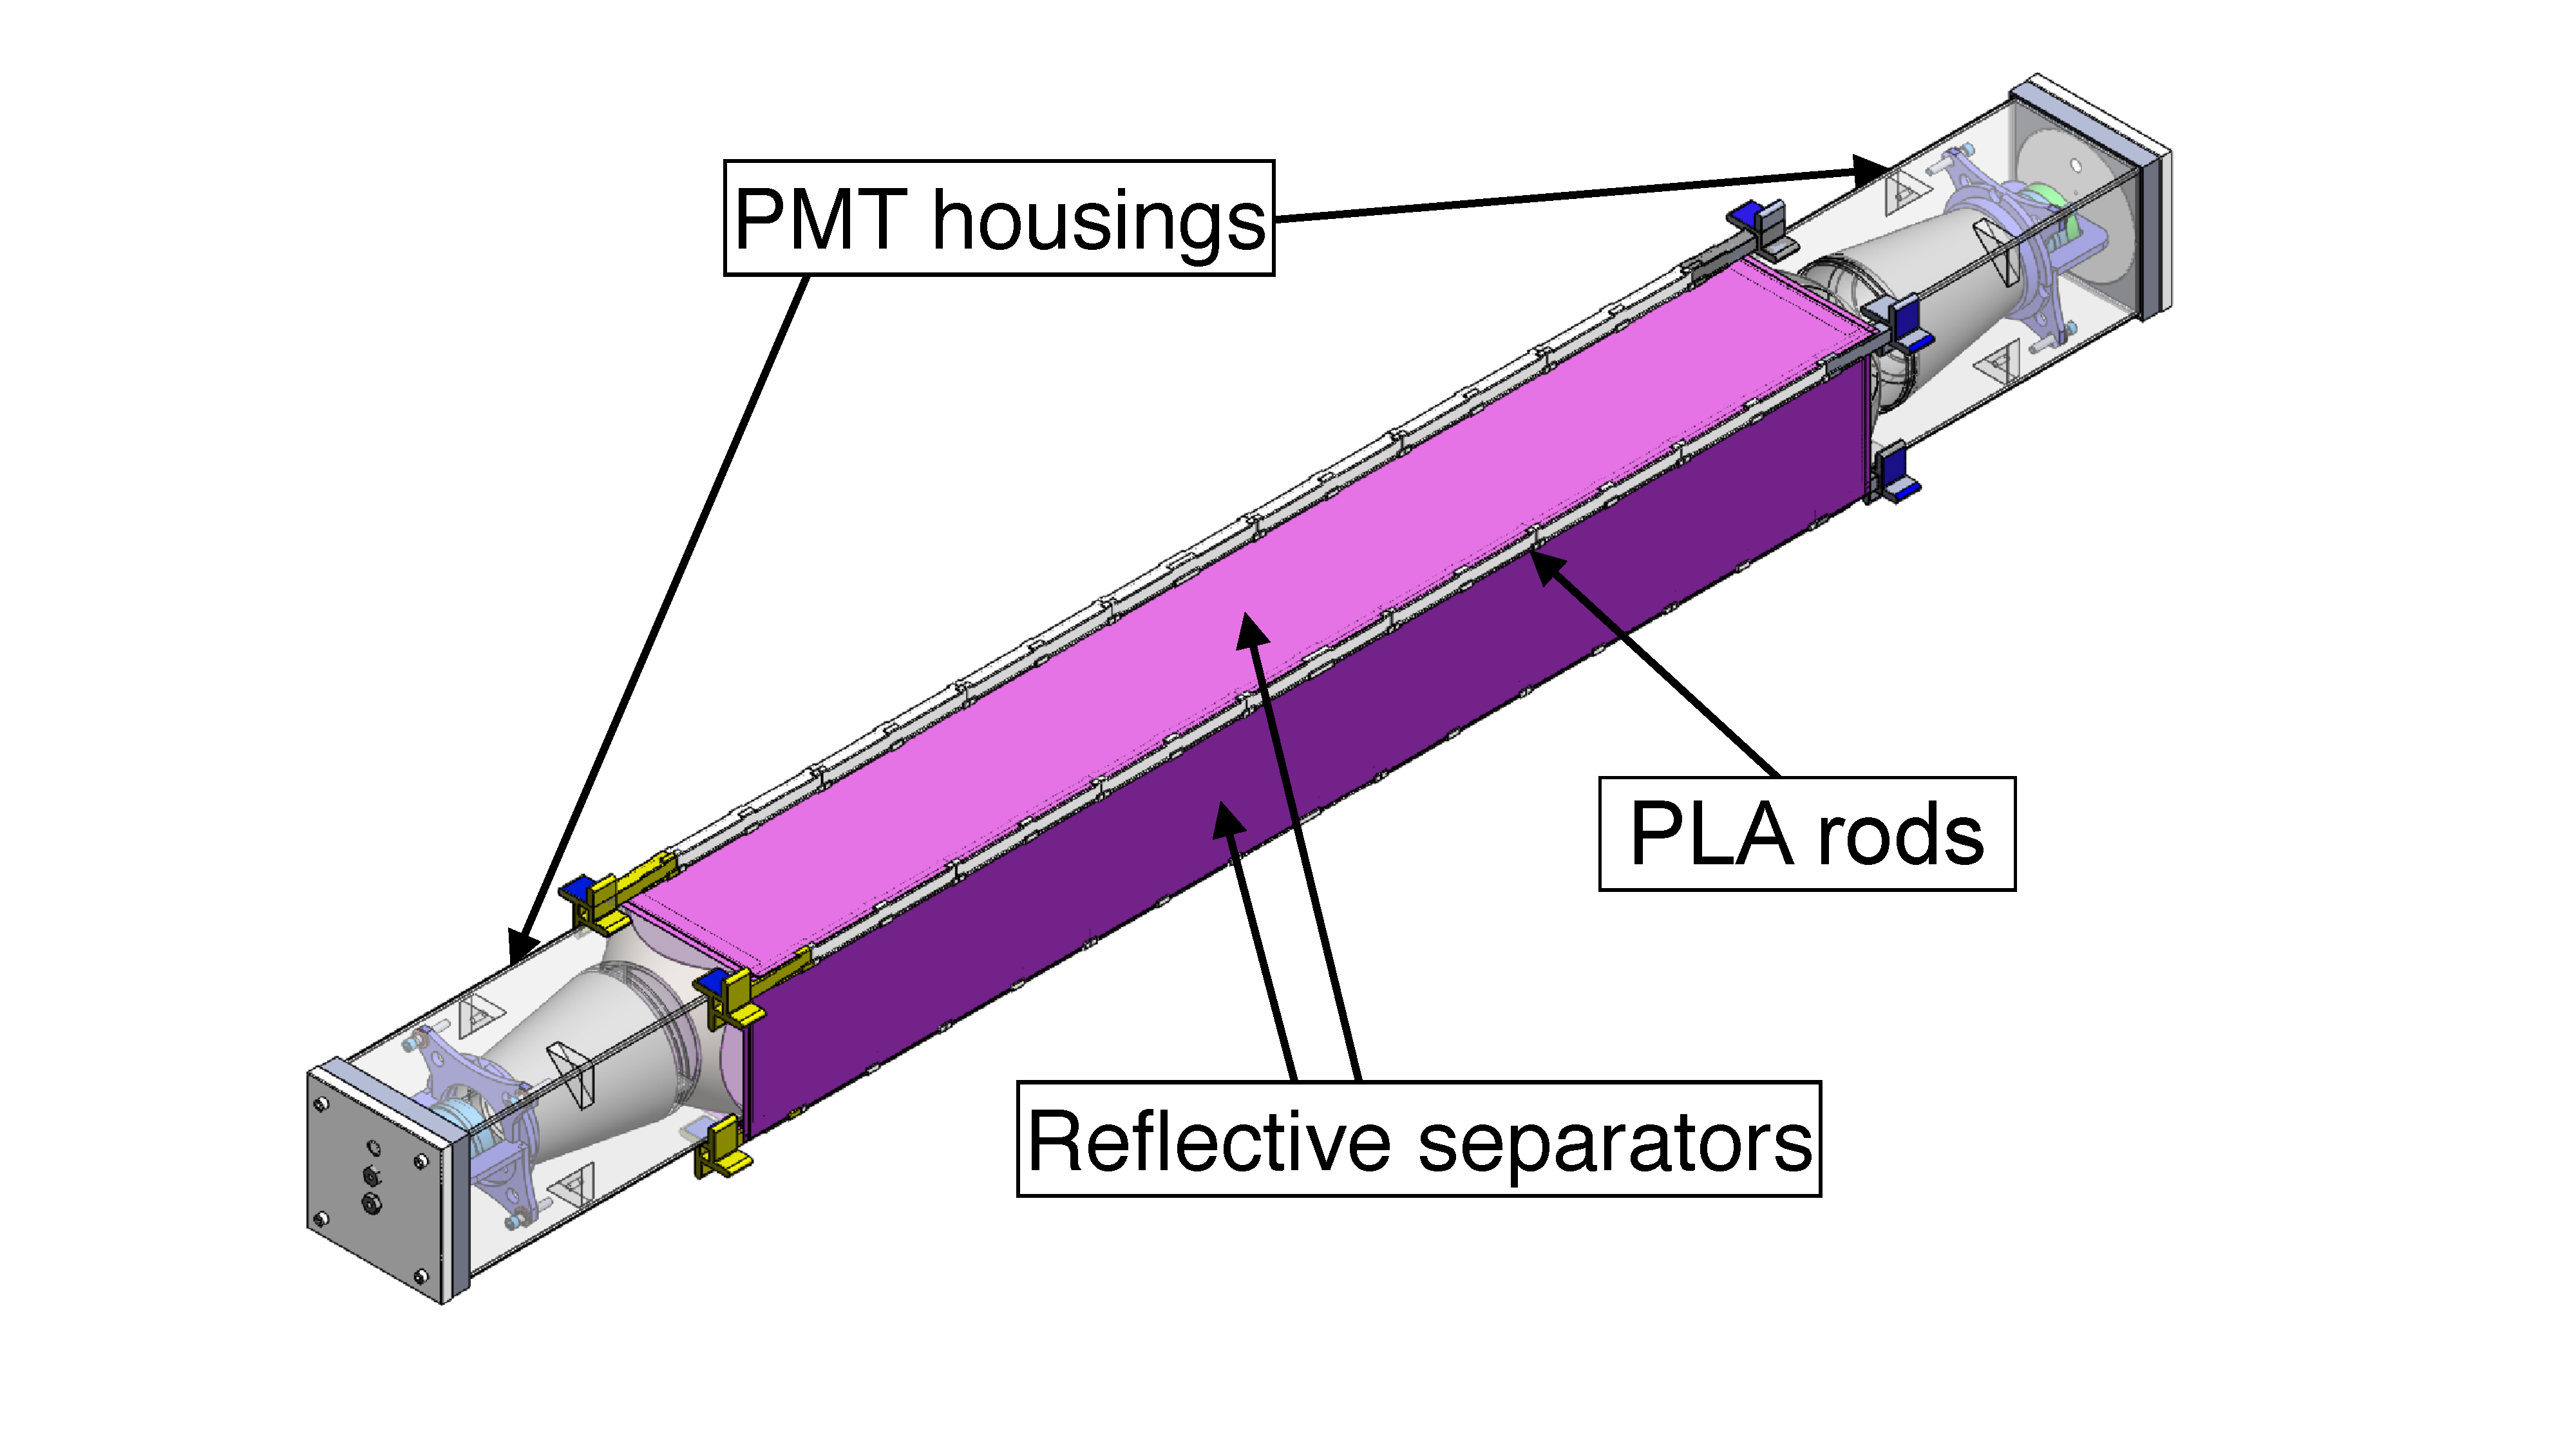
\includegraphics[trim = 2cm 2cm 2cm 2cm,clip, width=0.47\textwidth]{Figures/DetailedSegment.pdf} 
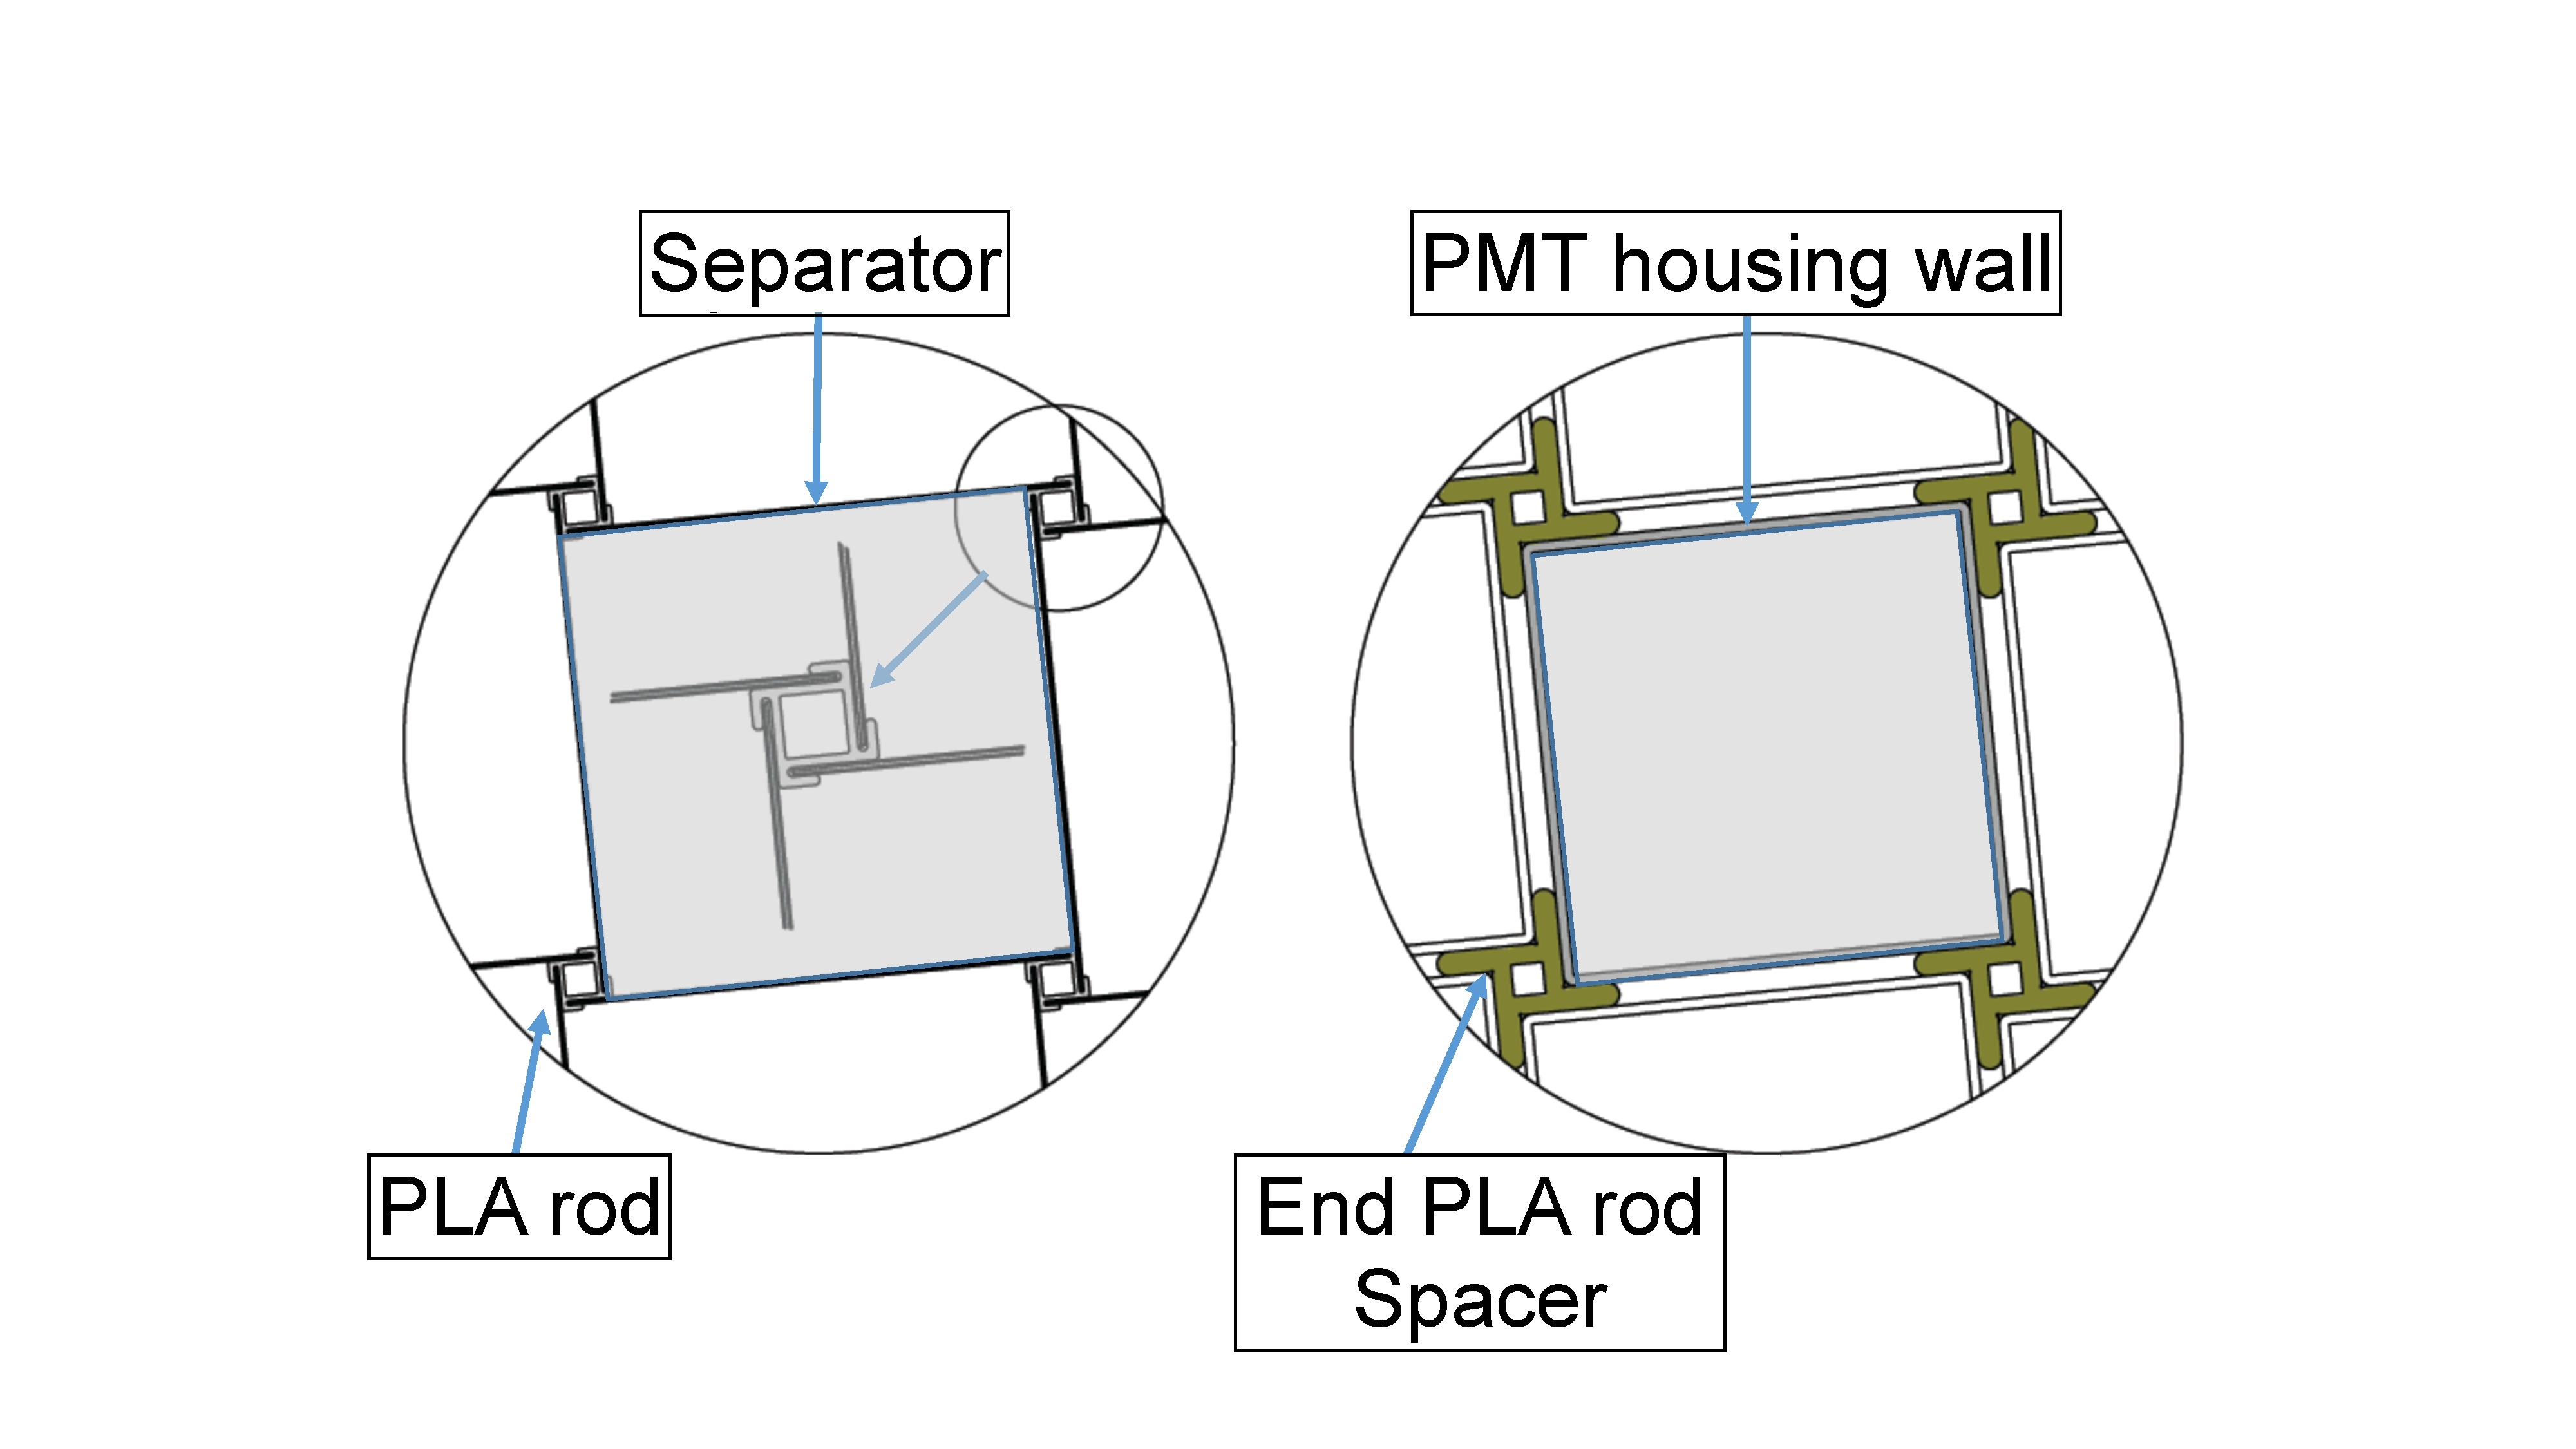
\includegraphics[trim = 2cm 2cm 2cm 2cm,clip, width=0.52\textwidth]{Figures/DetailedOGDesign.pdf}
\caption[Detailed PROSPECT optical grid schematic] {Detailed PROSPECT optical grid schematic. 
(Top) The active detector enclosed by liquid-tight sealed acrylic tank. 
(Bottom left) The individual segment with a 12.7~cm (5~in) diameter PMT on each end and enclosed by 4 reflective separators. 
(Bottom right) The cross section view of the PLA rods and segment, where the separators are slotted on the PLA rods and the PLA rods are hollow to allow calibration sources to be inserted.}
\label{fig:OGDesign}
\end{figure} 

\Subsection{Separators}
The separators are composed of a laminated sandwich of a carbon fiber backbone, reflector layers, adhesive layers, and 0.05~mm-thick protective Fluorinated Ethylene Propylene (FEP)  films, as shown in Figure~\ref{fig:panel_scheme}.
Except for the FEP film, poor compatibility between the separator materials and the $^6$LiLS was found in chemical compatibility tests.
In order to prevent direct contact between the $^6$LiLS and the incompatible materials, the FEP protective films were heat-sealed and folded, as illustrated in Figure~\ref{fig:panel_scheme} (right).
	
\begin{figure}[h!]
\centering
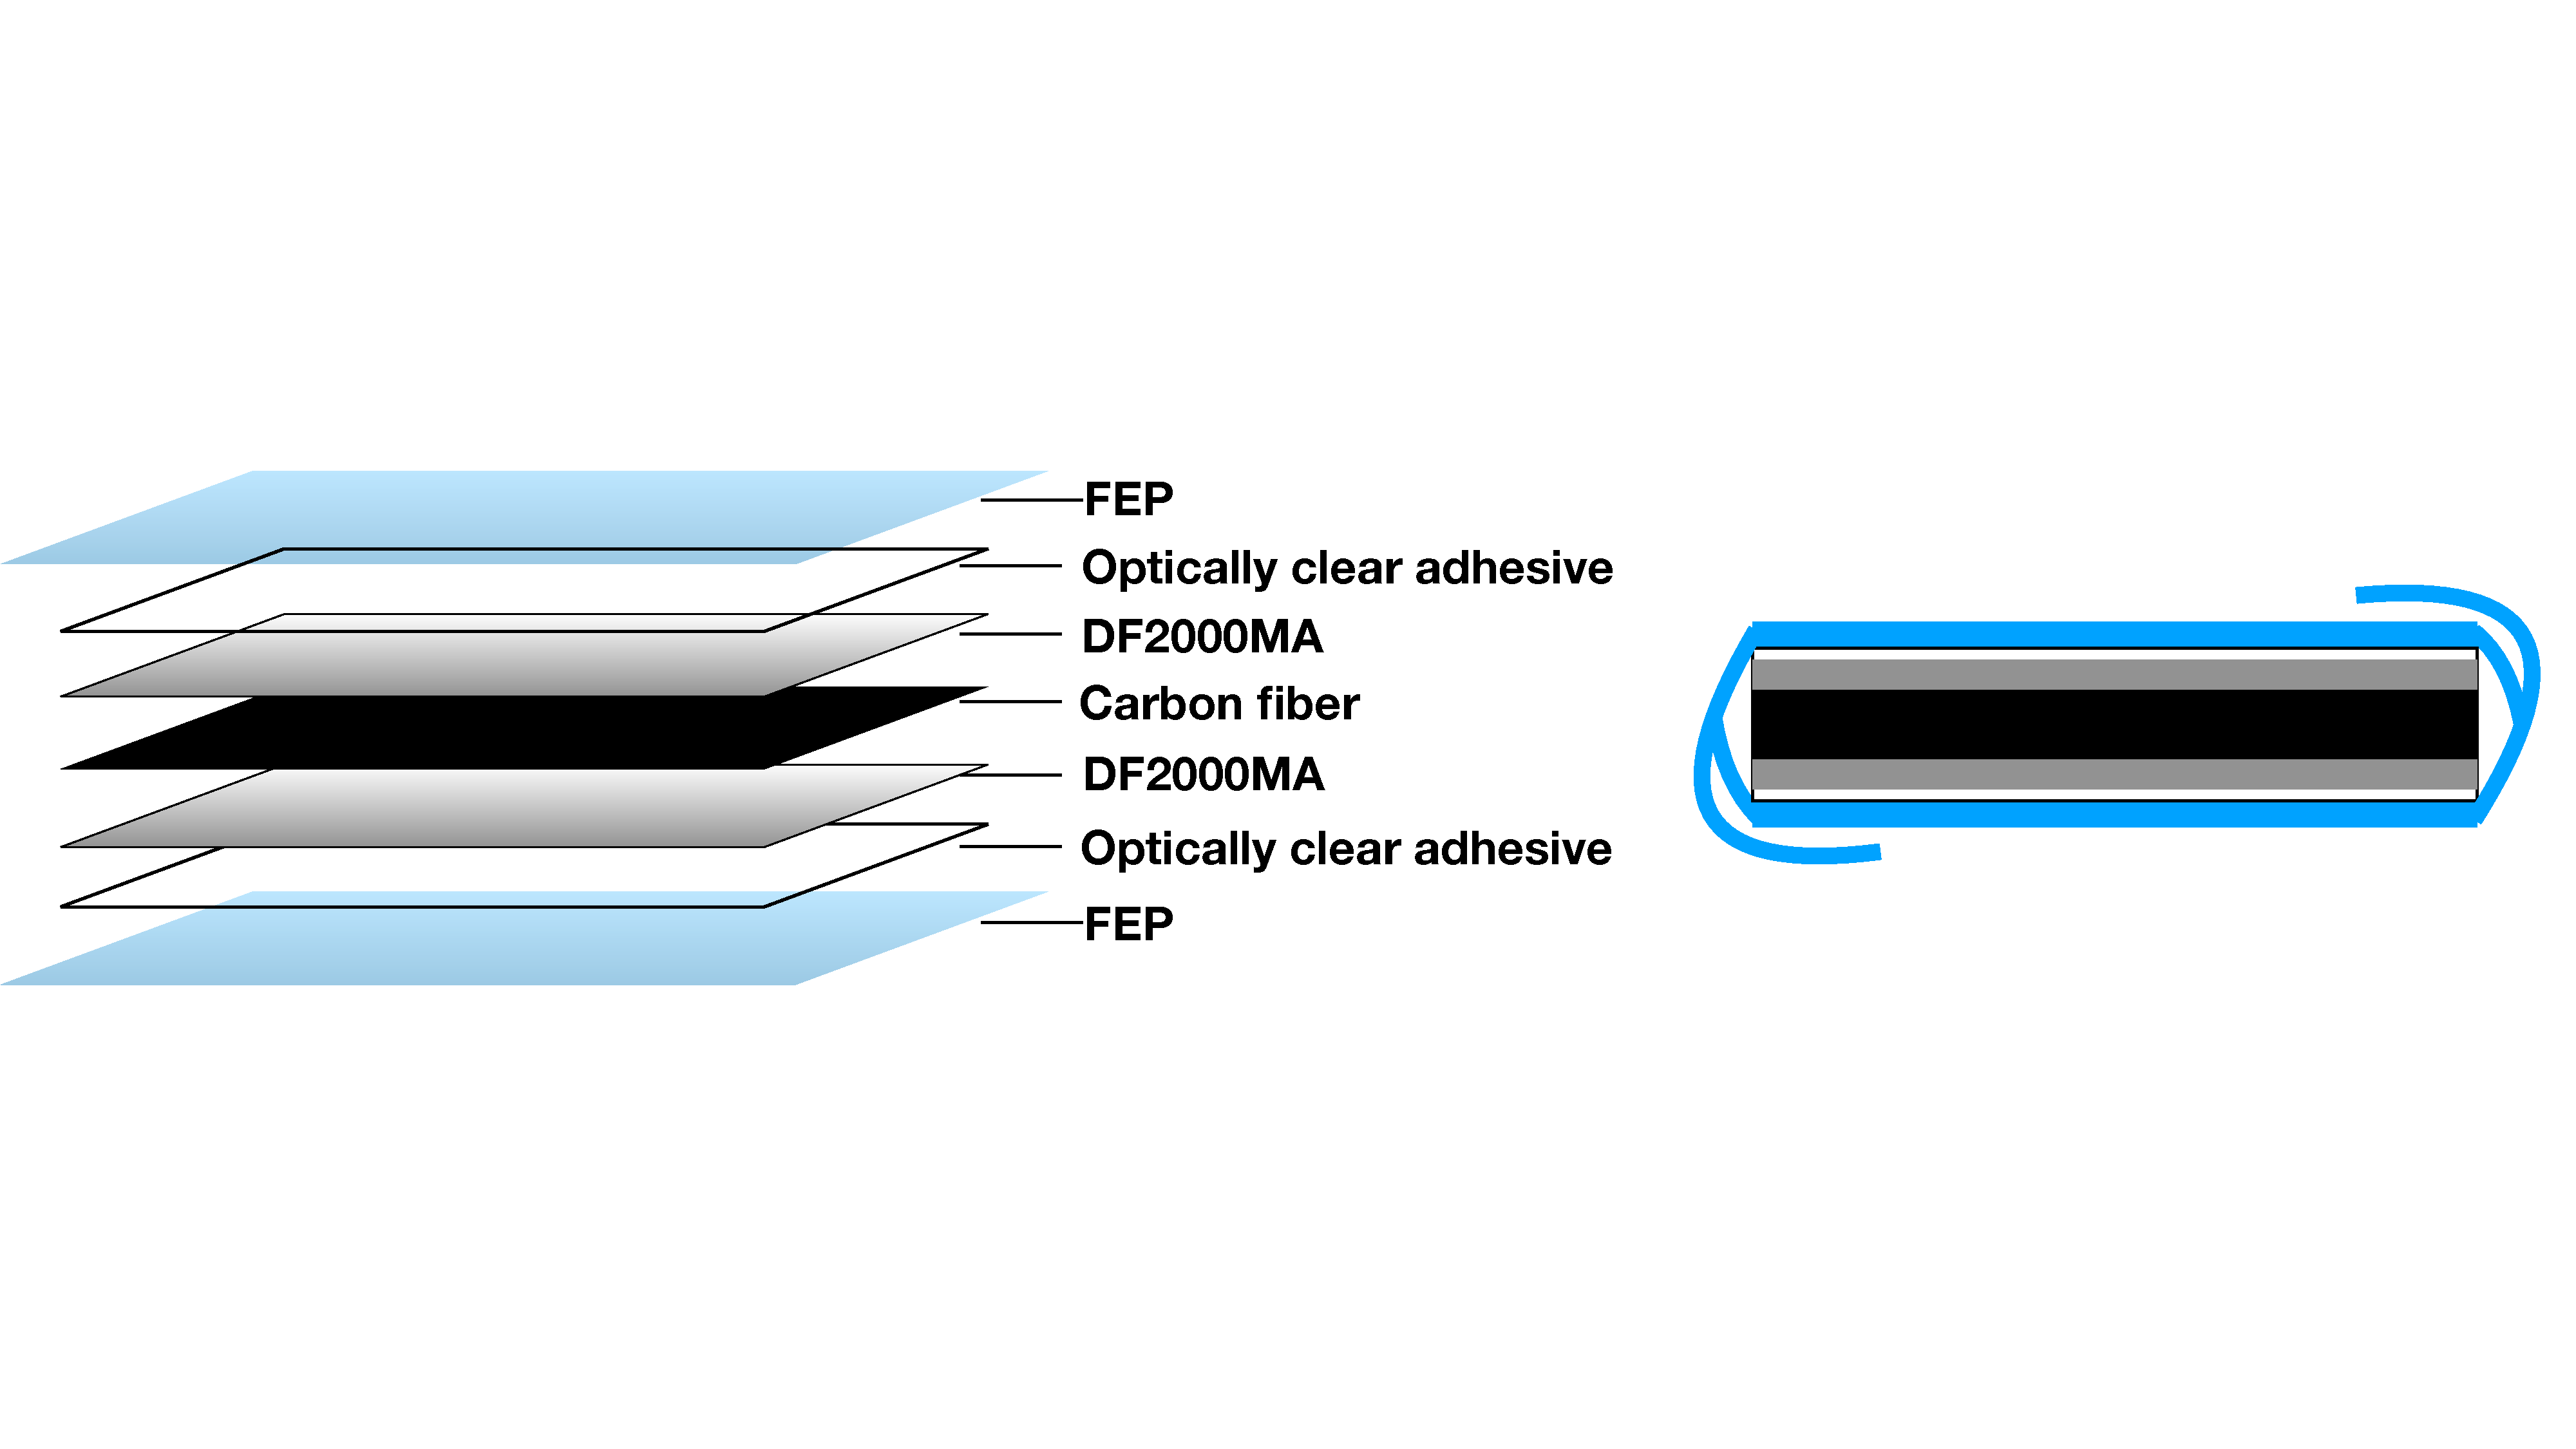
\includegraphics[trim = 0.0cm 8.0cm 0.0cm 10.0cm, clip=true, width=0.9\textwidth]{Figures/panel_schematic2.pdf} 
%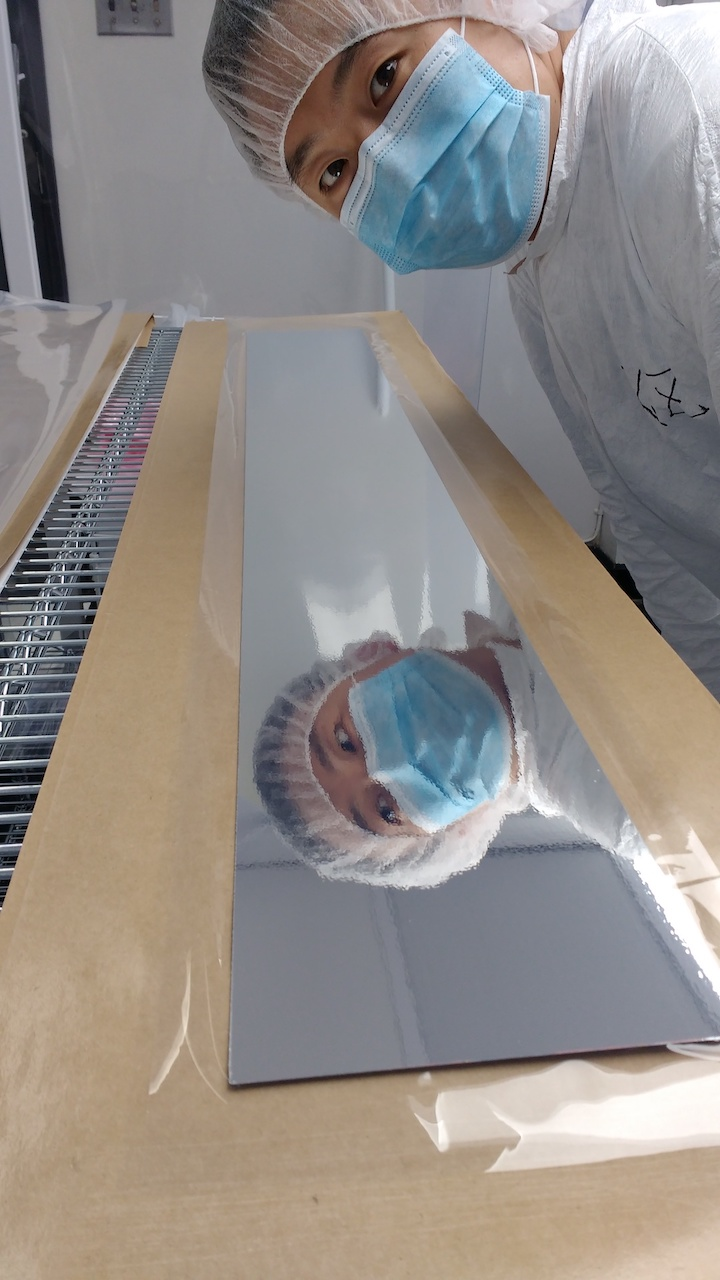
\includegraphics[trim = 0.0cm 13.0cm 0.0cm 27.0cm, clip=true, width=0.35\textwidth]{figures/Separator.jpg}
%\includegraphics[clip=true, width=0.6\textwidth]{figures/WrappedPanel.JPG}
\caption[Illustration of a separators sandwich structure]{(Left) Illustration of the sandwich structure of a separator. 
(Right) Illustration of the separator with the overhung FEP folded. }
\label{fig:panel_scheme}
\end{figure}

Table~\ref{tab:separator_dimension} lists designed and measured optical grid component dimensions.
The total length of the separators, excluding the heat-sealed overhanging FEP, was designed to be 120.65~cm $\pm$ 0.25~cm (47.5~in $\pm$ 0.1~in).  
The designed distance between the front surfaces of the two PMT housings is 117.4~cm (46.25~in), with the reflecting separator surface extending beyond the front windows of the PMT housings and out of the active optical volume of the segment.  
Since the separators extend past the faces of the PMT housings, the tolerances on the separator length are not stringent.  
Based on the PMT housing dimensions and extra width needed for securely coupling to the PLA rods, the nominal width of separators was designed to be 15.35~cm $\pm$ 0.04~cm.
The summed thickness of all laminated material is 1.03~mm $\pm$ 0.1~mm.
Accounting for the allowed thickness of the assembly with the PLA rods and the imperfect coupling between each two-layers, the allowed and measured thickness is higher than the summed thickness of all individual layers.

\begin{table}[htpb]
\centering
\caption{Designed and measured dimensional parameters of separators.}
\begin{tabular}{cc}
\hline
\hline 
Material & Dimensions and tolerance (mm) \\ \hline 
Nominal length & 1206.5 $\pm$ 2.5 \\
Nominal width & 153.5 $\pm$ 0.4 \\
Nominal thickness (sum of material thickness)  & 1.03 $\pm$ 0.1 \\ 
Allowed thickness for assembly  & 1.119-1.124 \\ \hline
Measured width & 153.6 $\pm $0.6 \\
Measured thickness & 1.18 $\pm$ 0.05 \\
\hline
\end{tabular}
\label{tab:separator_dimension}
\end{table}

The reflective material used is DF2000MA, an adhesive-backed organic reflecting film.
DF2000MA is made of multiple polymer layers with varying refractive indices, which produce multiple total internal reflections~\cite{bib:ESR_science}.
Among the tested materials in PROSPECT R\&D, DF2000MA exhibits superior specular reflectance in the range of wavelength from 400~nm to 550~nm, as shown in Figure~\ref{fig:refcomp}.
The FEP film was laminated on top of the DF2000MA with optically clear adhesives.
Having a substantially lower index of refraction than the $^{6}$LiLS ($\sim$1.3 versus $\sim$1.55, respectively), the FEP film also ensures total internal reflection of grazing angle incident scintillation light back into the $^{6}$LiLS bulk.  

\begin{figure}[h!]
\centering
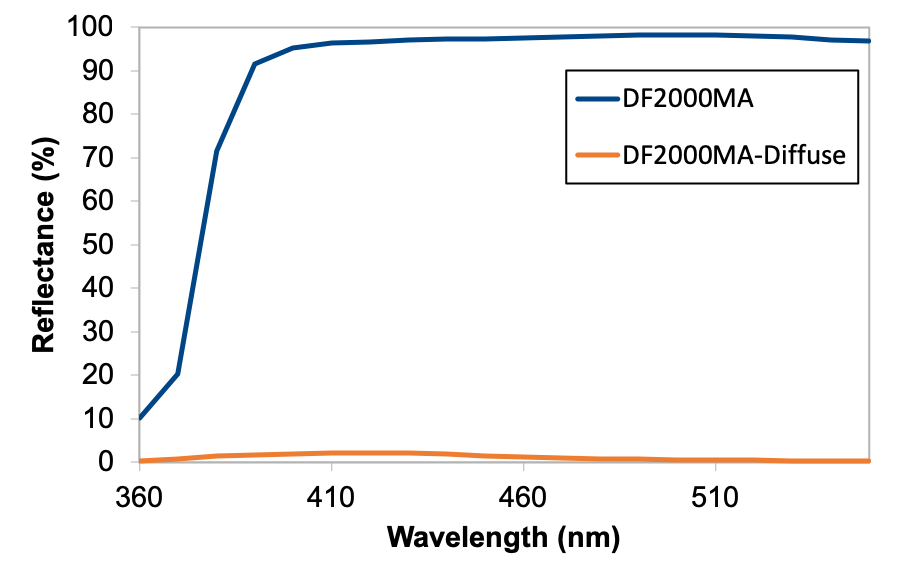
\includegraphics[trim = 0mm 0cm 0cm 0cm, clip, width=0.49\textwidth]{Figures/ReflectorCompare.png}
\caption[Reflectance measurement of DF2000MA]{Total reflectance and diffuse reflectance of DF2000MA.}
\label{fig:refcomp}
\end{figure}

The lamination of all separators was conducted in a class 10000 clean tent at IIT.
Each layer of different material was laminated at room temperature with a silicon roll laminator.
Because the puncture of FEP film can cause exposure of inner separator materials to the $^6$LiLS, the lamination procedures were designed to minimize the possibility of causing scratches on separator surfaces or leaving dust between layers.
Photographs of the lamination process and a laminated separator are shown in Figure~\ref{fig:laminationPic}.
In the end, each separator was labeled with stickers on the excess of FEP film for QC and QA purposes, then shipped to a company specializing in heat sealing FEP films.

\begin{figure}[h!]
\centering
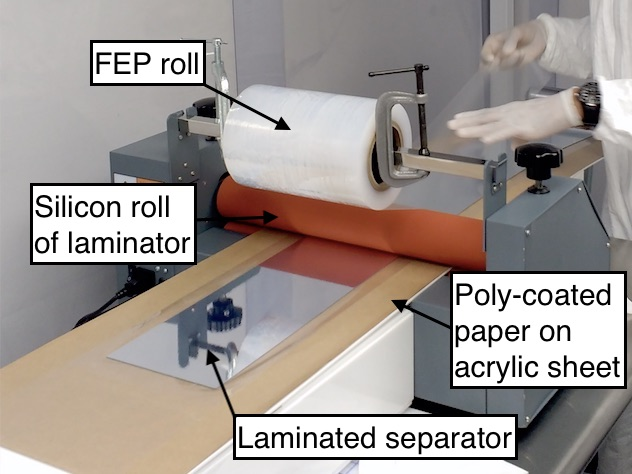
\includegraphics[width=0.5\textwidth]{Figures/Lamination.jpg} \\
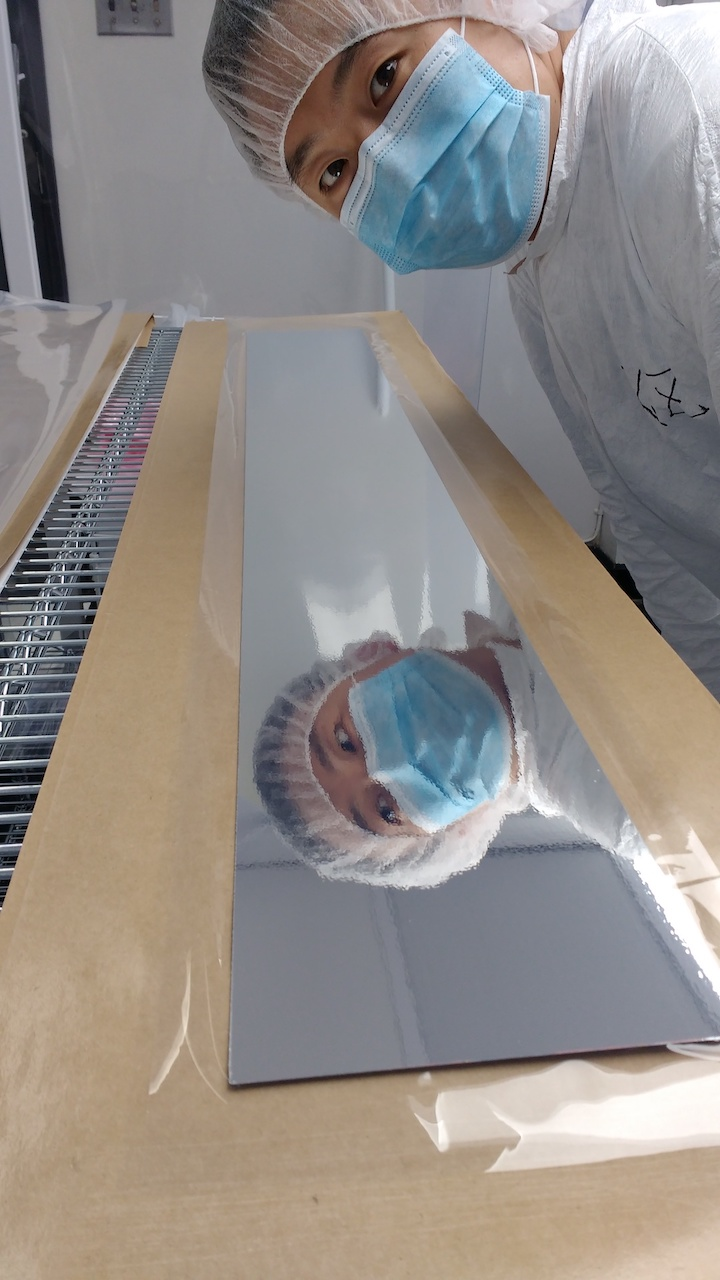
\includegraphics[trim = 0.0cm 2.0cm 0.0cm 8.0cm, clip=true, width=0.4\textwidth]{figures/Separator.jpg}
\caption[Separator lamination]{(Top) Photograph of lamination setup, when FEP film were being laminated on one side of separator.
(Bottom) Photograph of a laminated separator.}
\label{fig:laminationPic}
\end{figure}

The QA measurements of the separators includes surface quality evaluation, dimension measurements, reflectance measurements, and sealing tests.
Separators with wrinkles or dust whose diameter is greater than 1~mm were rejected.
A separator with width or thickness out of tolerance were also rejected. 
The total reflectance and diffuse reflectance of the separators was measured with a compact spectrometer in the fabrication cleanroom.
By measuring relative total reflectance compared to a small size separator sample, separators with visible optical defects were rejected.
Sealing tests were conducted twice, first after FEP heat sealing and then during final cleaning.
It was found during R\&D that the adhesive turns white in air when it is contacted with ethyl alcohol. 
Therefore, ethyl alcohol was applied on the separator surface to identify a puncture or failed sealing.
Separators passing the sealing tests were accepted for detector assembly.
The count of laminated separators that passed each level of QC is shown in Table~\ref{tab:separatorQA}.

\begin{table}[h!]
\centering
\caption[The count of fabricated separators passing each level of QC]{The count of laminated separators that passed each level of QC. 
98.6\% (367 out of 372) of laminated separators passed QC; 333 separators were assembled into the PROSPECT AD.}
\begin{tabular}{cc}
\hline 
\hline
QC level & Count of separators\\
\hline
Laminated & 372 \\
Surface quality & 371 \\
Optical QA & 370 \\
Dimensional QA & 369 \\
Heat sealing quality & 367 \\
Used in detector assembly & 333\\
\hline
\end{tabular}
\label{tab:separatorQA}
\end{table}

\Subsection{3D Printed PLA Rod}

The PLA rods were designed to support the separators with low density and low volume material, while contributing a precise interface between separators and other detector supporting structures.
In addition, the PLA rods provide enough free space for optical and radioactive calibration structures to feed through into the detector inner volume.
Fused Deposition Modeling (FDM) 3D printing was deemed to be the best choice for the production of the PLA rods.  This method of 3D printing has advantages of its ability to produce complicated geometries, a wide choice of materials, ease of prototyping, and minimal setup cost.
Among the tested materials for 3D printing, PLA was found compatible to $^6$LiLS.
Using white-dyed PLA, PROSPECT also takes advantage of its high diffuse reflectivity and low light transmission, as shown in Figure~\ref{fig:PinwheelOptic}.

\begin{figure}[h]
\centering
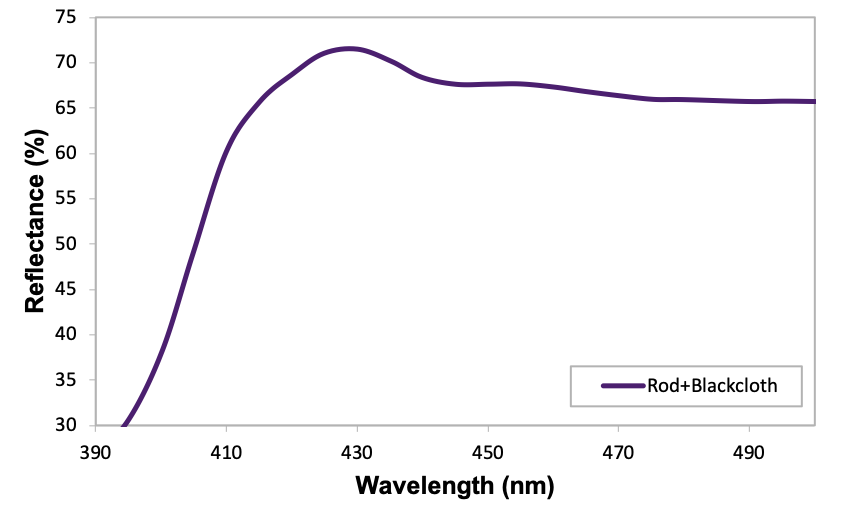
\includegraphics[width=0.48\textwidth]{Figures/PinwheelDiff.png} \quad
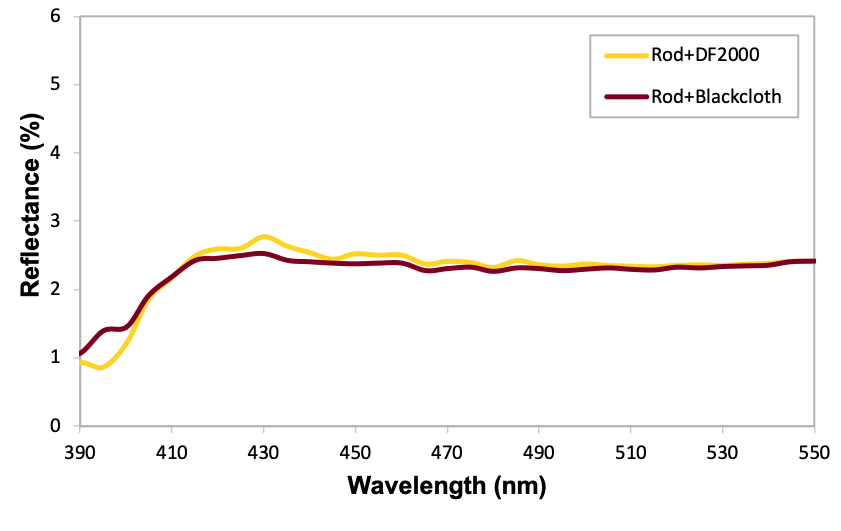
\includegraphics[width=0.48\textwidth]{Figures/PinwheelSpec.png}
\caption[Optical measurement on the PLA rods]{(Left)~Absolute diffuse reflectance of PLA
  rods. 
(Right)~Total reflectance of PLA rods relative to bare
  DF2000MA. 
When PLA was backed by DF2000MA reflector, the reflectance can be compared against the measurement of PLA backed by a black cloth to indicate the transmission of light. }
\label{fig:PinwheelOptic}
\end{figure}

The PLA rods are longitudinal tubes with a square cross-section.
There are small tabs printed on the outer surface for interlocking with the separators, forming a pinwheel-shaped cross-section.
Because of the part failure rate and the limited size of available 3D printers, all PLA rods are no more than 15.69~cm in length.
There are nine types of PLA rods designed according to their location in the assembled detector, as shown in Figure \ref{fig:pinwheel_types}. 
These nine types can be categorized into three main categories listed below.
\begin{itemize}
	\item Standard PLA rods: A 15.69~cm long rod with the tabs at its center and each end to allow the insertion of separators. 
The tabs on the ends are $\sim$6~mm long, and the tab at the center is $\sim$13~mm long to balance the structural stability and reflector exposure.
Among the standard PLA rods, there are PLA rods slightly longer to accurately fit the length of each segment and ensure light-tight closure between segments.
These standard PLA rods are labeled as type-1 and type-9, respectively.
There are 720 (360) type-1 (type-9) PLA rods needed in the PROSPECT AD.
	\item Center PLA rods: Similar to the standard PLA rod but with a 2.54~cm (1~in) wide center tab that allows further machining for the insertion of optical calibration system components.
The center PLA rods are labeled as type-2.
There are 180 type-2 PLA rods needed in the PROSPECT AD.
	\item End PLA rods: A 9.53~cm long rod whose one end is a standard tab for the separator to insert and whose other end is a pinwheel-shaped, thick, rigid spacer to maintain set spacings between PMT modules and strung PLA rods. The number of arms on the spacers depends on the location of rods in the detector.
The end PLA rods are labeled as type-3 to type-8.
There are 360 end PLA rods needed in the PROSPECT AD.
\end{itemize}

\begin{figure}[h!]
\centering
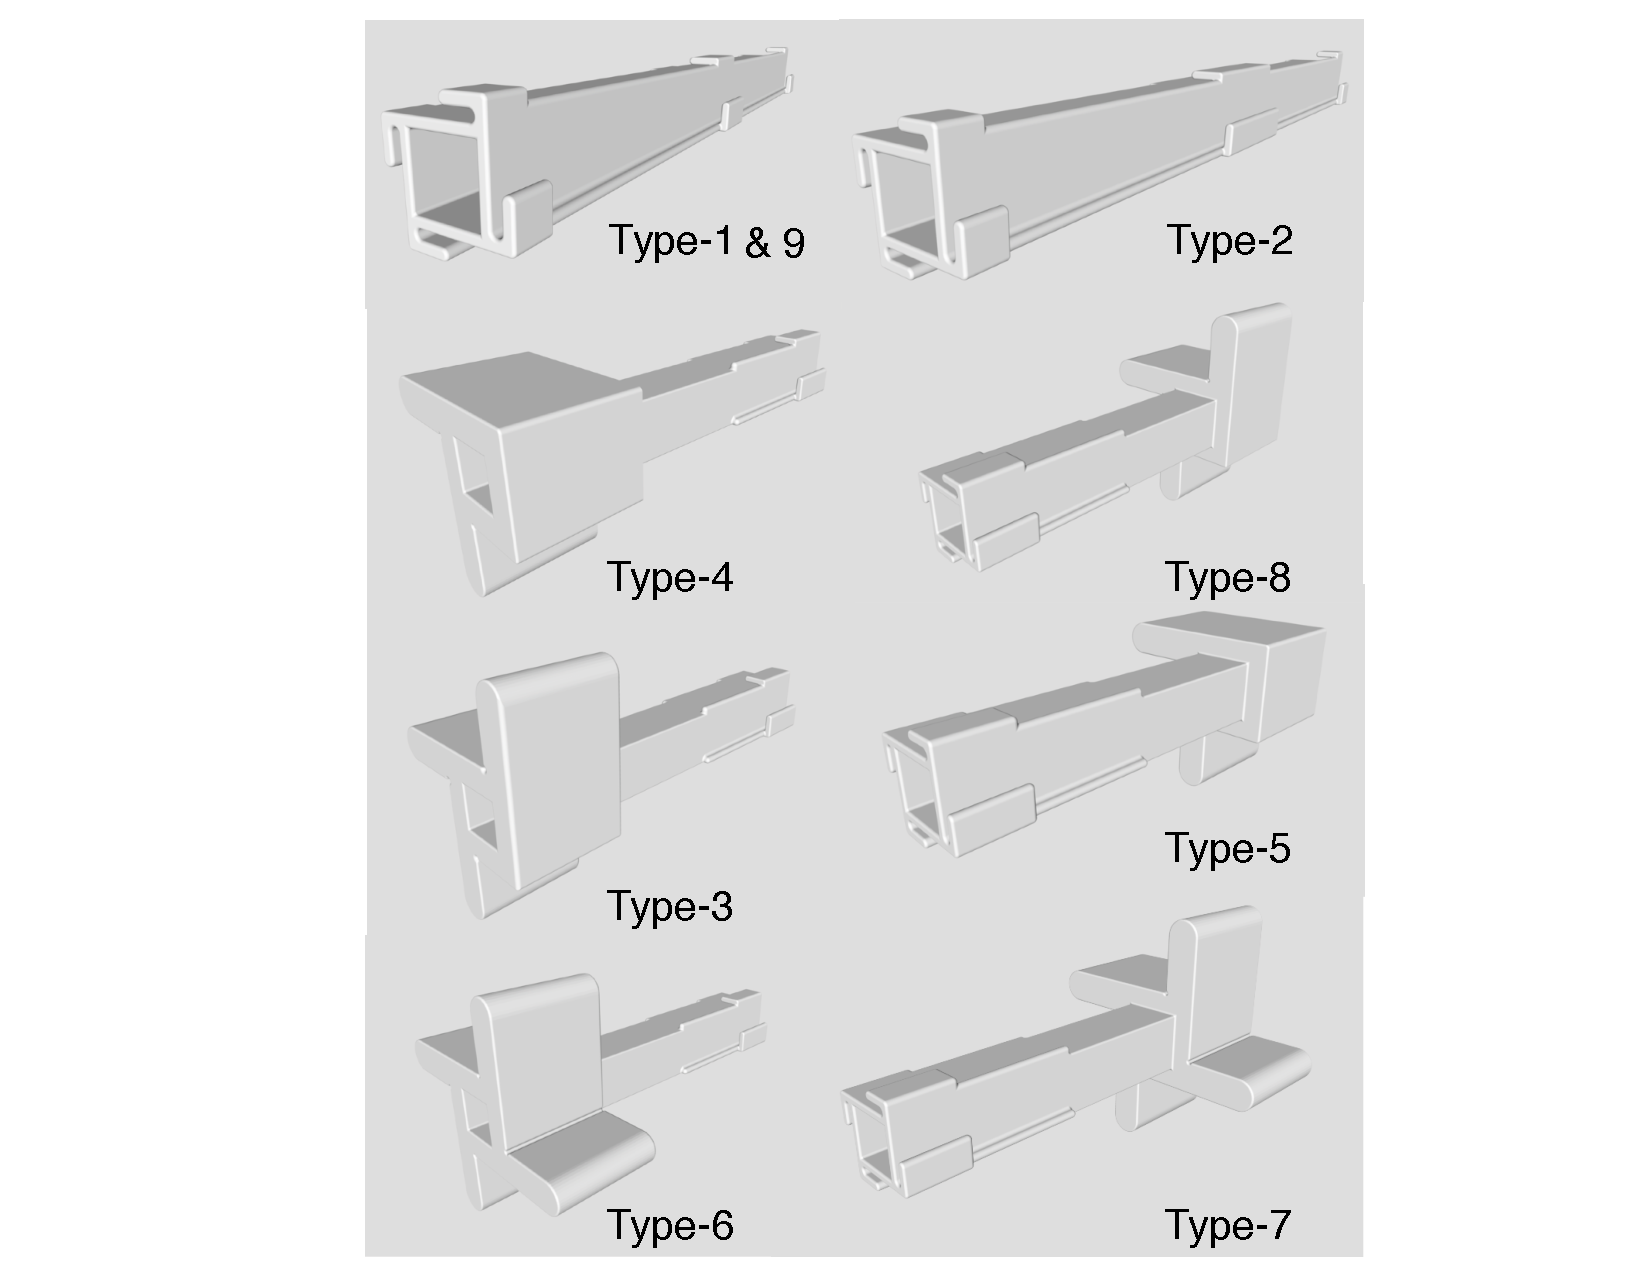
\includegraphics[width=0.8\textwidth]{Figures/Pinwheel_Types.pdf}
\caption[Schematics of PLA rods]{Schematic of PLA rods labeled by type.}
\label{fig:pinwheel_types}
\end{figure}

\begin{figure}[h!]
\centering
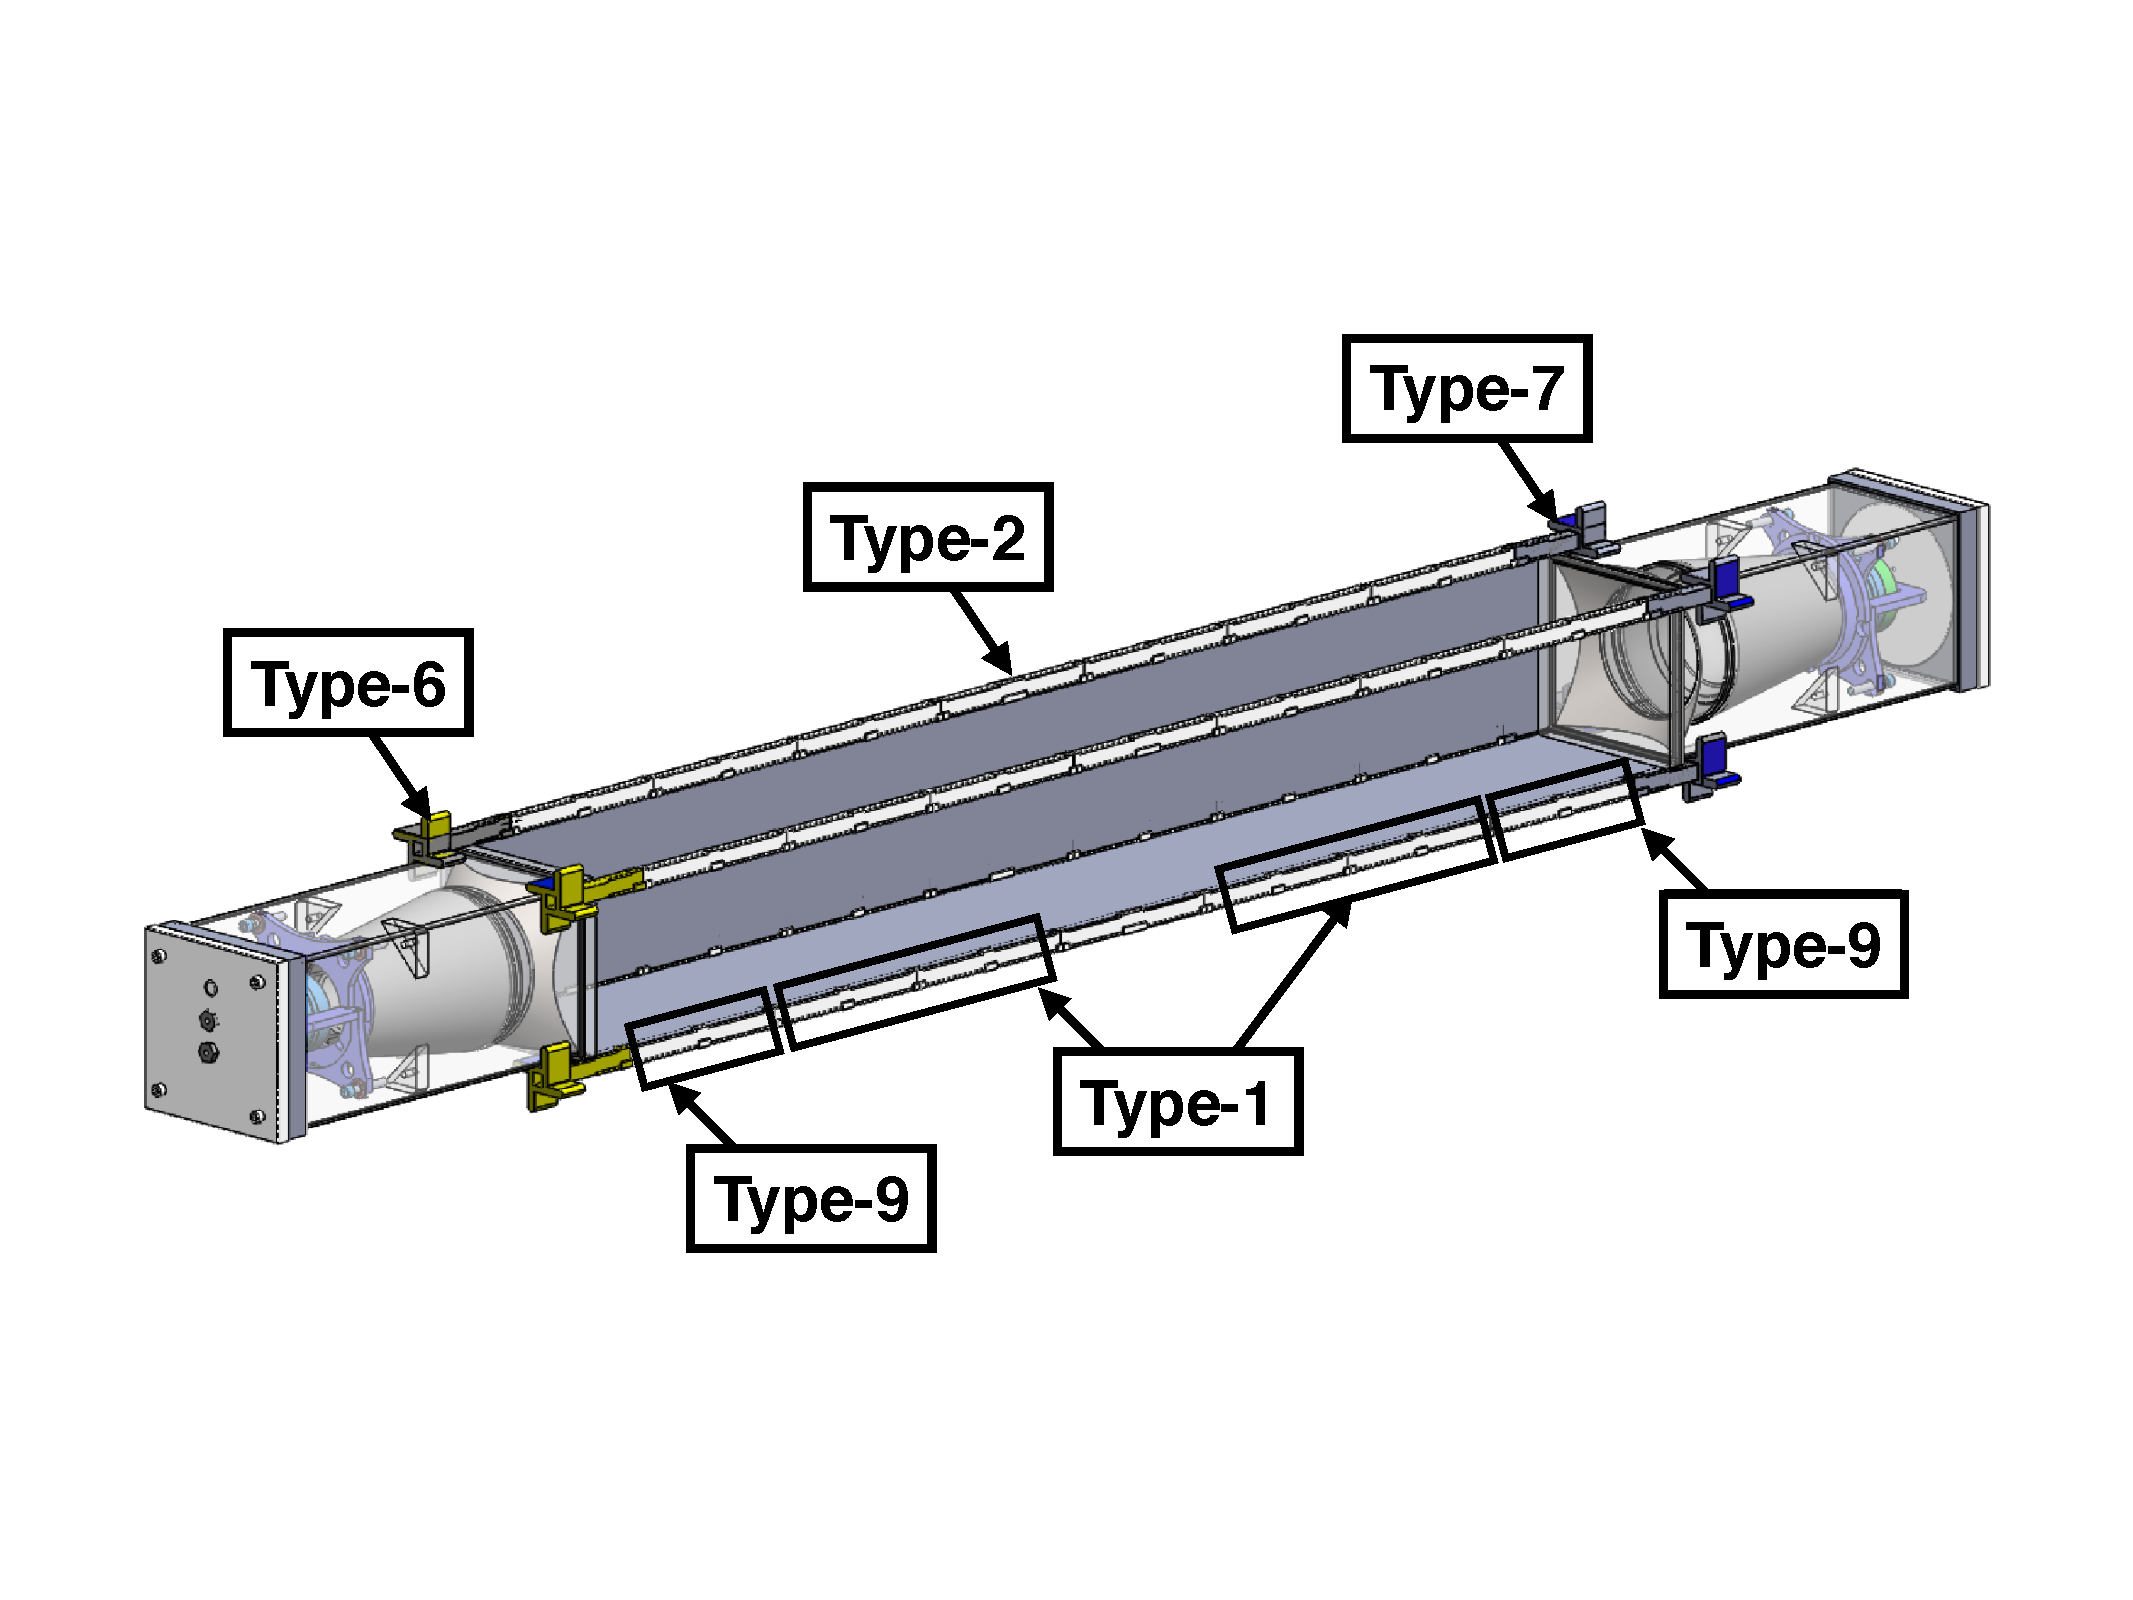
\includegraphics[trim = 0cm 5cm 0cm 5cm, clip,width=0.8\textwidth]{Figures/PinwheelLocation.pdf}
\caption[Assembled location of PLA rods]{The assembled locations of different types of PLA rods. In this figure, the end PLA rods are type-6 and -7. If a segment is at a corner of the detector, the end PLA rods at the specific corner of the segment would be type-4 and -5. Similarly, if the segment is on the edge of the detect, the end PLA rods on one edge would be type-3 and -8.}
\label{fig:pinwheelloc}
\end{figure}

There are 1620 PLA rods of different types needed for PROSPECT.
The PLA rods are 3D printed by a company specialized in commercial 3D printing with multiple 3D printers to parallel print all PLA rods.
According to the manufacturer, the PLA rods were printed with 100~\textmu m PLA filament.

Temperature instability during 3D printing can cause burnt spots on the PLA surface. 
Because the burnt PLA's compatibility with $^6$LiLS is unknown, PLA rods with burnt spots were rejected.
The surface quality of the PLA rods is evaluated in QA, for shape imperfection can cause a puncture to the separators' FEP film.
10-20\% of the PLA rods were rejected for burns, contributing the majority of the rejects. 
Hence, the surfaces of each PLA rods were filed with stainless steel files.  
The spacer volume was further filed through CNC machining to ensure precise dimensions required for accurate placement of end PLA rods between the PMT modules.

Before the assembly of the PROSPECT AD, the PLA rods were strung along a thin supporting acrylic rod, as shown in Figure~\ref{fig:pinwheelPreclean}.
The string of PLA rods was firstly assembled with the corresponding separators, then assembled into the detector.

\begin{figure}[h!]
\centering
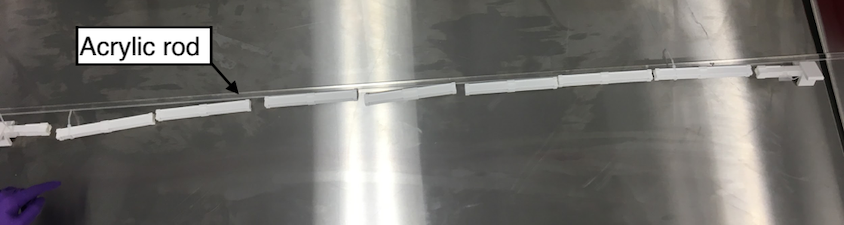
\includegraphics[width=0.7\textwidth]{Figures/PinwheelPreAssemble1.png}\\

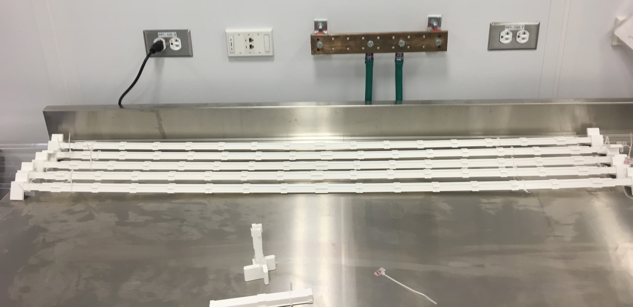
\includegraphics[width=0.7\textwidth]{Figures/PinwheelPreAssemble2.png}
\caption [Stringing of the PLA rods]{(Top) PLA rods and a acrylic rod before stringing. (Bottom) The pre-assembled long PLA rods strung on acrylic rods.}
\label{fig:pinwheelPreclean}
\end{figure}

\Subsection{Mass of the Optical Grid}
Comprehensive measurements of the optical grid components were made to quantify the key parameters that are important to validate the detector uniformity, stability, and provide quantities for PROSPECT's physics analysis.
The measured properties include mass and dimensions of the components, optical reflectance, and uniformity of the components, as well as material compatibility with the $^6$LiLS.

The mass of the separators was measured in batches during the optical grid assembly (see Section~\ref{sec:ad_construct}).
Every batch of separators assembled in the PROSPECT AD were weighed separately, and the average was calculated.
The PLA rods were weighed in randomly selected groups of 20 to 50 PLA rods, and the average mass was calculated.
Including the calibration system inserted into the the PLA rods, the total mass of the optical grid in the detector active volume is 134.8~kg $\pm$ 1.9~kg (158.1~kg with the calibration system and supporting acrylic rods), contributing $\sim3\%$ (3.5\% with PTFE tube and acrylic rods) of dead mass to the PROSPECT active target region.

\begin{table}[htpb]
\centering
\caption[Mass of the optical grid components]{The results of mass measurements on the separators and the PLA rods. 
All separators and PLA rods were weighed in batches and the quoted uncertainties reflect variation in the average component mass per batch.}
\begin{tabular}{p{5cm}ccc}
\hline
\hline
Category & Average mass(g) & Total amount & Total mass(kg)\\
\hline
Separator & $326\pm10$ & 333 & $108.7\pm1.7$\\
Standard PLA rod (type-1) & $12.3\pm0.1$ & 720 & $8.86\pm0.07$\\
Center PLA rod (type-2) & $12.8\pm0.2$ & 180 & $2.30\pm0.04$\\
Standard PLA rod (type-9) & $12.5\pm0.02$ & 360 & $4.50\pm0.07$\\
Four arms end PLA rod (type-6\&7)& $29.7\pm0.2$ & 260 & $7.72\pm0.05$ \\
Three arms end PLA rod (type-3\&8)& $26.8\pm0.1$ & 92 & $2.47\pm0.01$\\
Two arms end PLA rod (type-4\&5) & $20.8\pm0.1$ & 8 & 0.2\\
\hline
\end{tabular}

\label{tab:mass}
\end{table}

\Subsection{Dimensional Characterization of Optical Grid Components}
Exhaustive dimensional measurements were done on separators. 
The thickness of the separators is an essential dimension due to its correlation with particle energy loss in the dead volume of the PROSPECT AD.
Each separator was measured with a thickness gauge at 12 different locations on the separator. 
The results of the thickness measurements are shown in Figure~\ref{fig:panelMeasure}.
The average separator thickness is 1.18$\pm$0.05~mm.

\begin{figure}[h!]
\centering
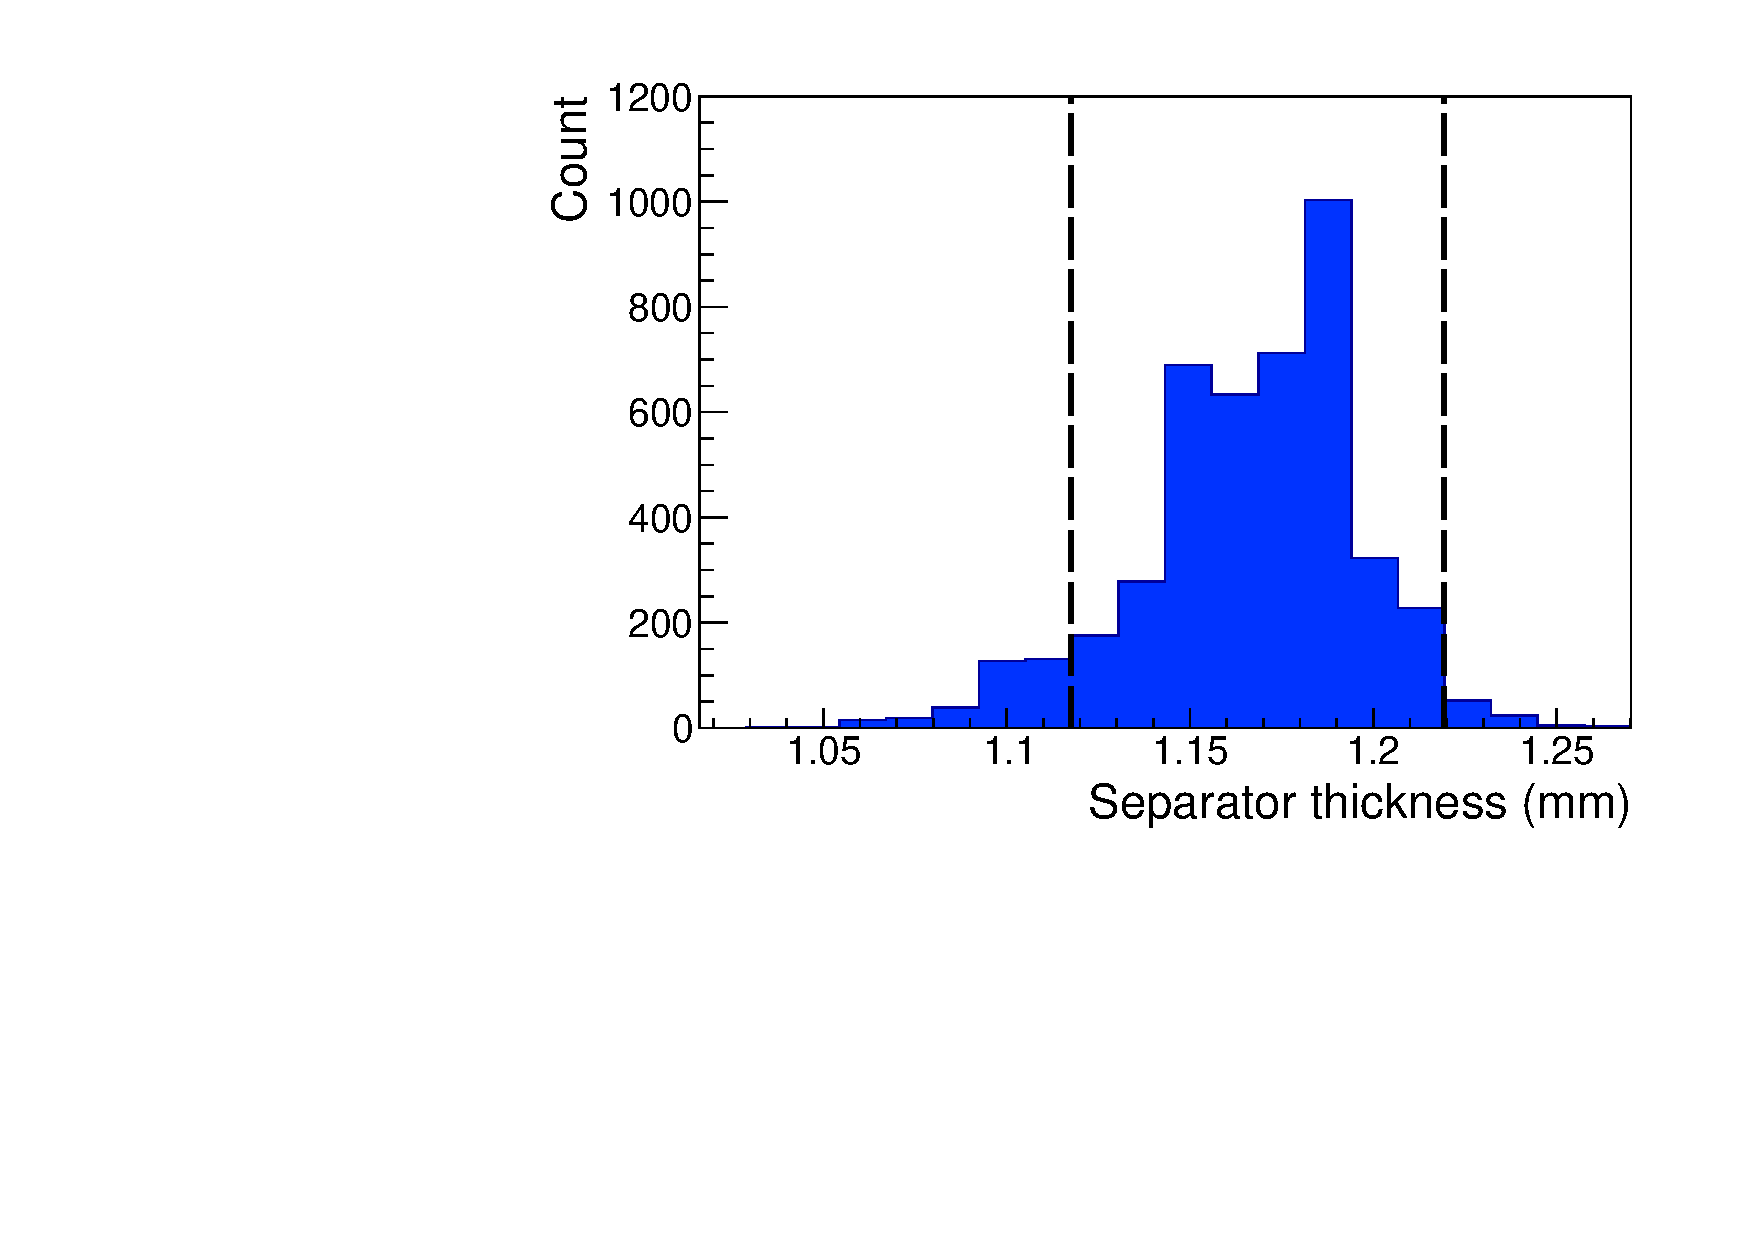
\includegraphics[width=0.48\textwidth]{Figures/PanelThick351.pdf}
\caption[Thickness of separators]{Thickness measurements made on 351 separators, where  the dashed line represents fabrication tolerances. }
\label{fig:panelMeasure}
\end{figure}

5\% of all produced PLA rods were measured to ensure their dimensional uniformity among batches of production.
Dimensional repeatability of 3D printing of PLA was demonstrated at the $\pm$0.13~mm level through the measurement.

\Subsection{Optical Performance of the Optical Grid}
The separator reflectance was measured with an Ocean Optics STS-VIS spectrometer to ensure optical uniformity.
The relative total reflectance (specular+diffuse) comparing to a smaller separator sample and the absolute diffuse reflectance were measured.
As shown in Figure~\ref{fig:Reflector}, the total reflectance of all separators varied within 2\%, and the diffuse reflectance was $<10\%$.

\begin{figure}[h!]
\centering
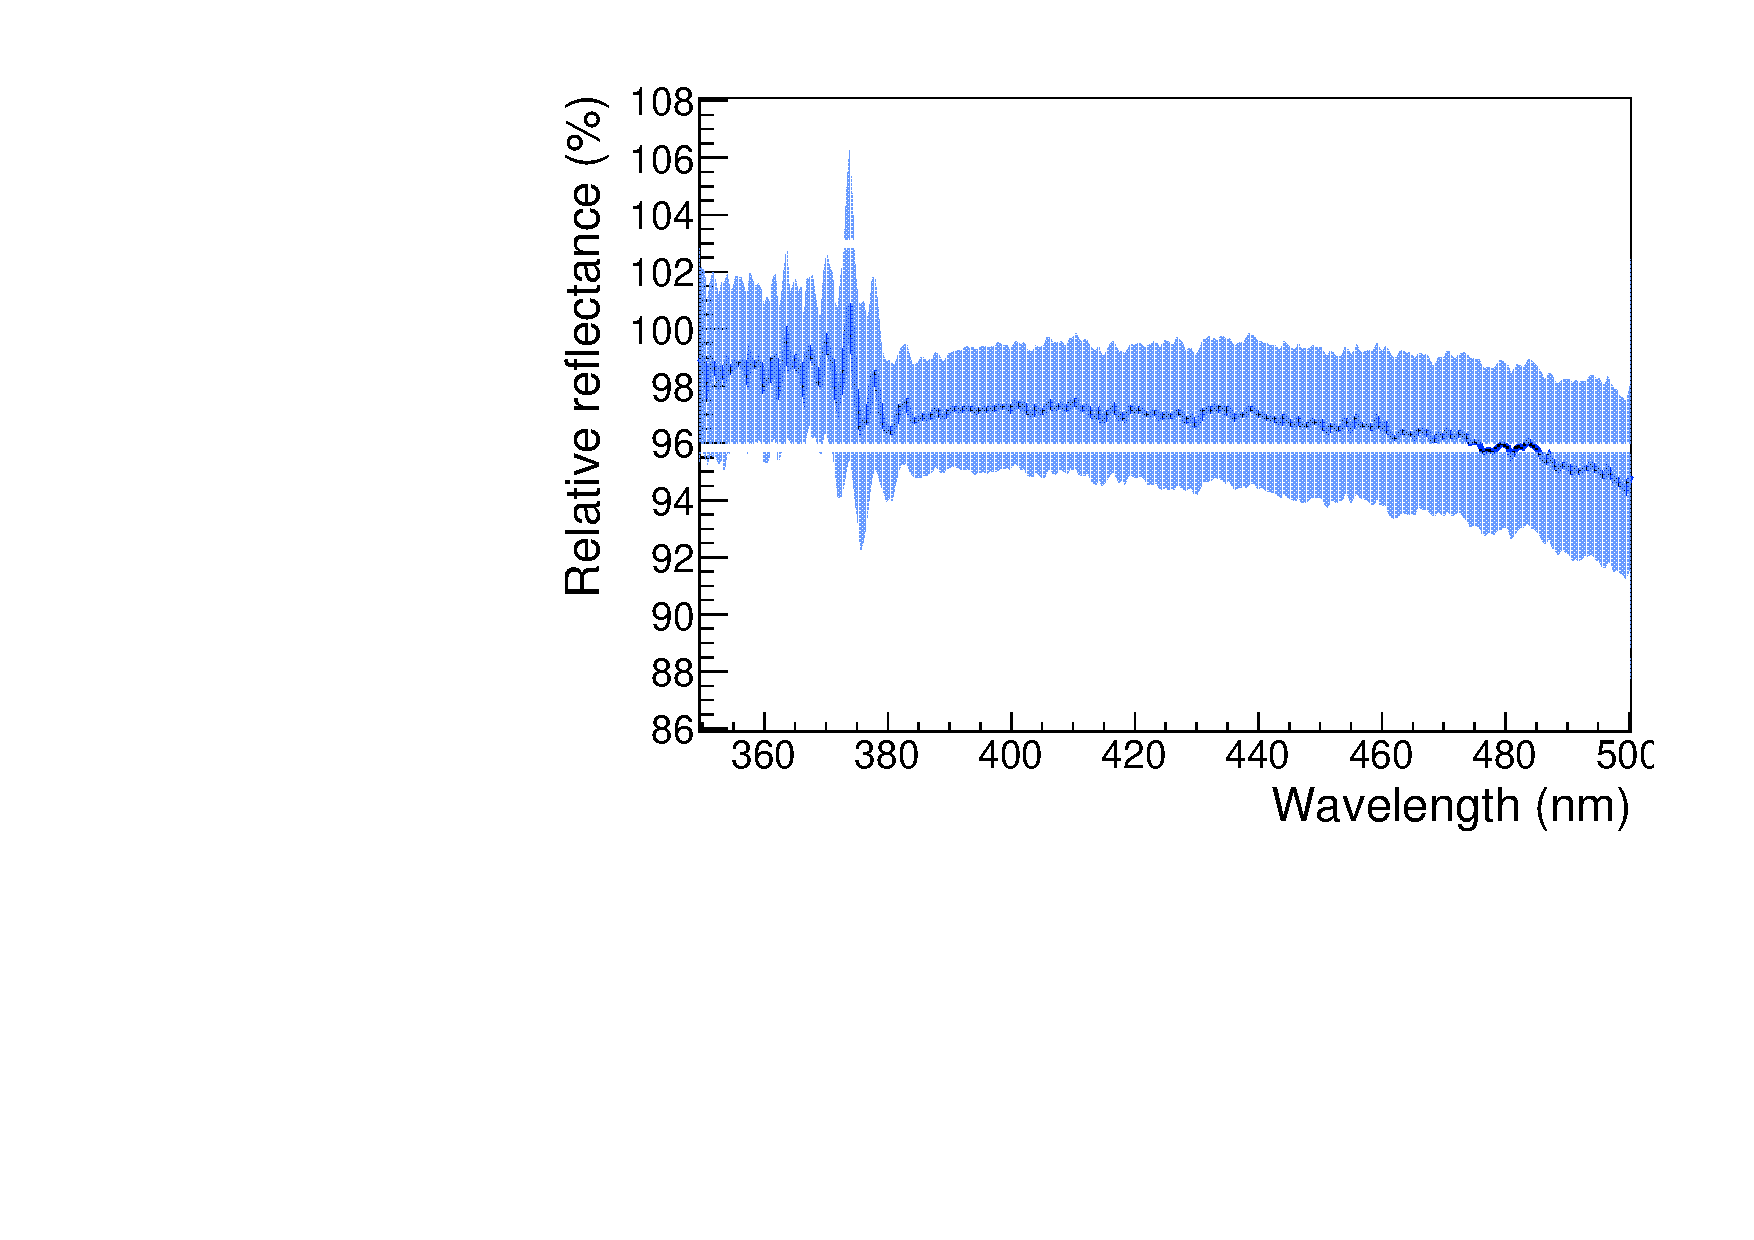
\includegraphics[width=.45\textwidth]{Figures/Panel_Spec.pdf}\quad
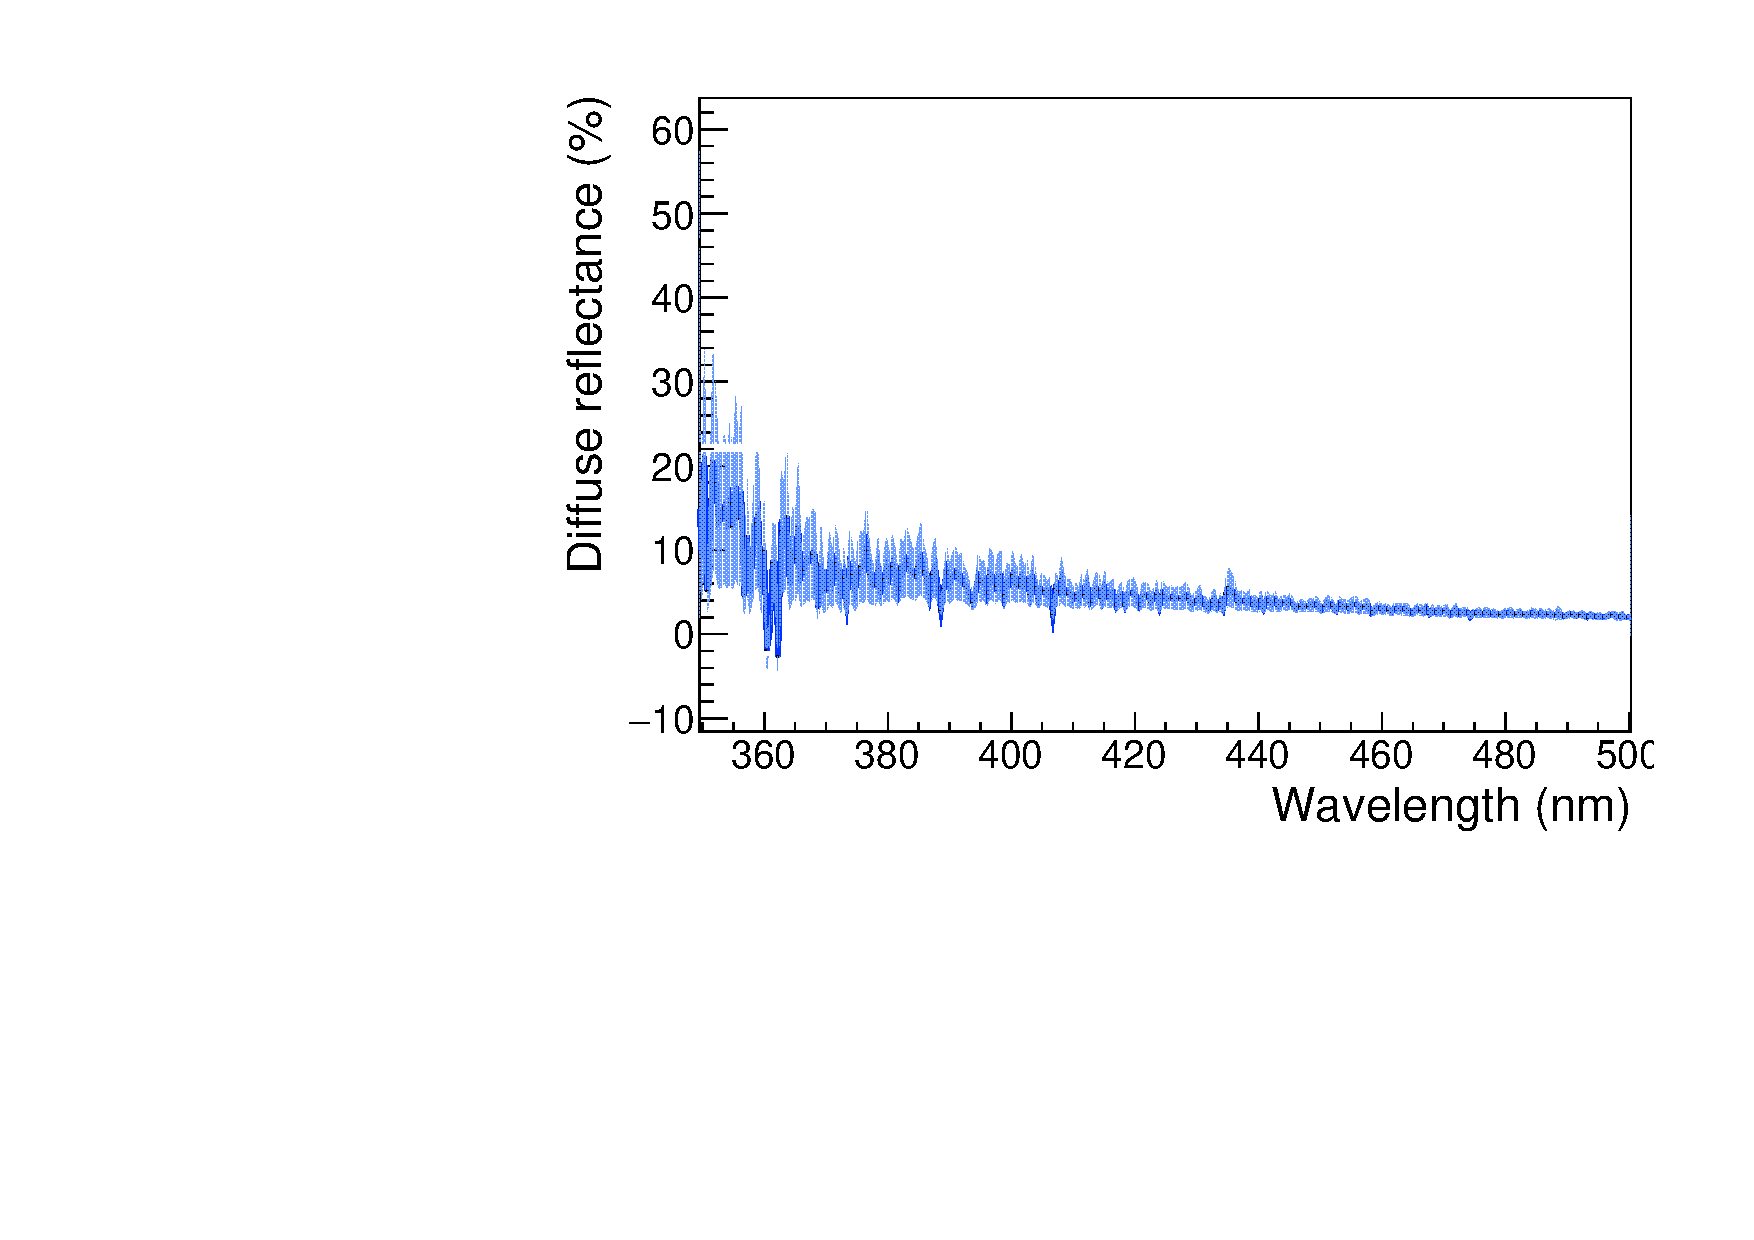
\includegraphics[width=.45\textwidth]{Figures/Panel_Diff.pdf}
\caption[Separator reflectance measurement]{
(Left) The relative reflectance of the mass production separators compared aganst a 5~cm $\times$ 5~cm separator sample with 1$\sigma$ error, showing 5\% of difference from the sample but $\pm$ 2\% variation among all separators. 
(Right) The diffuse reflectance of the mass production separators with 1$\sigma$ error, exhibiting $<10\%$ absolute diffuse reflectance.}
\label{fig:Reflector}
\end{figure}

The scintillation light reflects on the separator surface with random incident angle.
Ensuring reflectance uniformity with different incident angles of light is essential.
A laser goniometer was built at IIT to measure the correlation between reflectance and incident angle in EJ-309.
The result of the goniometer measurement is shown in Figure~\ref{fig:gonioreflect}. 
With increasing incident angle, the reflectance of bare DF2000MA decreases significantly in EJ-309 beyond $50^\circ$, while the reflectance of the separator remains flat because of the total internal reflection from the FEP film at large incident angles.

\begin{figure}[h!]
\centering
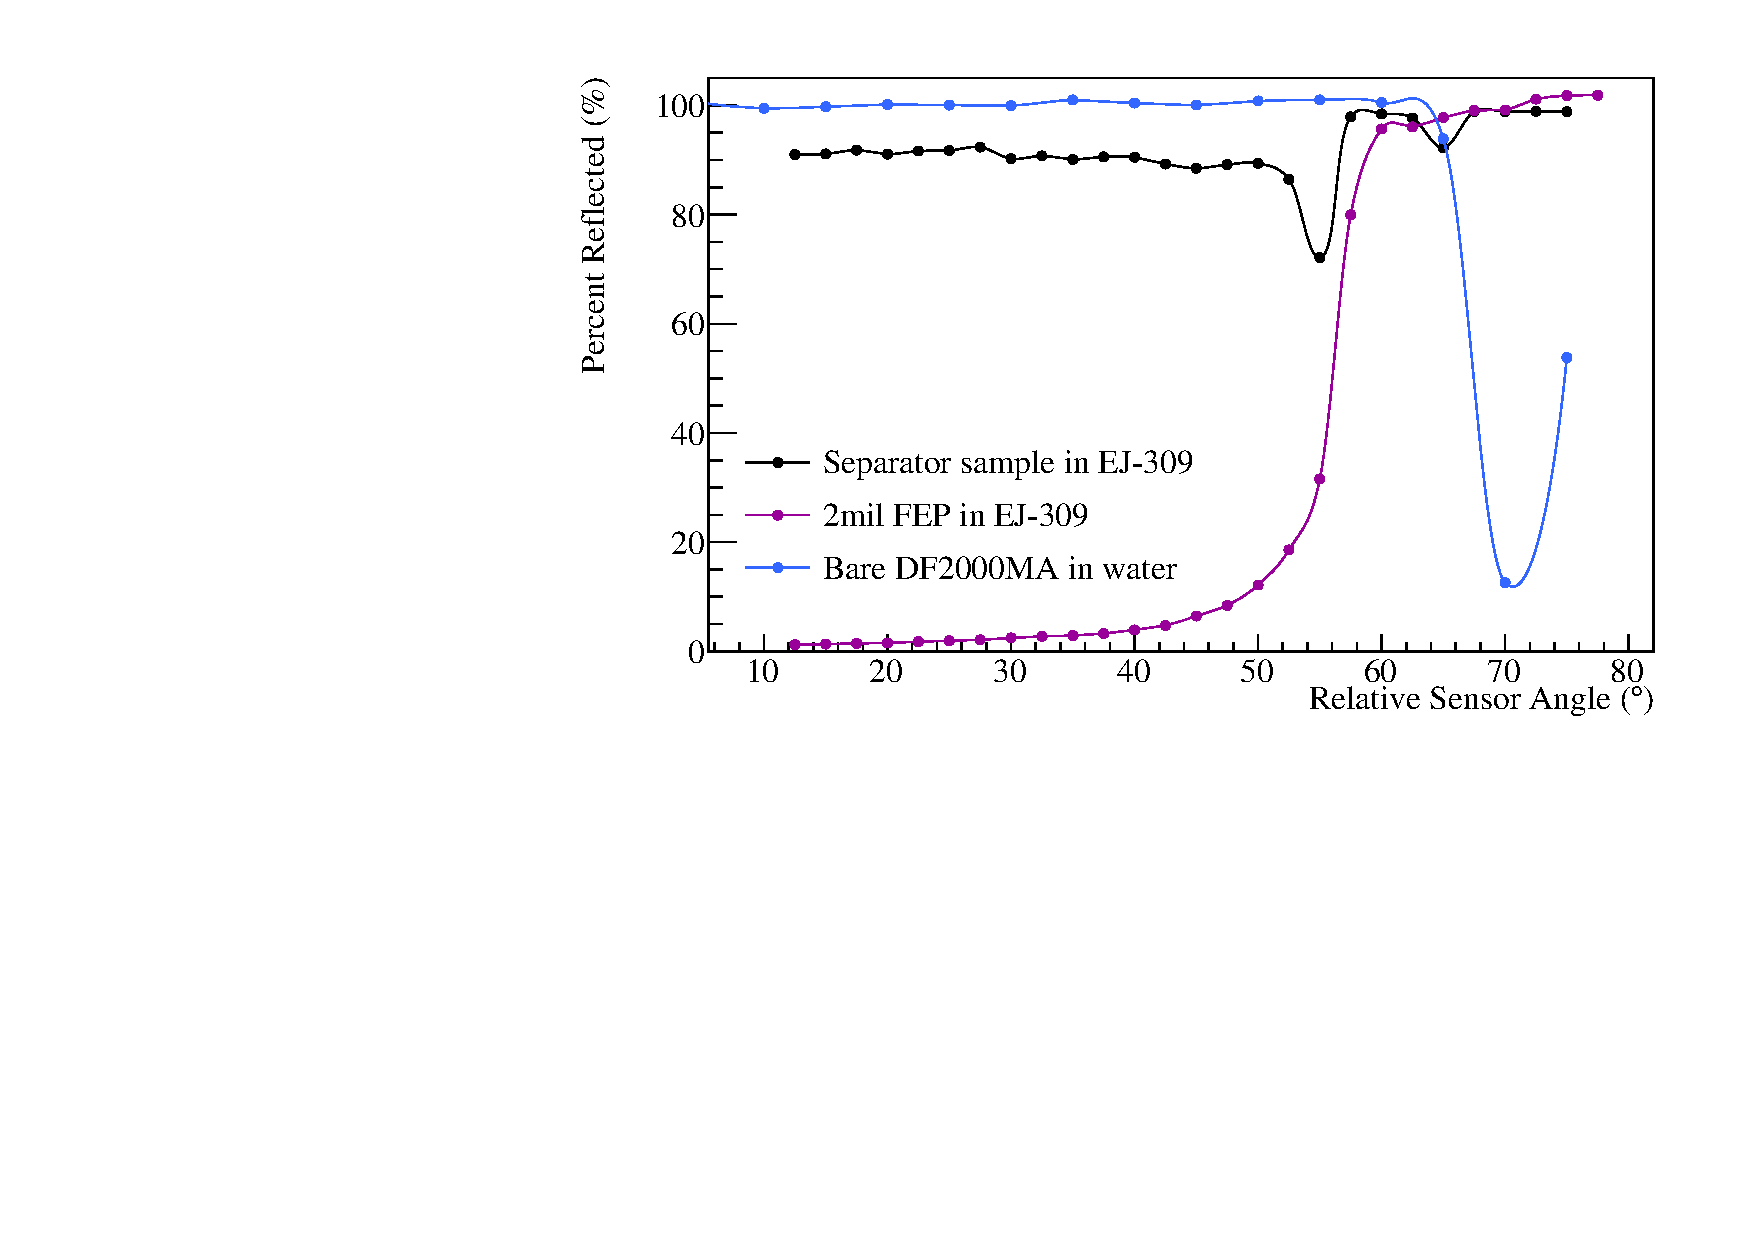
\includegraphics[width=0.49\textwidth]{Figures/DF2000specCompare.pdf}
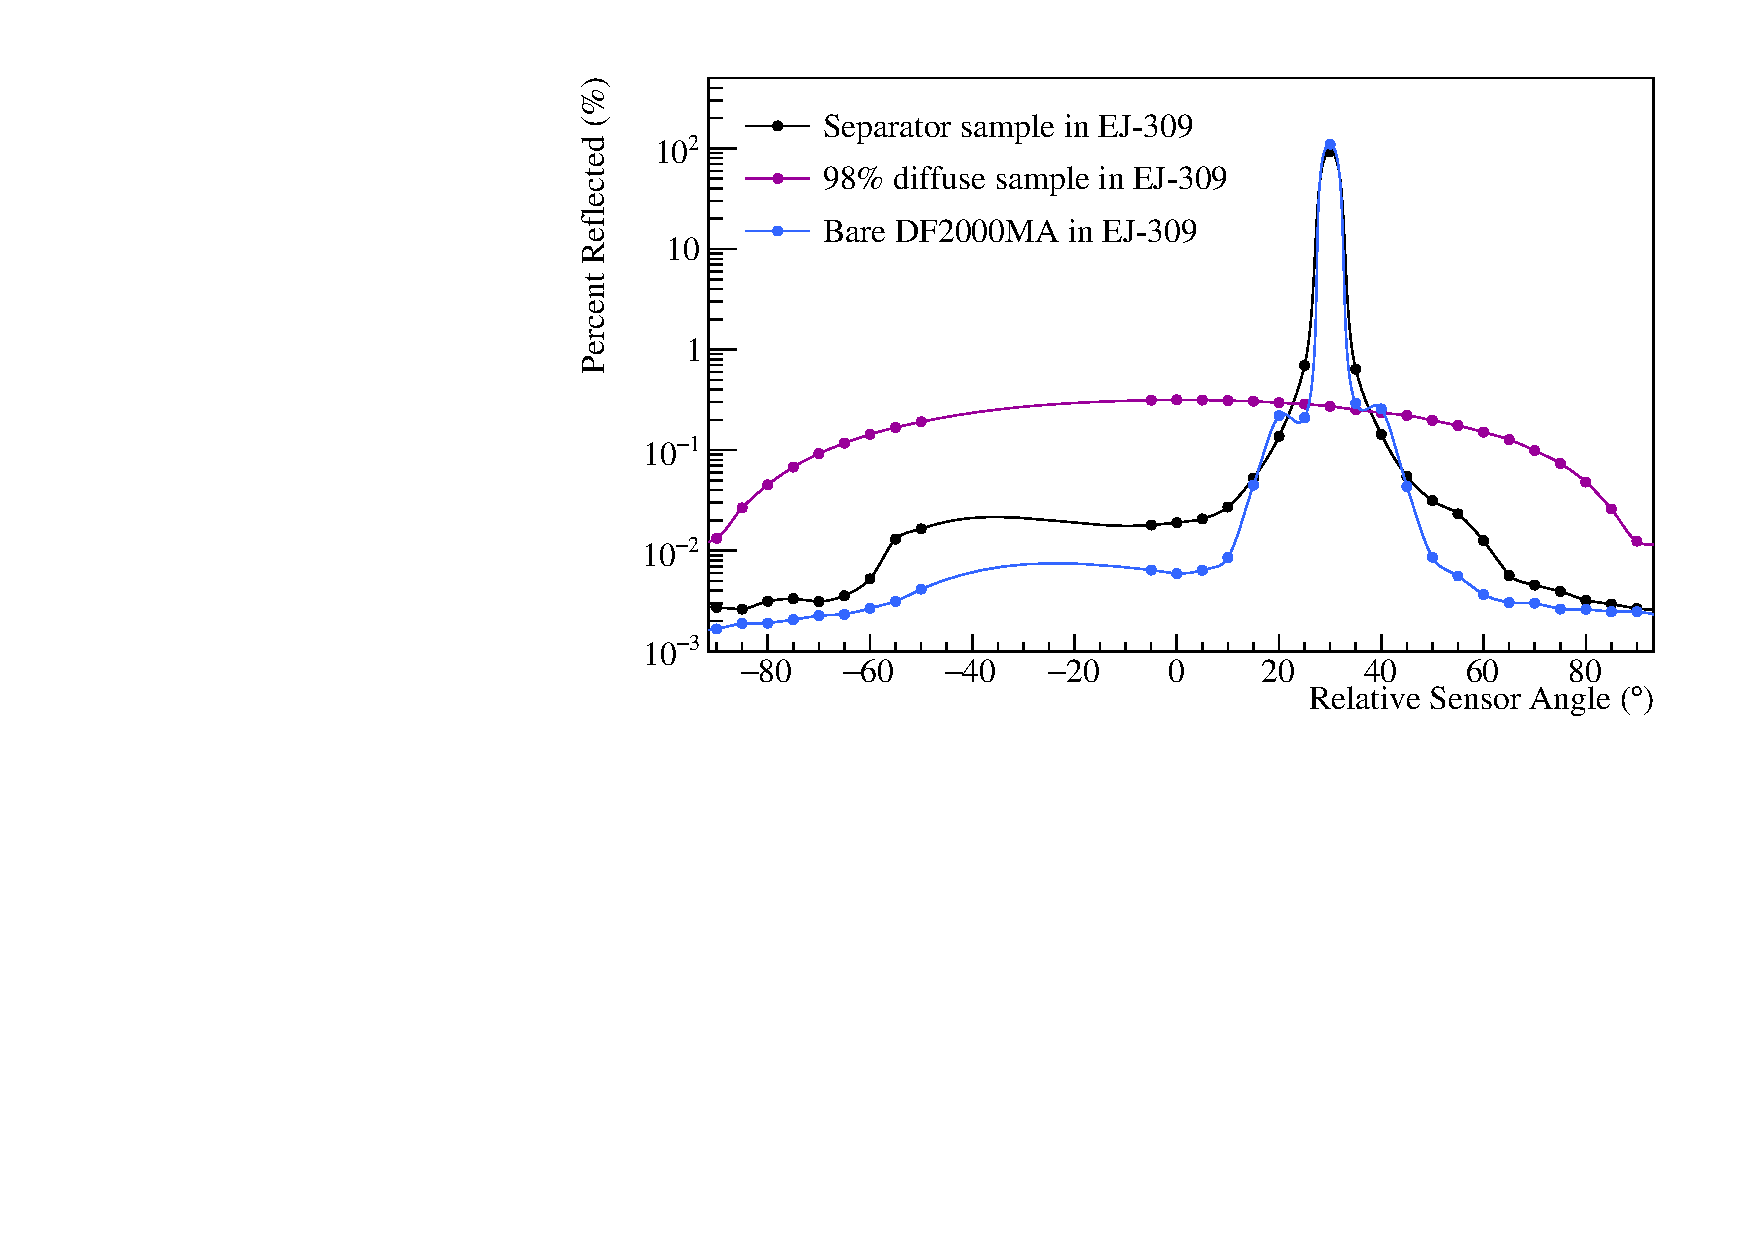
\includegraphics[width=0.49\textwidth]{Figures/DF2000diffCompare.pdf}
\caption[Results of the goniometer measurements]{The results of goniometer measurements on PROSPECT's separator sample. (Left) The specular reflectance of the laminated separator sample, FEP and bare DF2000MA in clear liquid, with respect to incident angle, shows the total internal reflection effect at large angle. (Right) The diffuse reflectance measured by the goniometer. The bare and laminated reflector compared against a 98\% diffuse reflective sample.}
\label{fig:gonioreflect}
\end{figure}

The optical characterization of PLA rods is shown in Figure~\ref{fig:PinwheelOptic}.
The light reflection of the PLA rods is dominated by diffuse reflection, with 65\% to 75\% absolute diffuse reflectance.
Comparing to the separator, the specular reflectance of the PLA rods is 2\% to 3\%.
By comparing the reflectance of PLA backed by reflector and light trap, the light transmitted through a wall PLA rod is $<1\%$.

\Subsection{Optical Grid Compatibility}
The compatibility of the separator and PLA rods with $^6$LiLS were tested by long term $^6$LiLS quality monitoring.
Samples of the separators and PLA rods were soaked in $^6$LiLS.
When testing compatibility, the $^6$LiLS contacted by each material was subjected to light absorbance spectroscopic measurements with an Agilent Technologies Cary 5000 UV-Vis-NIR spectrometer. 
Incompatible material can cause a change in the absorbance spectrum of $^6$LiLS, comparing to a reference $^6$LiLS sample.
The result of 6-month-long monitoring measurements are shown in Figure~\ref{fig:compat}, indicating no significant change in the absorbance spectrum comparing to the reference.

\begin{figure}[h!]
\centering
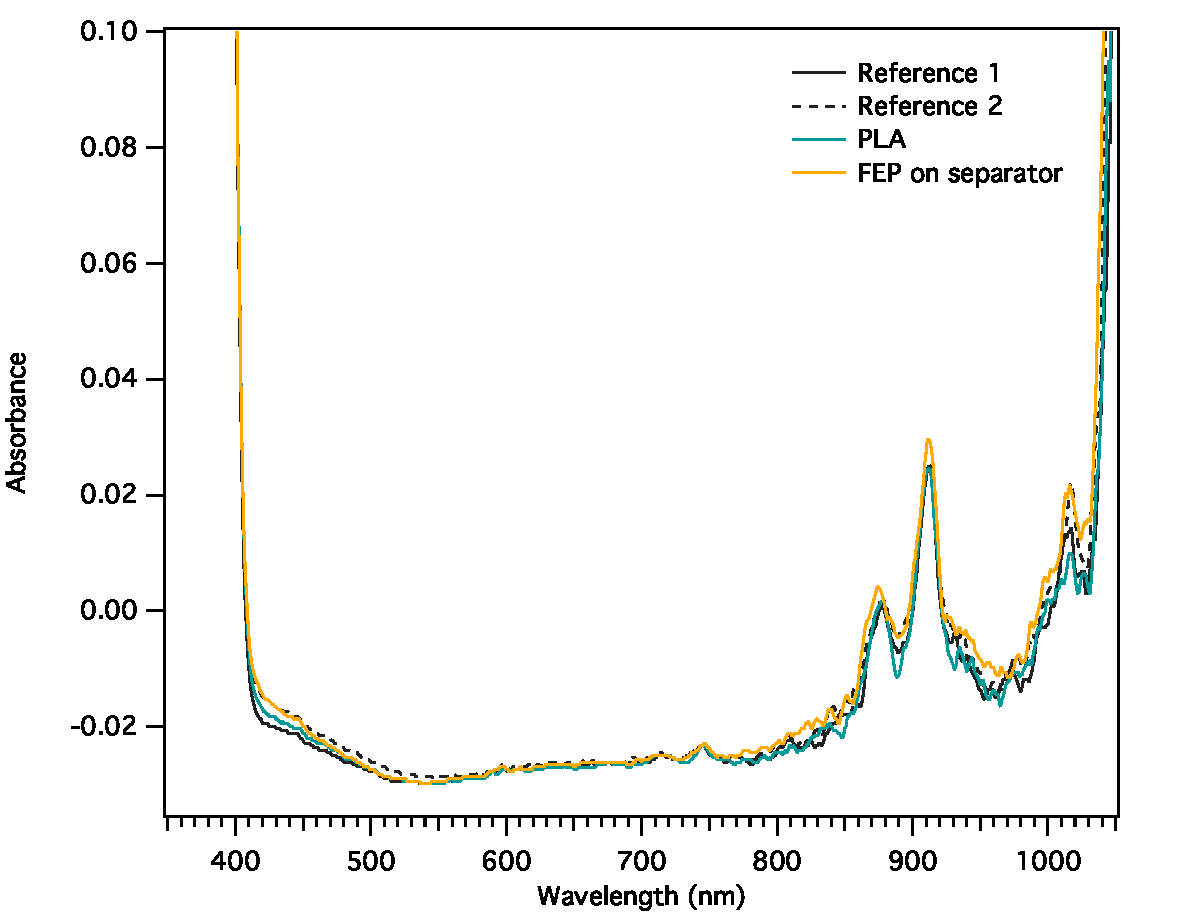
\includegraphics[width=.7\textwidth]{Figures/Fig28_a.pdf}
\caption[Optical grid compatibility]{The absorbance spectra of $^{6}$LiLS in contact with selected samples. 
After 6 months of contact with different detector components, all test liquid samples showed similar absorbance spectra compared with references.}
\label{fig:compat}
\end{figure}

The PLA rod mechanical stability while in contact with $^6$LiLS is also tested by a stressed lever test as shown in Figure~\ref{fig:leverPic}.
A 100~kPa stress is precisely applied to the PLA rod at the fulcrum by adjusting the weight and lever arm length.
The applied stress was calculated with an assumption of a square-shaped PLA rod cross-section.
EJ-309 was dropped at the fulcrum to maintain constant contact with PLA rod at the stressed spot.
In the 14-month-long lever test, the PLA rods with and without EJ-309 exposure remain straight, demonstrating PLA rods' mechanical stability.

\begin{figure}[h!]
\centering
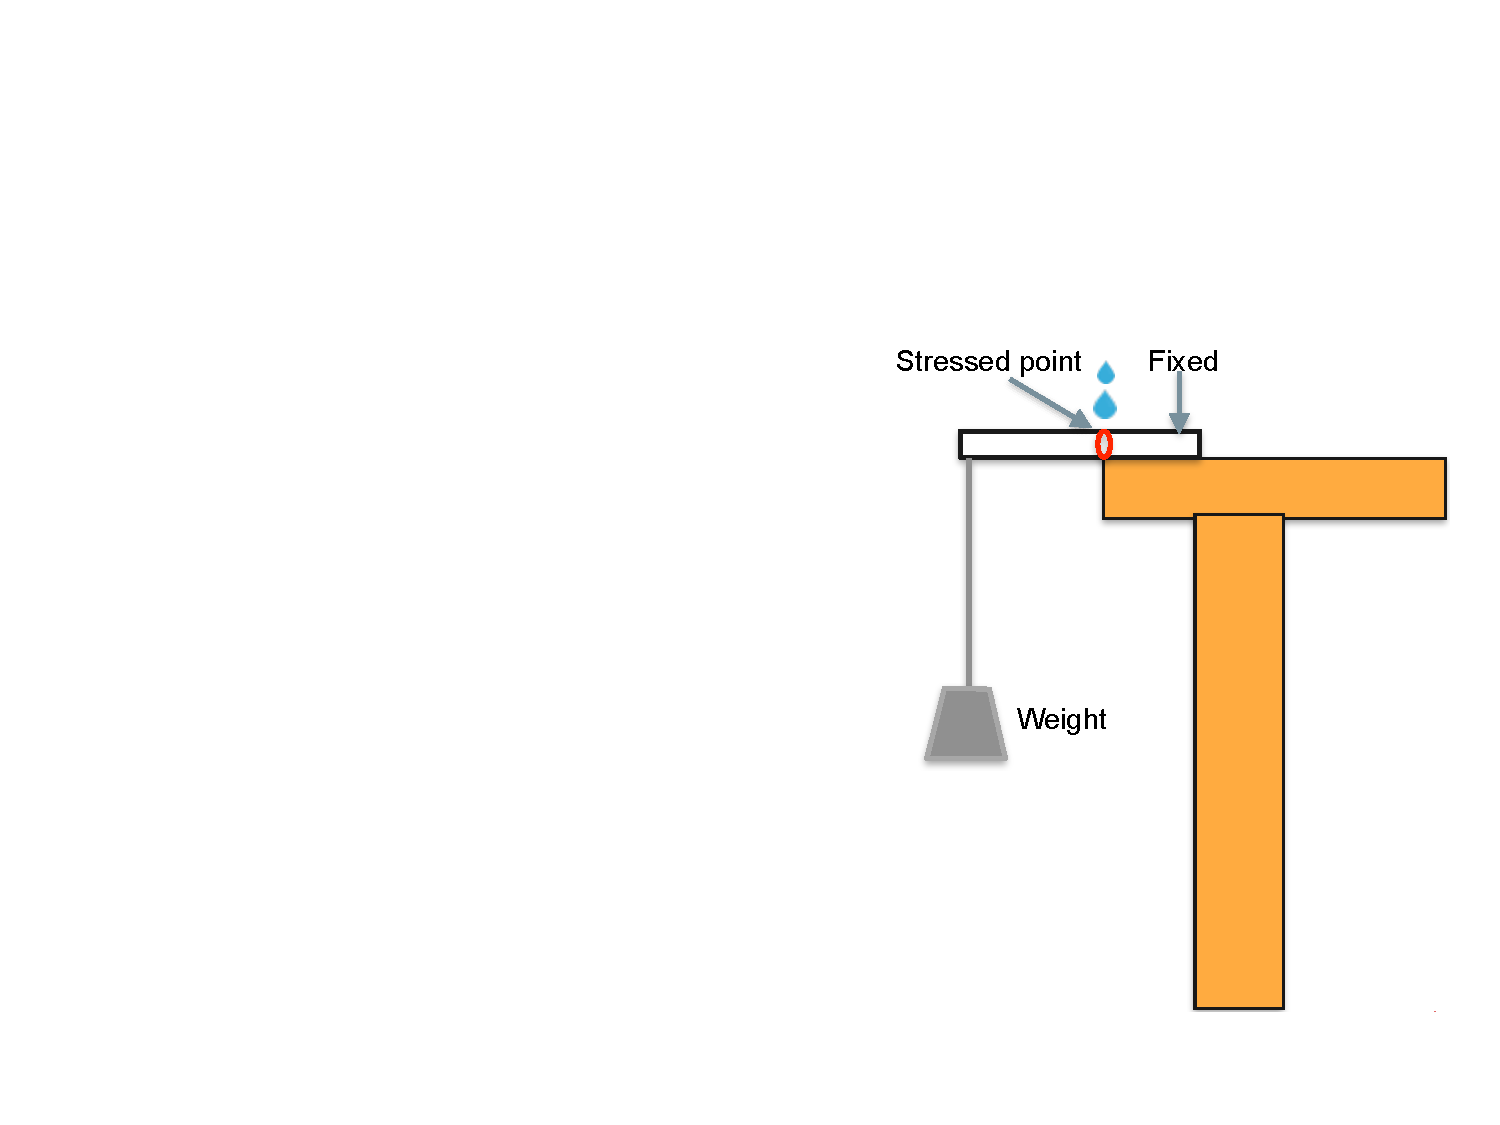
\includegraphics[width=0.45\textwidth]{Figures/StressScheme.pdf}
\caption[A schematic of PLA rod lever test]{A schematic of the lever test, where the liquid drops represent $^{6}$LiLS.}
\label{fig:leverPic}
\end{figure}

\Section{PMT Modules}

As mentioned in Figure~\ref{fig:active_volume}, PROSPECT utilizes two types of PMTs with 12.7~cm diameters and similar characteristics, including 240 Hamamatsu R6594 SEL PMTs and 68 ADIT ElectronTubes 9372KB PMTs.
To avoid light leakage and cross-talk among segments, the PMT module was designed with the purpose of creating light-tight segments within the optical grid.
Therefore, all PMTs are contained in the PMT housing shown in Figure~\ref{fig:pmtmodule} so that the PMT modules can be assembled inside the detector inner volume and submerged in $^6$LiLS.
The front window, sidewalls, and back plugs of the PMT housing are transparent, white-dyed, and black-dyed acrylic, respectively.
Each housing is filled with optically clear mineral oil to minimize the pressure difference between the inside and outside of the housing.
A 150~cc gas-filled bag inside the housing dampens any pressure variations due to thermal expansions.
The mineral oil and conical reflectors on the interior surface at the front window compose a light guide portion of the segment to increase light collection.
The dimensions of the sidewall are designed to fit precisely with the spacers of the end PLA rods. 
The back plugs of the PMT housings stack directly on each other in the PROSPECT AD. 
Hence, the segment dimension and variation is dependent on the dimension of PMT housings.
The front windows of the PMT housings are by design not contacting the optical grid, but have approximately 1~mm gap between them and separators to allow for filling of $^6$LiLS into the segments.
The back plug and cables were assembled into the module with O-rings for achieving the liquid-tight condition. 
All PMT modules were assembled in a class 1000 cleanroom at Yale University.

\begin{figure}[h!]
\centering
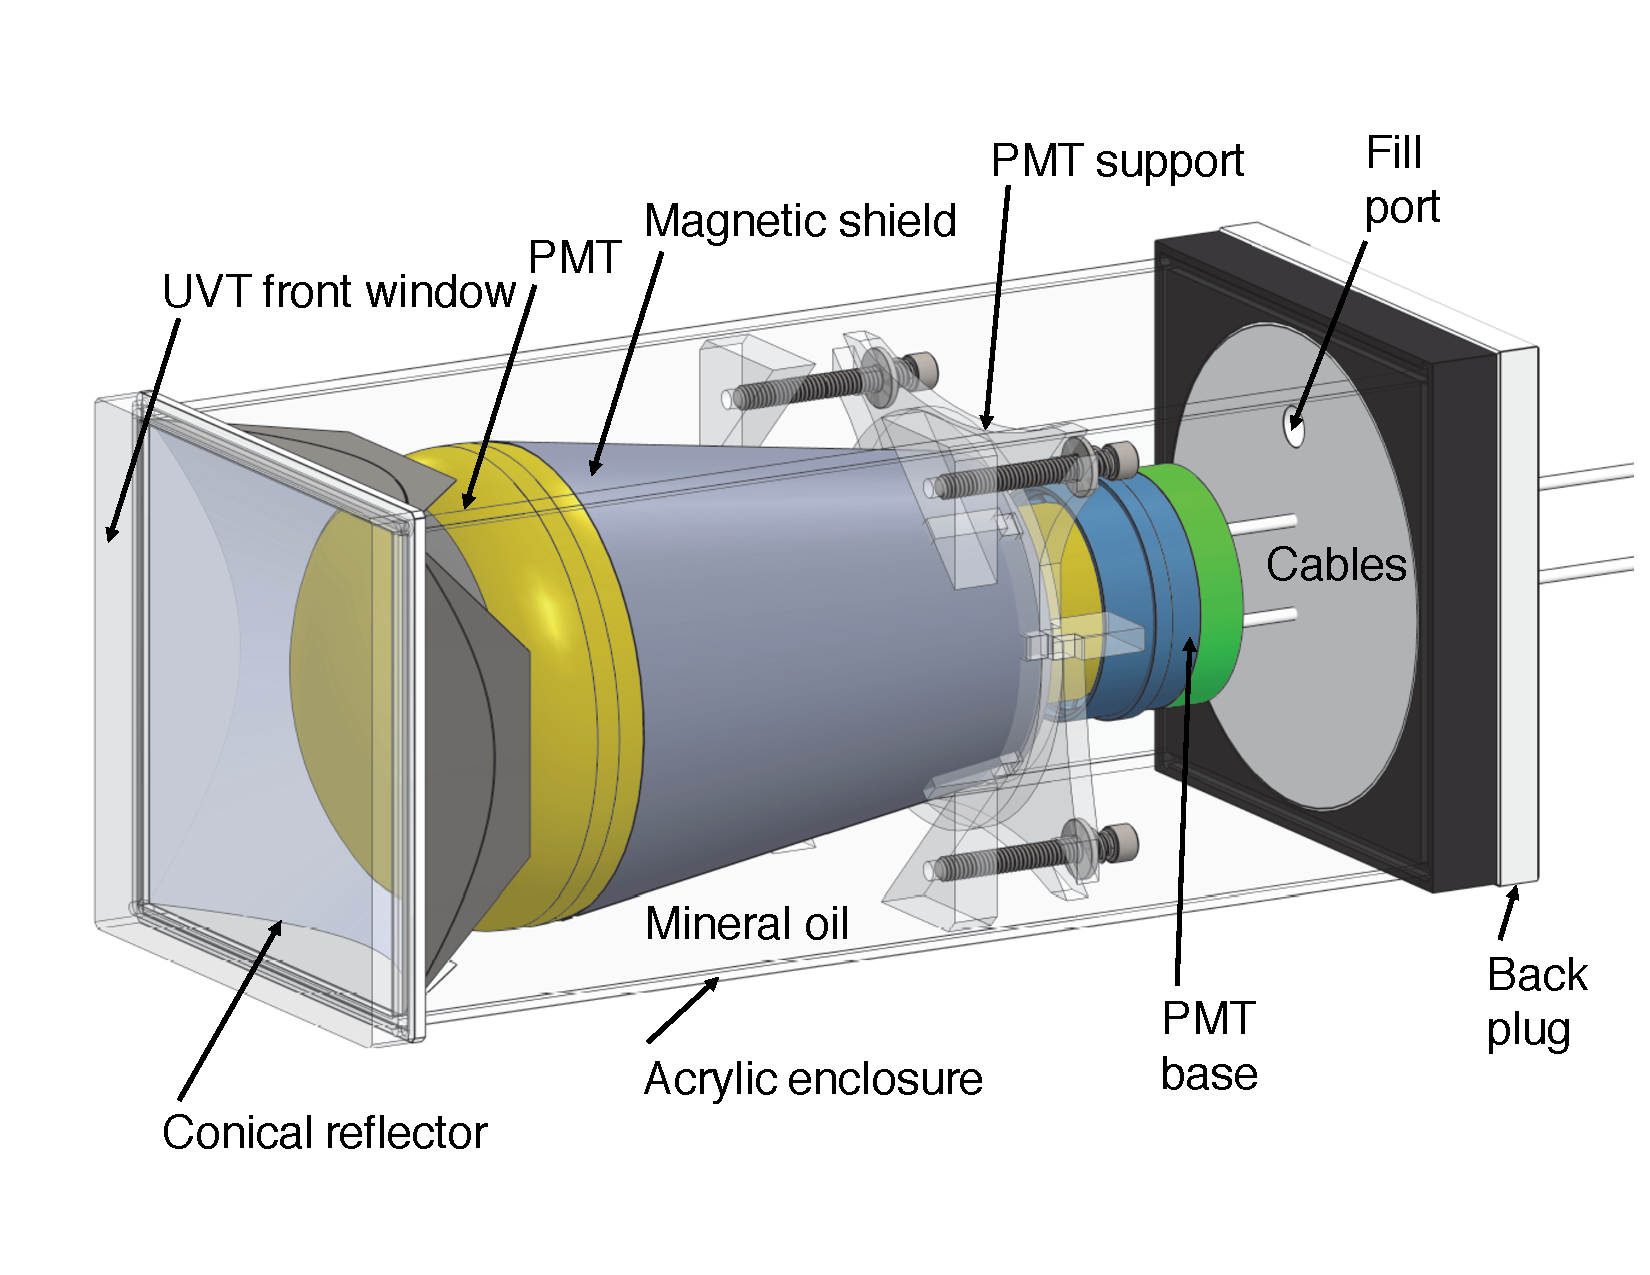
\includegraphics[width=0.6\textwidth]{Figures/PMTModule.pdf}
\caption[Design of the PMT modules]{The detailed design of the PMT module.}
\label{fig:pmtmodule}
\end{figure}

The mass and volume of the PMT modules after filling of mineral oil were measured.
Excluding cables, the mass of each Hamamatsu PMT module is 5.78$\pm$0.12~kg and the mass of each ElectronTubes module 5.49$\pm$0.12~kg.
The volume of each PMT housing is 6.6$\pm$0.3~liter. 

All PMT modules were subjected to PMT resistance tests and functionality tests before being assembled into the PROSPECT AD.
The PMT resistance was measured with multimeters during assembly.
In PMT functionality tests, groups of 16 fully assembled PMT modules were placed in a dark box where a laser-pulse LED  was deployed as a light source.
The PMT modules collected single photoelectron (PE) data with a variety of high voltage (HV) applied.
PMT modules with abnormal light response were re-assembled or rejected.

\Section{Calibration System}

The calibration system of PROSPECT consists of the $^{227}$Ac spiked in the $^6$LiLS (see Section~\ref{sec:LiLS}), optical calibration systems (OCS) inserted in the detector through some of the PLA rods, and radioactive source calibration systems~\cite{bib:prospect_calib}.
The schematic of the OCS and the radioactive source calibration setup is shown in Figure~\ref{fig:calibsystem}.

\begin{figure}[h!]
\centering
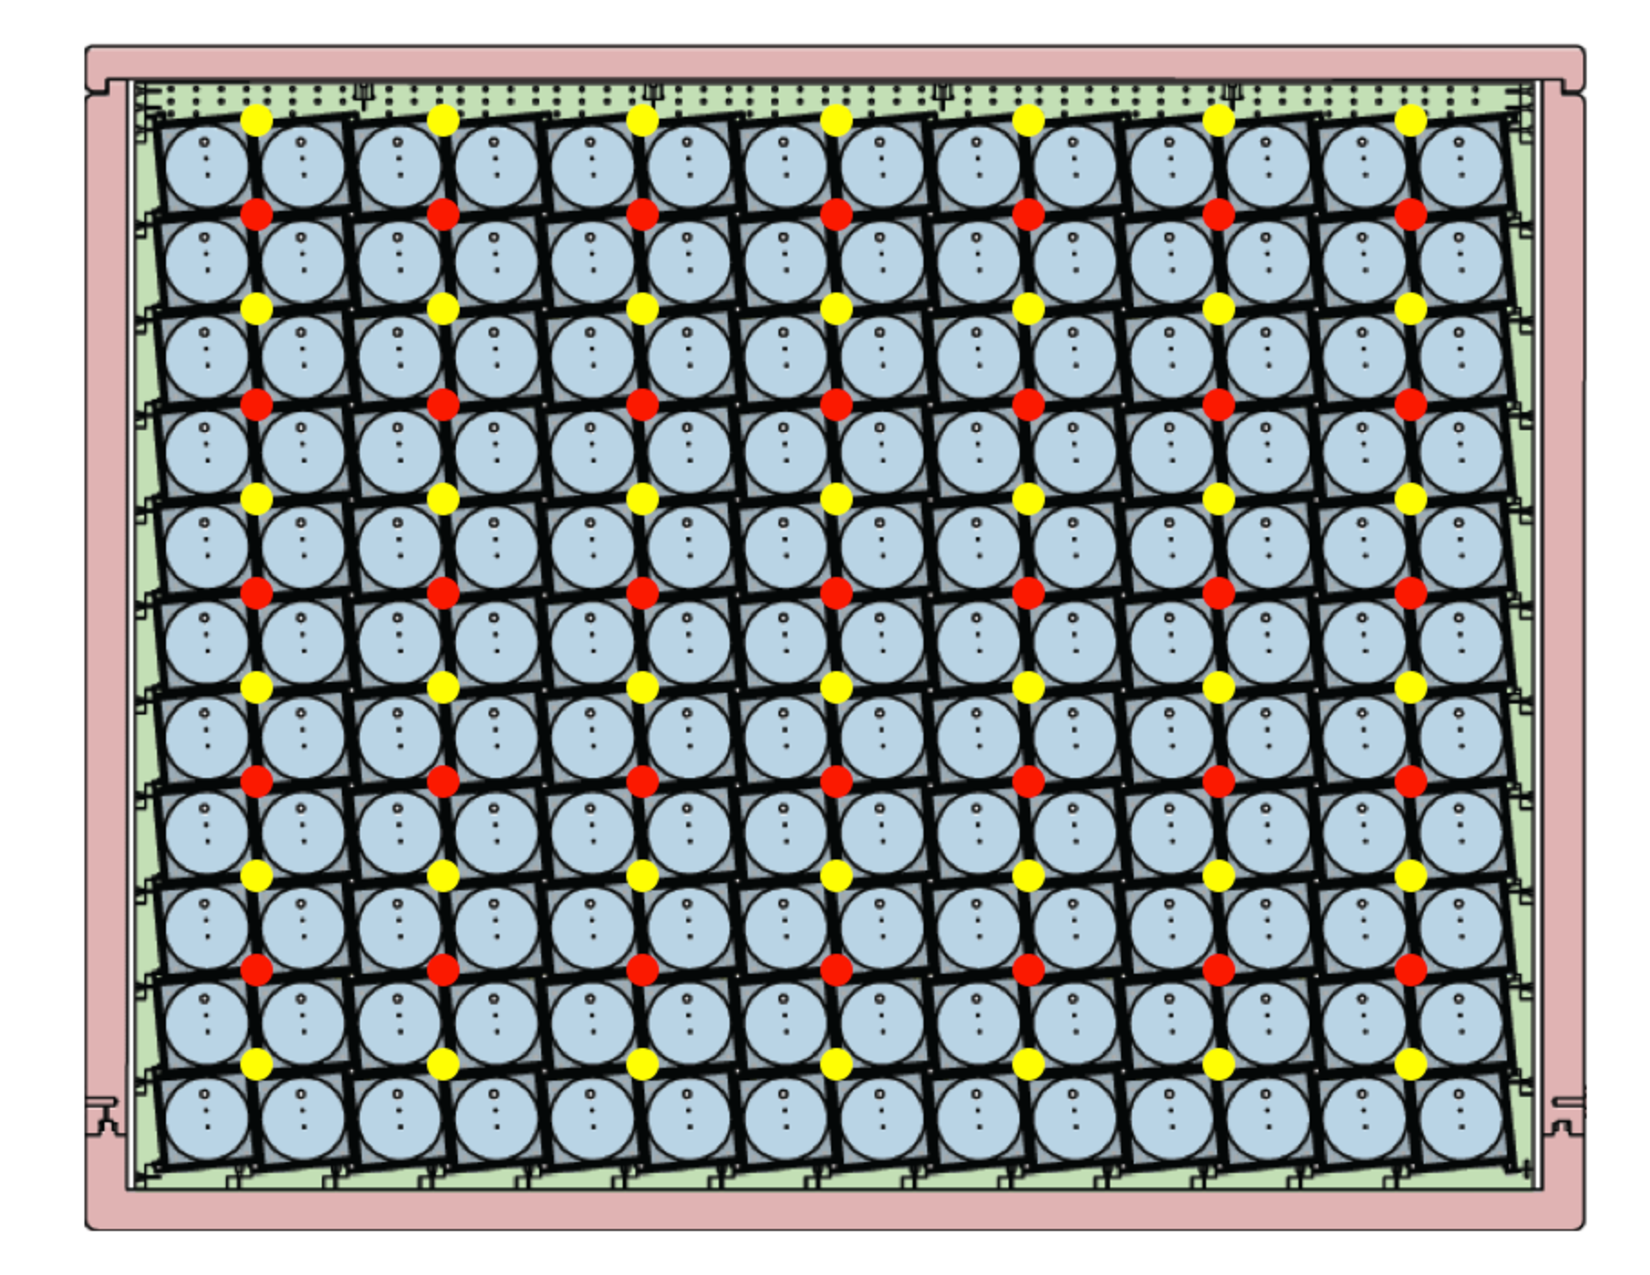
\includegraphics[width=0.6\textwidth]{Figures/CalibXY.pdf} \\
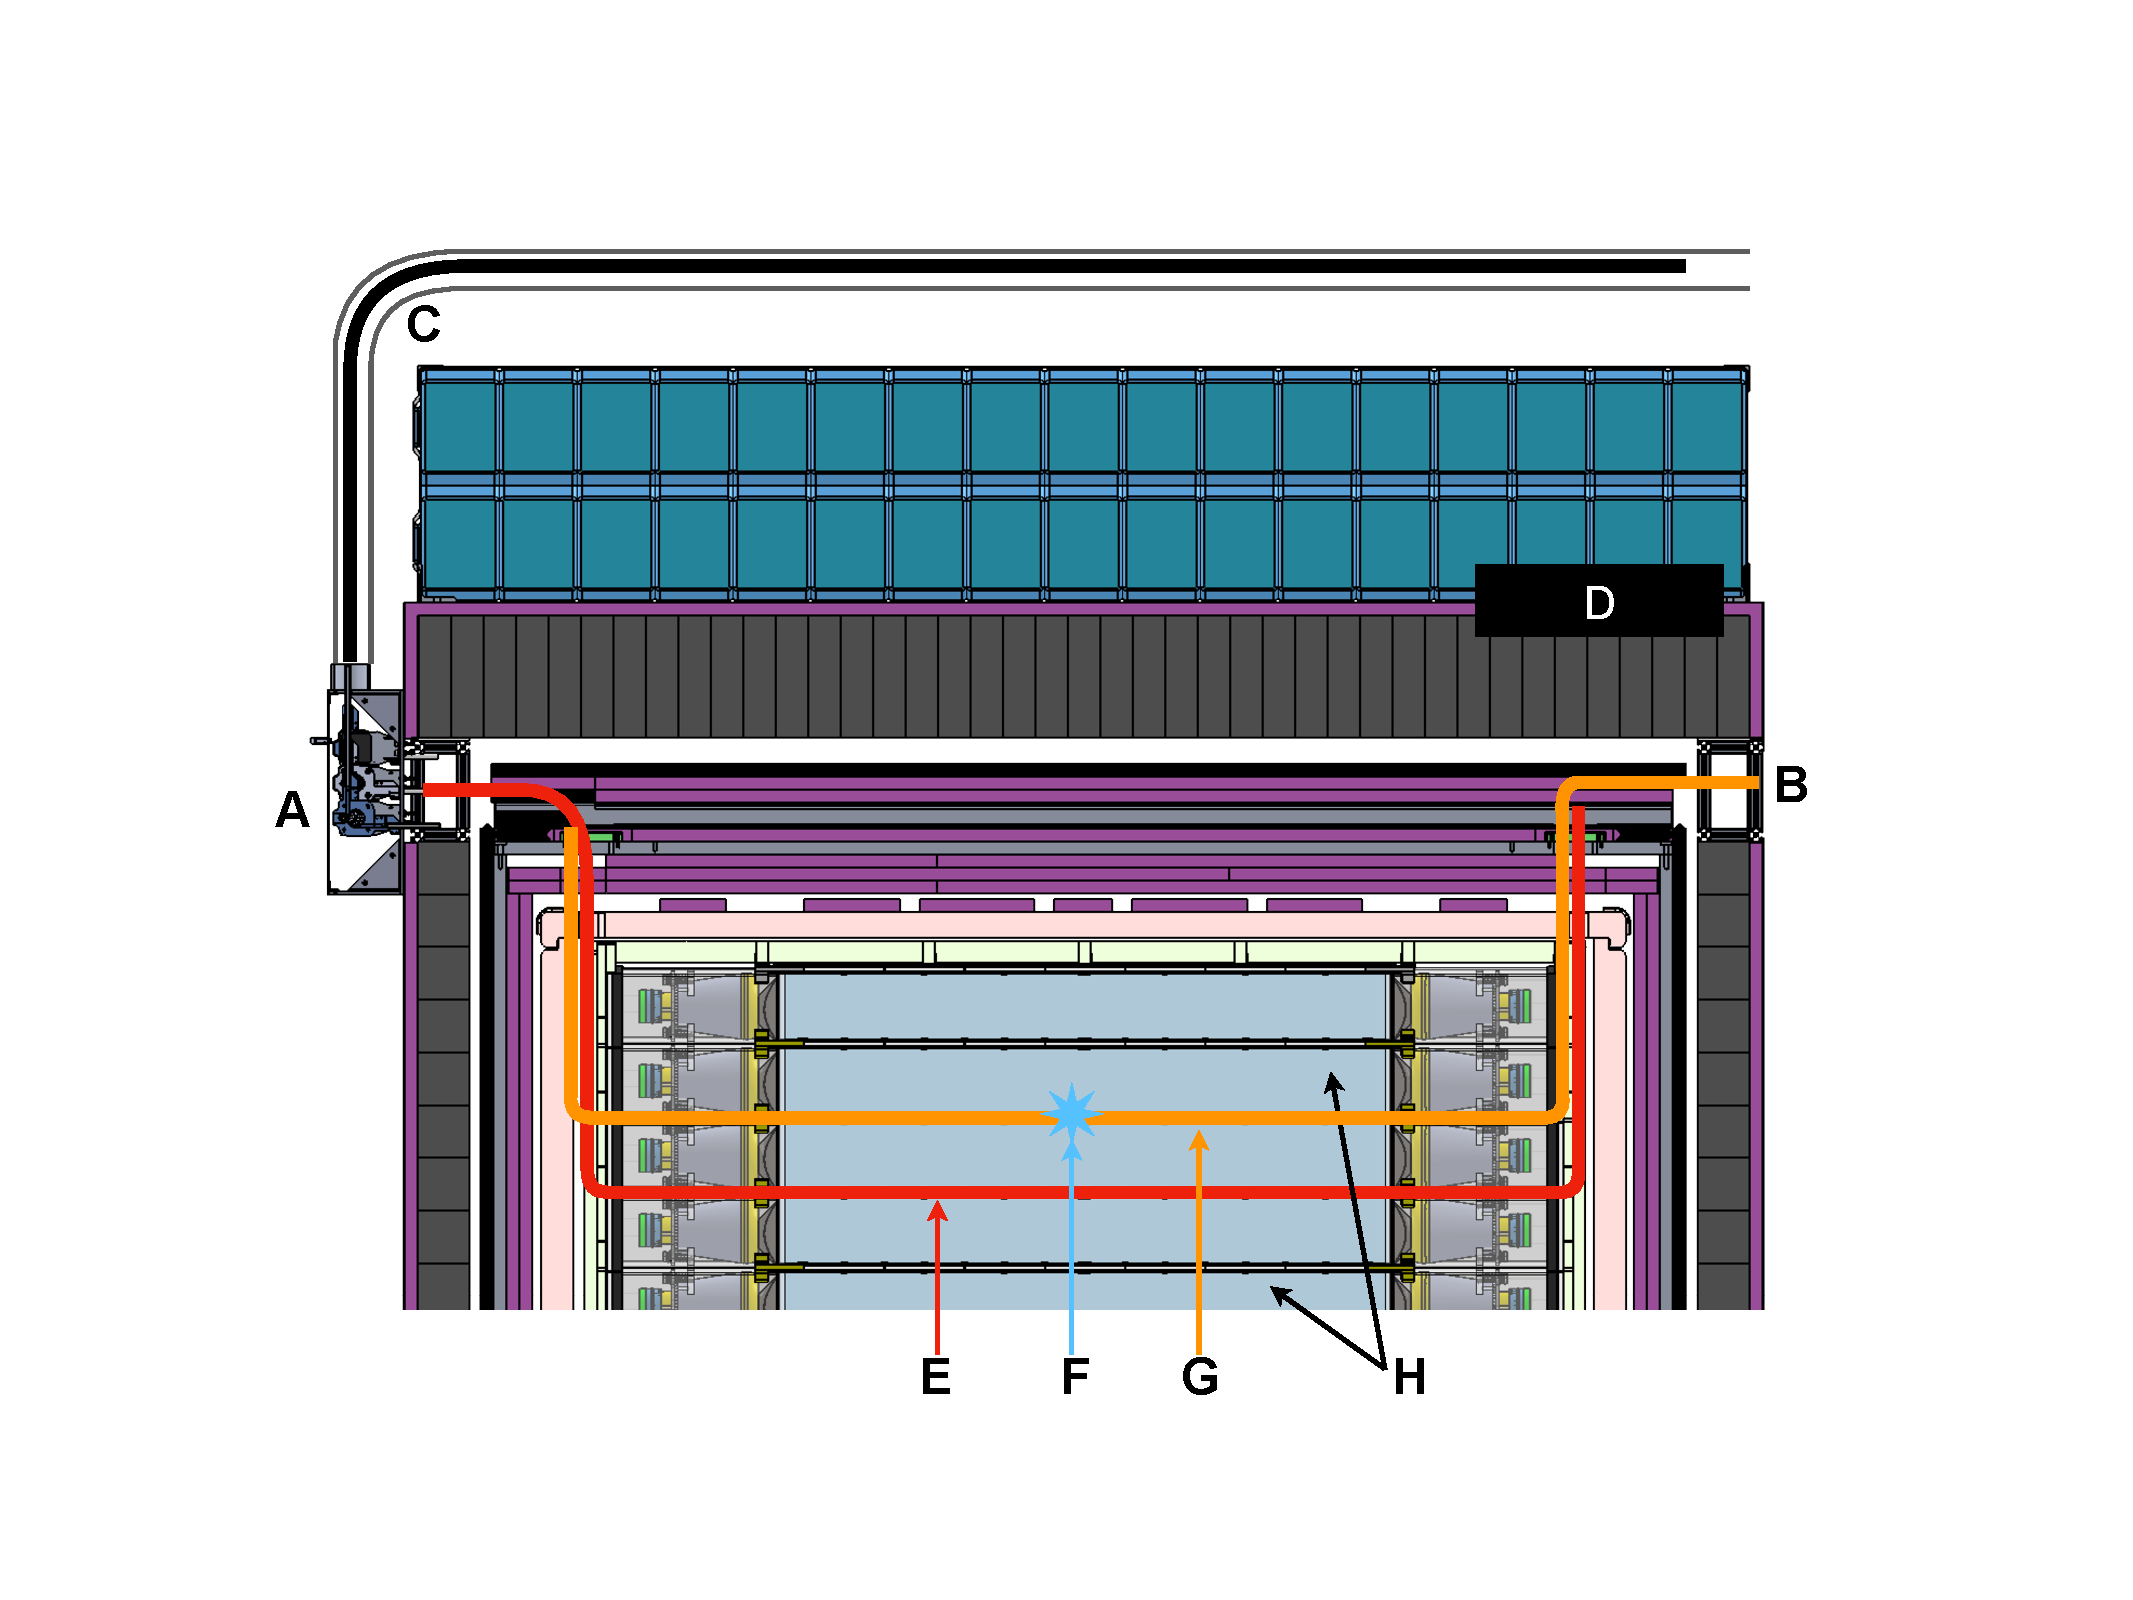
\includegraphics[width=0.7\textwidth]{Figures/CalibZ.pdf}
\caption[The setup of the PROSPECT calibration system]{
The setup of PROSPECT calibration system~\cite{bib:prospect_nim}.
(Top) Locations of OCS and radioactive source calibration tubes are shown on the (X, Y) plane. Yellow dots represent the OCS tube location, while red dots represent the radioactive source calibration location.
(Bottom) Detailed design of the calibration system along the axial direction (Z direction) of segments.
(A) source drive motors, (B) optical fiber connector panel, (C) belt storage tube,(D) shielding, (E) source deployment tube, (F) light injection point, (G) fiber tube, (H) detector segments. }
\label{fig:calibsystem}
\end{figure}

The goal of optical calibration is to characterize the single PE response of every segment by calculating the mean ratio of analog-digital converter (ADC) channel to count of PE. 
The OCS consists of a 15~mW single mode fiber-pigtailed laser diode assembled to a modified center PLA rod as a diffuse 450~nm wavelength light source.  
All 42 light sources deployed at the center of the selected PLA rods are connected to a high-performance laser generator. 

The radioactive calibration system inserts calibration sources into the detector to characterize detector response to physics events with known particle energy and vertex location.
Radioactive sources are sealed in cylindrical aluminum capsules with stainless steel caps to keep the radioactive sources sealed.
The capsules are attached to timing belts driven by motors installed outside of the shielded detector. 
To ensure smooth insertion of the calibration sources, polytetrafluoroethylene (PTFE) tubes are installed in the 35 PLA rods for calibration. 
The PTFE tubes also prevent direct contact between $^6$LiLS and the calibration system.
The dimensions of the capsules ($r = 3$~mm, $l = 12$~mm) are identical despite the differences in contained radioactive isotopes.
Because the capsule location is not visible in the detector, the calibration sources can be deployed precisely at the desired location by controlling the speed and time of source driving in the detector through 35 PLA rods as shown in Figure~\ref{fig:calibsystem}.

\Section{Detector Construction and Commissioning}
\label{sec:ad_construct}

The detector construction and commissioning consists of several phases: components fabrication, detector inner volume assembly, dry commissioning, detector shipment, $^6$LiLS filling, wet commissioning, external shielding assembly, and calibration source driver assembly.
The fabrication and assembly timeline is listed in Table~\ref{tab:timeline}.
During my thesis research, I also played major roles in the detector assembly, filling, wet commission, and initial calibrations.

\begin{table}[htpb]
\centering
\label{tab:timeline}
\caption[Detector assembly time line]{The fabrication and assembly timelines, as well as the primary locations of each mile stone.}
\begin{tabular}{cc}
\hline
Milestone & Date (Location) \\
\hline
Separator Delivery to Yale & 11/22/2016 (IIT) to 10/26/2017 (Yale) \\ 
PLA Delivery to Yale &  10/20/2016 (Autotiv) to 07/26/2017 (Yale) \\
PMT Module Delivery to Yale  & 1/2017 (Yale) to 11/10/2017 (Yale)\\
\hline
Detector Assembly & 10/30/2017 (Yale) to 11/17/2017 (Yale)\\
Detector Shipment  & 1/30/2018(Yale) to 1/31/2018 (ORNL) \\ 
$^6$LiLS Filling &2/24/2018 to 2/25/2018  (ORNL)\\
Wet Commissioning & 2/26/2018 to 3/17/2018 (ORNL) \\
External Shielding Assembly & 2/28/2018 to 3/3/2018 (ORNL)\\
Calibration System Assembly & 3/4/2018 to 3/5/2018 (ORNL)\\
\hline
\end{tabular}
\end{table}

The inner detector volume was assembled in a clean tent at Wright Laboratory, Yale University. 
The detector components, including optical grid components, PMT modules, and acrylic support, were assembled on a 6.3~cm thick transparent cast acrylic base, which is also the base of the liquid-tight acrylic tank. 
All components were subjected to thorough cleaning procedures: soaking and rinsing with 1\% Alconox solution (PLA rods were ultrasonic cleaned with the same solution) followed by Alconox removal with a 10~$\mathrm{M\Omega}$-cm water bath.
PMT modules were wholly filled with mineral oil to minimize bubbles appearing at the front windows.
The detector assembly was organized on a row-by-row basis.
The pre-assembled components (pre-strung PLA rods, separators, PMT housings, acrylic support plates, and other connection hardware) necessary for building a single horizontal row of 14 PROSPECT segments were transported into the detector assembly cleanroom during one shift. 
At the beginning of each shift, final combinations of one separator and one strung PLA rod were pre-assembled together for ease of assembly.
Procedures of assembly are briefly overviewed in Figure~\ref{fig:assemble_procedure}.
Photographs of the detector assembly, in Figure~\ref{fig:ADAssemble}, indicate the details of the component interlocking.

\begin{figure}[h!]
\centering
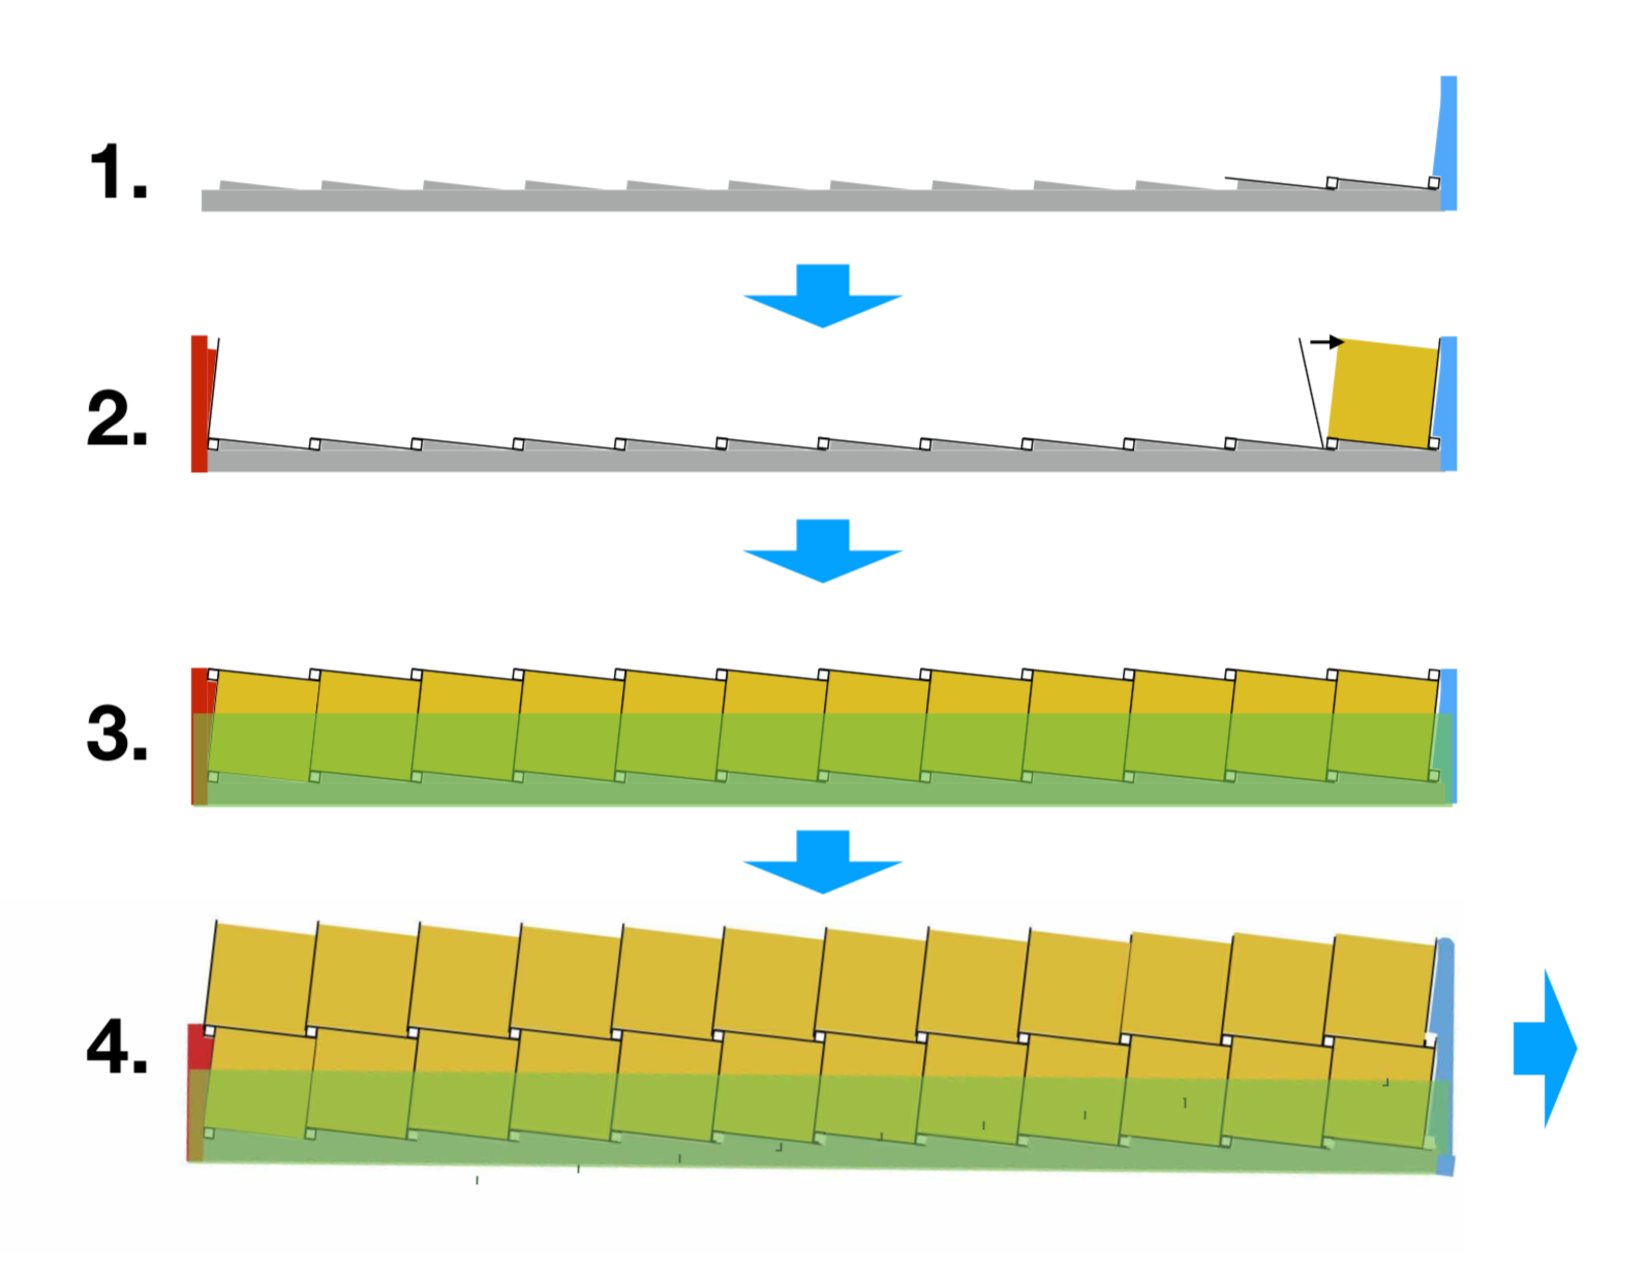
\includegraphics[width=0.48\textwidth]{Figures/OGAssemble1.pdf}
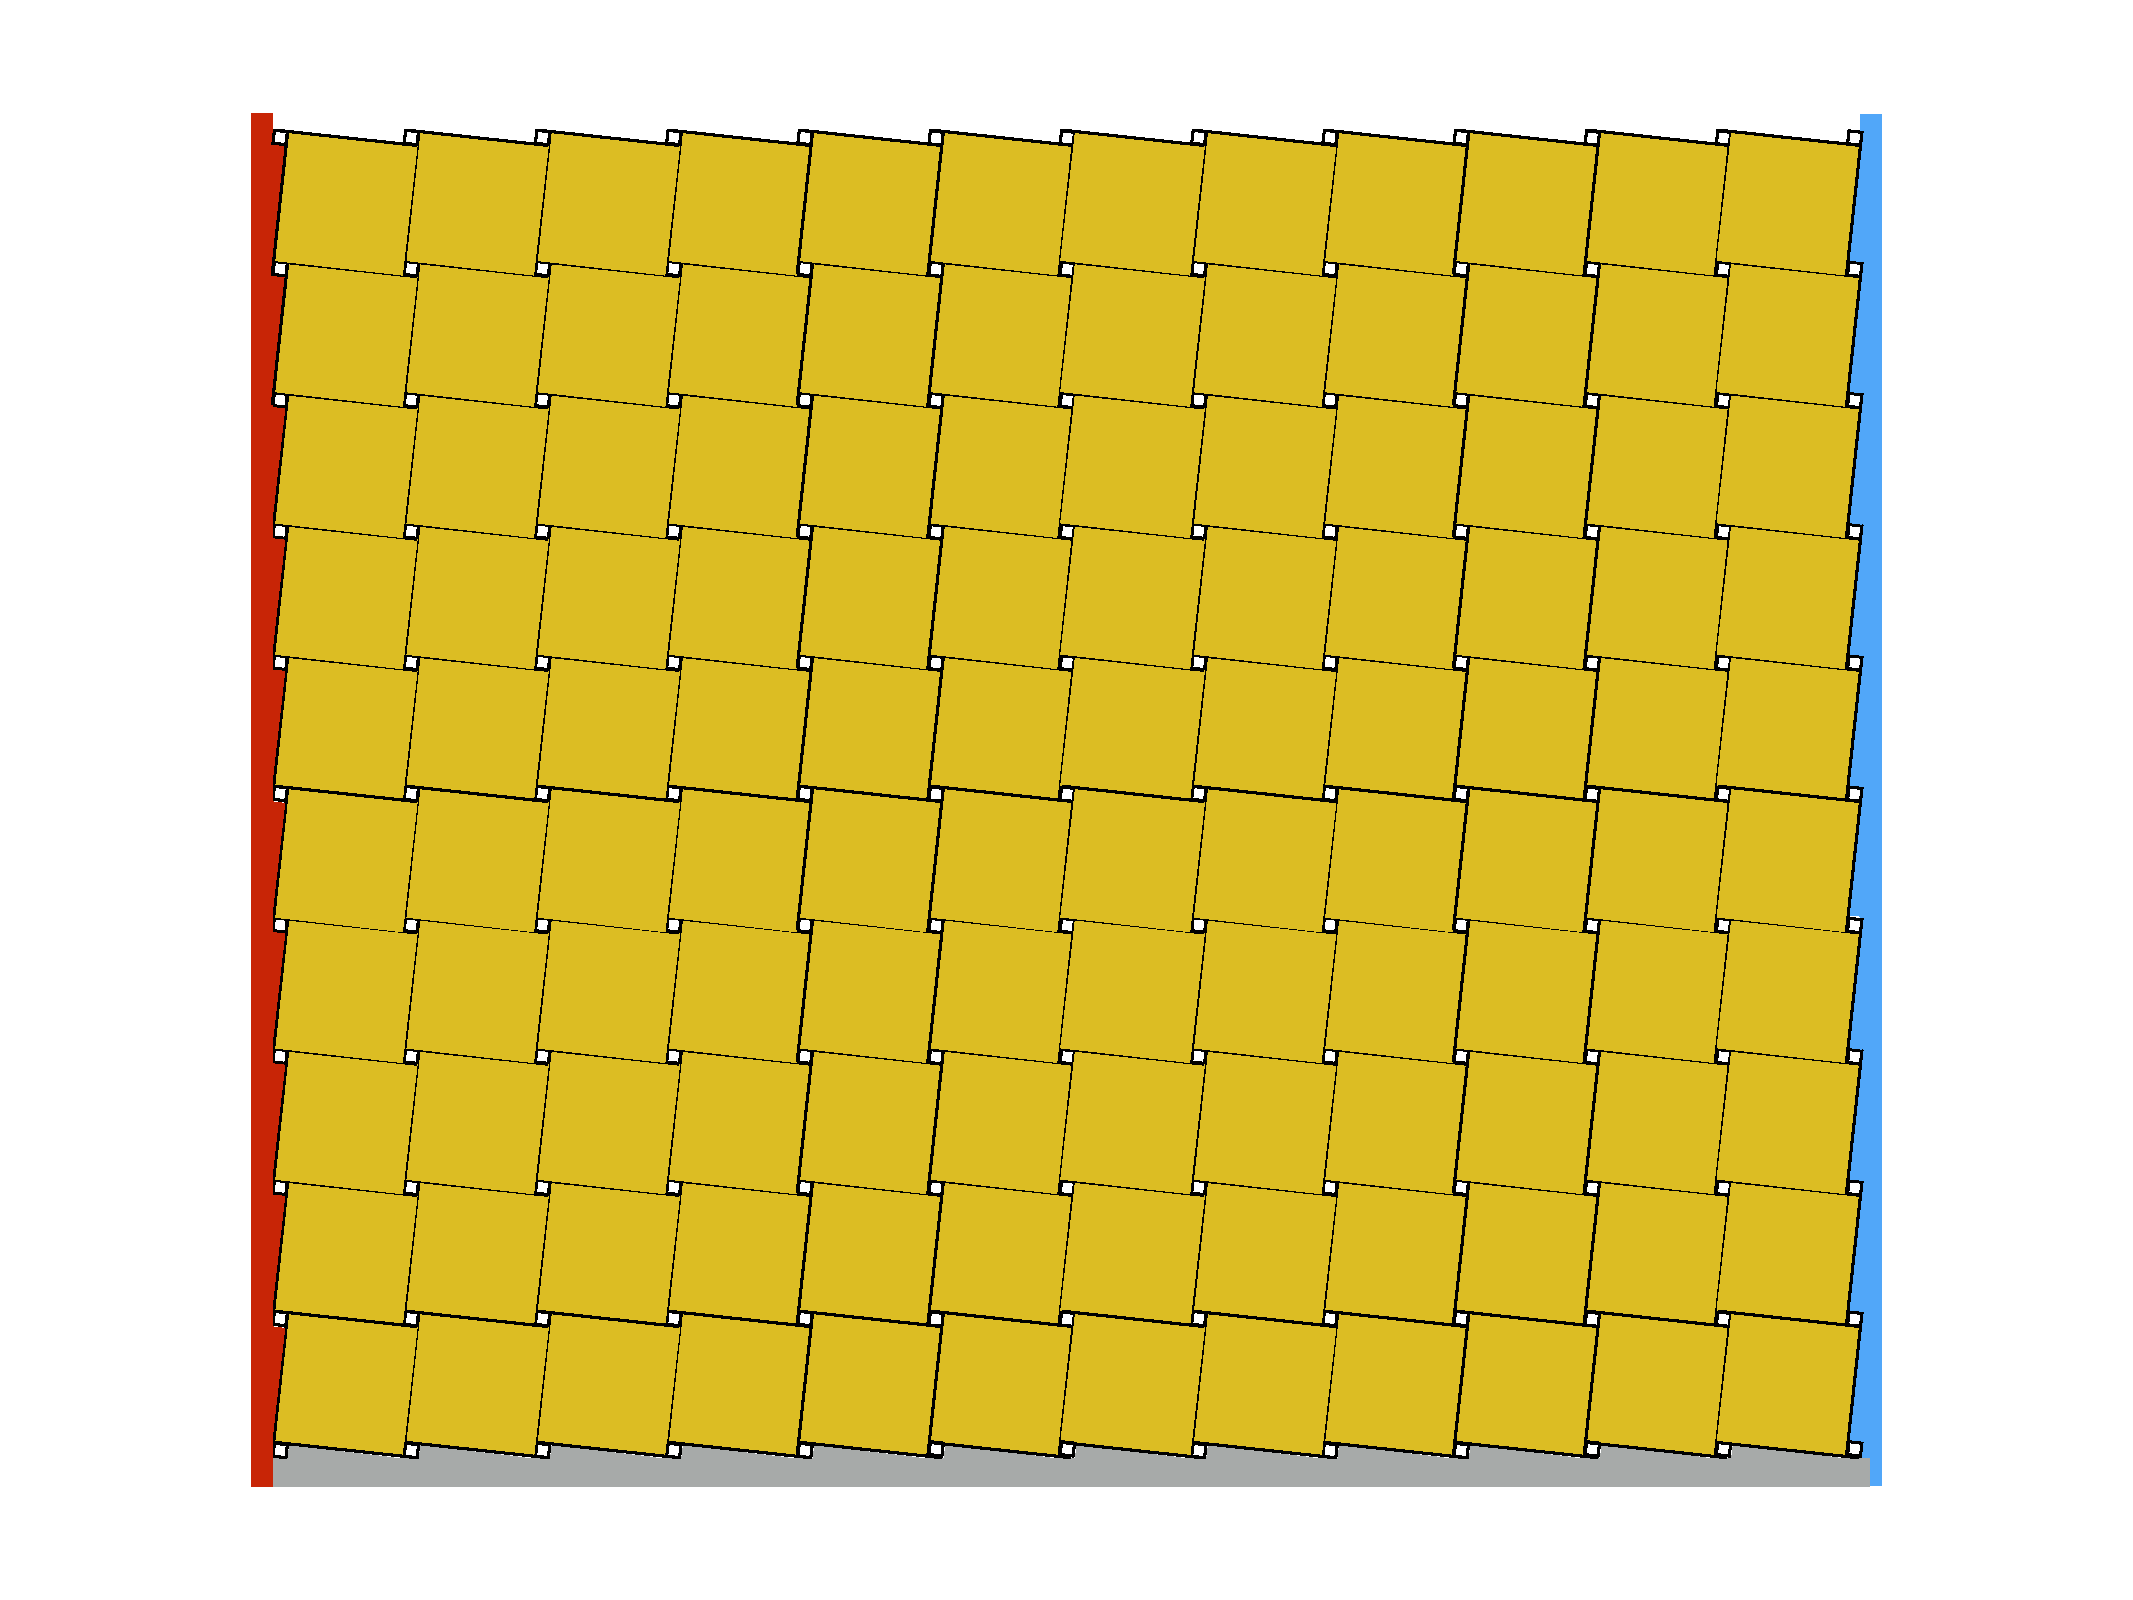
\includegraphics[width=0.48\textwidth]{Figures/OGAssemble2.pdf}
\caption[Optical grid assembly illustration]{Illustration of the optical grid assembly procedure~\cite{bib:prospect_og}, where the black lines represent separators, the white squares represent PLA rods, the yellow squares represent PMT housings, and other colored parts are acrylic support plates.
(1) The first-layer horizontal separators and PLA rods being assembled upon the base acrylic support plates.
(2) The first-layer vertical separators assembled with PMT modules.
(3) The second-layer horizontal separators and PLA rods assembled upon the first layer, closing the bottom row segments, with the green shade representing end acrylic support plates that constrained the PMT housing positions.
(4) The following rows of segments were assembled similarly until the optical grid subsystem was assembled.
}
\label{fig:assemble_procedure}
\end{figure}

\begin{figure}[h!]
\centering
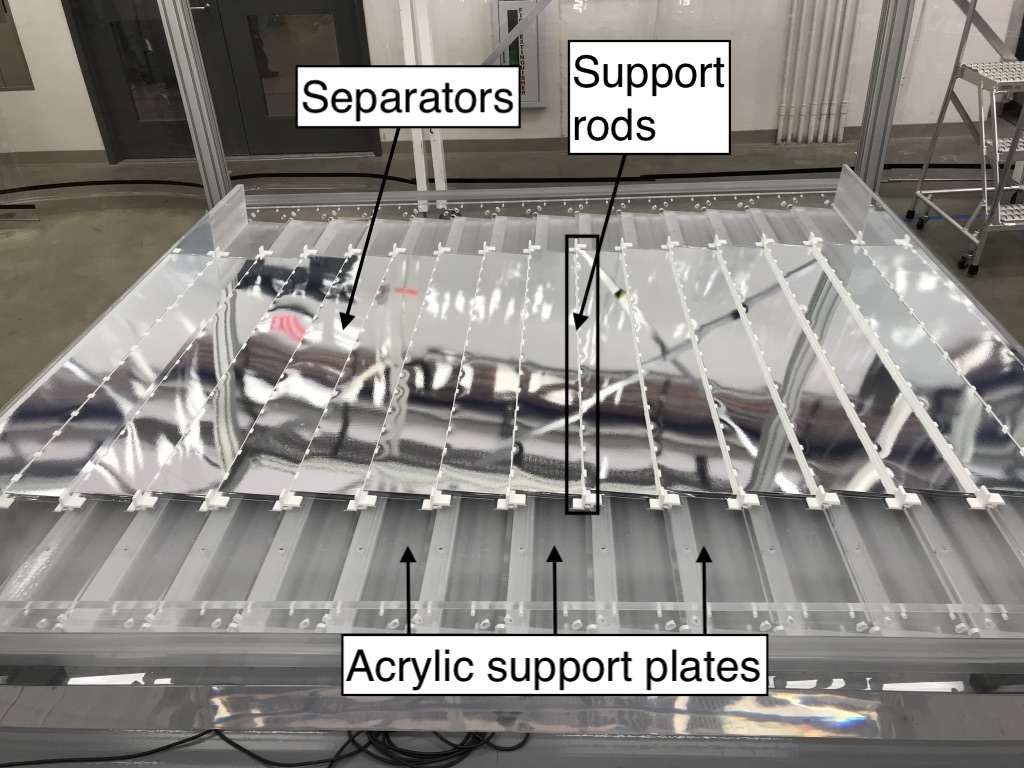
\includegraphics[width=0.45\textwidth]{Figures/Firstlayer.jpg}\quad
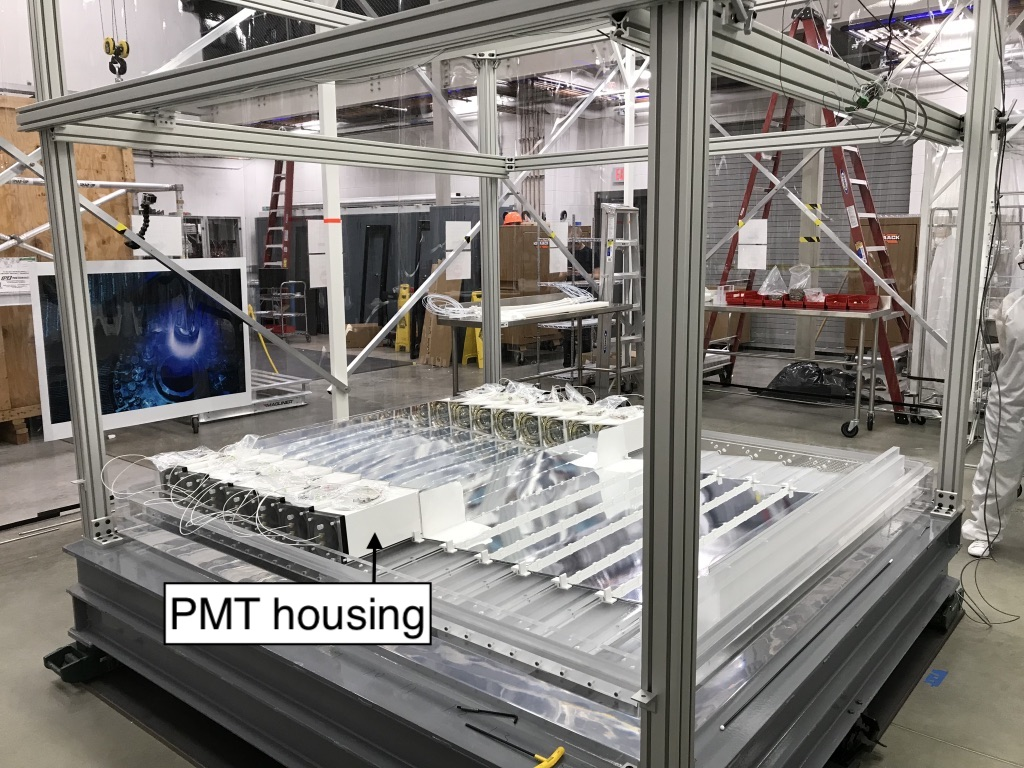
\includegraphics[width=0.45\textwidth]{Figures/OngoingAssembly.jpg}\\
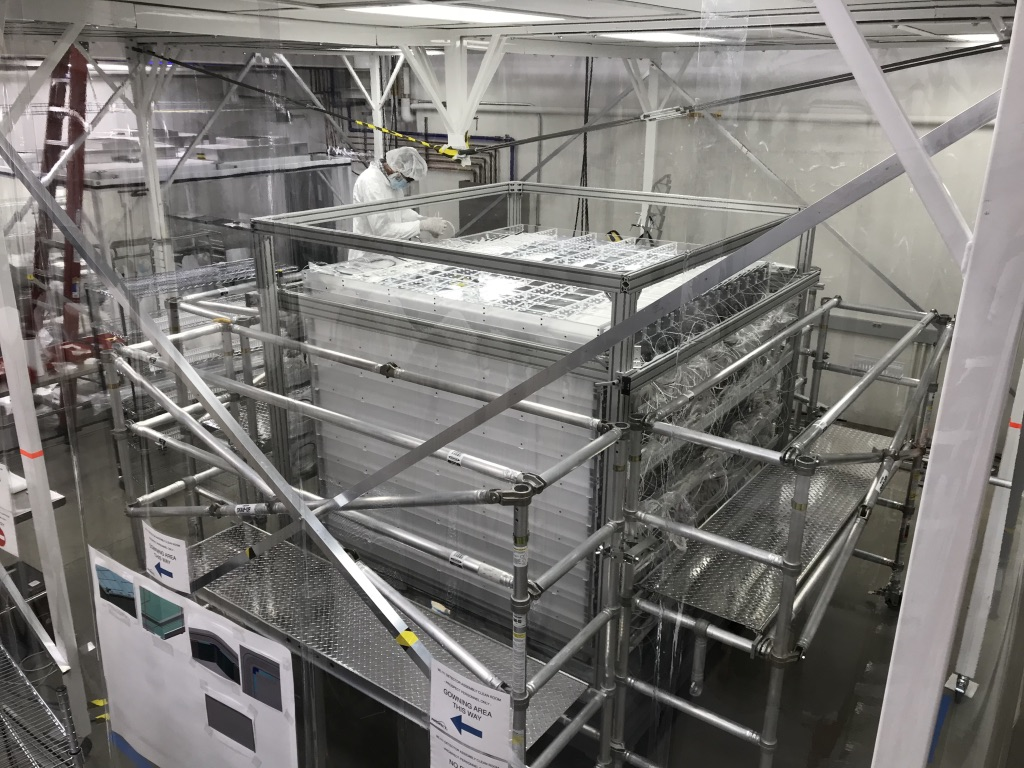
\includegraphics[width=0.45\textwidth]{Figures/FinishedAssembly.jpg}
\caption[The photograph of the PROSPECT AD assembly]{
(Top left) The bottom layer of the assembled PLA rods and separators on the acrylic support plates.
(Top right) The assembly of the bottom layer with PMT modules stacking on the acrylic support plates. 
(Bottom) Photograph of the assembled inner detector.}
\label{fig:ADAssemble}
\end{figure}

To ensure dimensional uniformity, a precise metrological survey was conducted after the assembly of every row with a custom-made aluminum gauge and laser height measurement system.
This survey was conducted to measure the horizontal and vertical difference among assembled separators and PMT modules.
The goal of the metrological survey is to constrain the segment volume variation within 1\%.
Additional $\sim$0.25~mm FEP shims were placed between PLA rod end spacers and PMT housing bodies in the next-row assembly as needed.  
Shim placements and thicknesses were dictated by the results of the metrological survey of the previous row.  
The calibration source guiding tubes were inserted into the desired PLA rods as the acrylic rods used to string the PLA rods were removed.
Several temperature sensors were also inserted into specific PLA rods.

The assembled detector was contained a transparent acrylic tank with 6.3~cm thick walls, whose inner dimension is  1.995~m (wide) $\times$ 2.143~m (long) $\times$ 1.555 m (tall).
The acrylic walls and base were combined with Viton o-rings to ensure a liquid tight condition.
The lid of the acrylic tank allows the feeding of PMT signal and HV cables through. 
Environmental sensors, including liquid level sensors, oxygen level sensors, and nitrogen cover system, were also installed through this lid.
After the detector was securely contained in the acrylic tank, the acrylic tank was moved into an aluminum tank.
The dimensions of the aluminum tank are 2.255~m (wide) $\times$ 2.205~m (long) $\times$ 1.982~m (tall).
The goal of the aluminum tank is to provide a light-tight condition of the PROSPECT AD and additional protection during detector shipment. 
Borated polyethylene boards with various thickness were filled between the acrylic tank and the aluminum tank, uniformly surrounding the former.
A photograph of the acrylic tank and the aluminum tank is shown in Figure~\ref{fig:tanks}

\begin{figure}[h!]
\centering
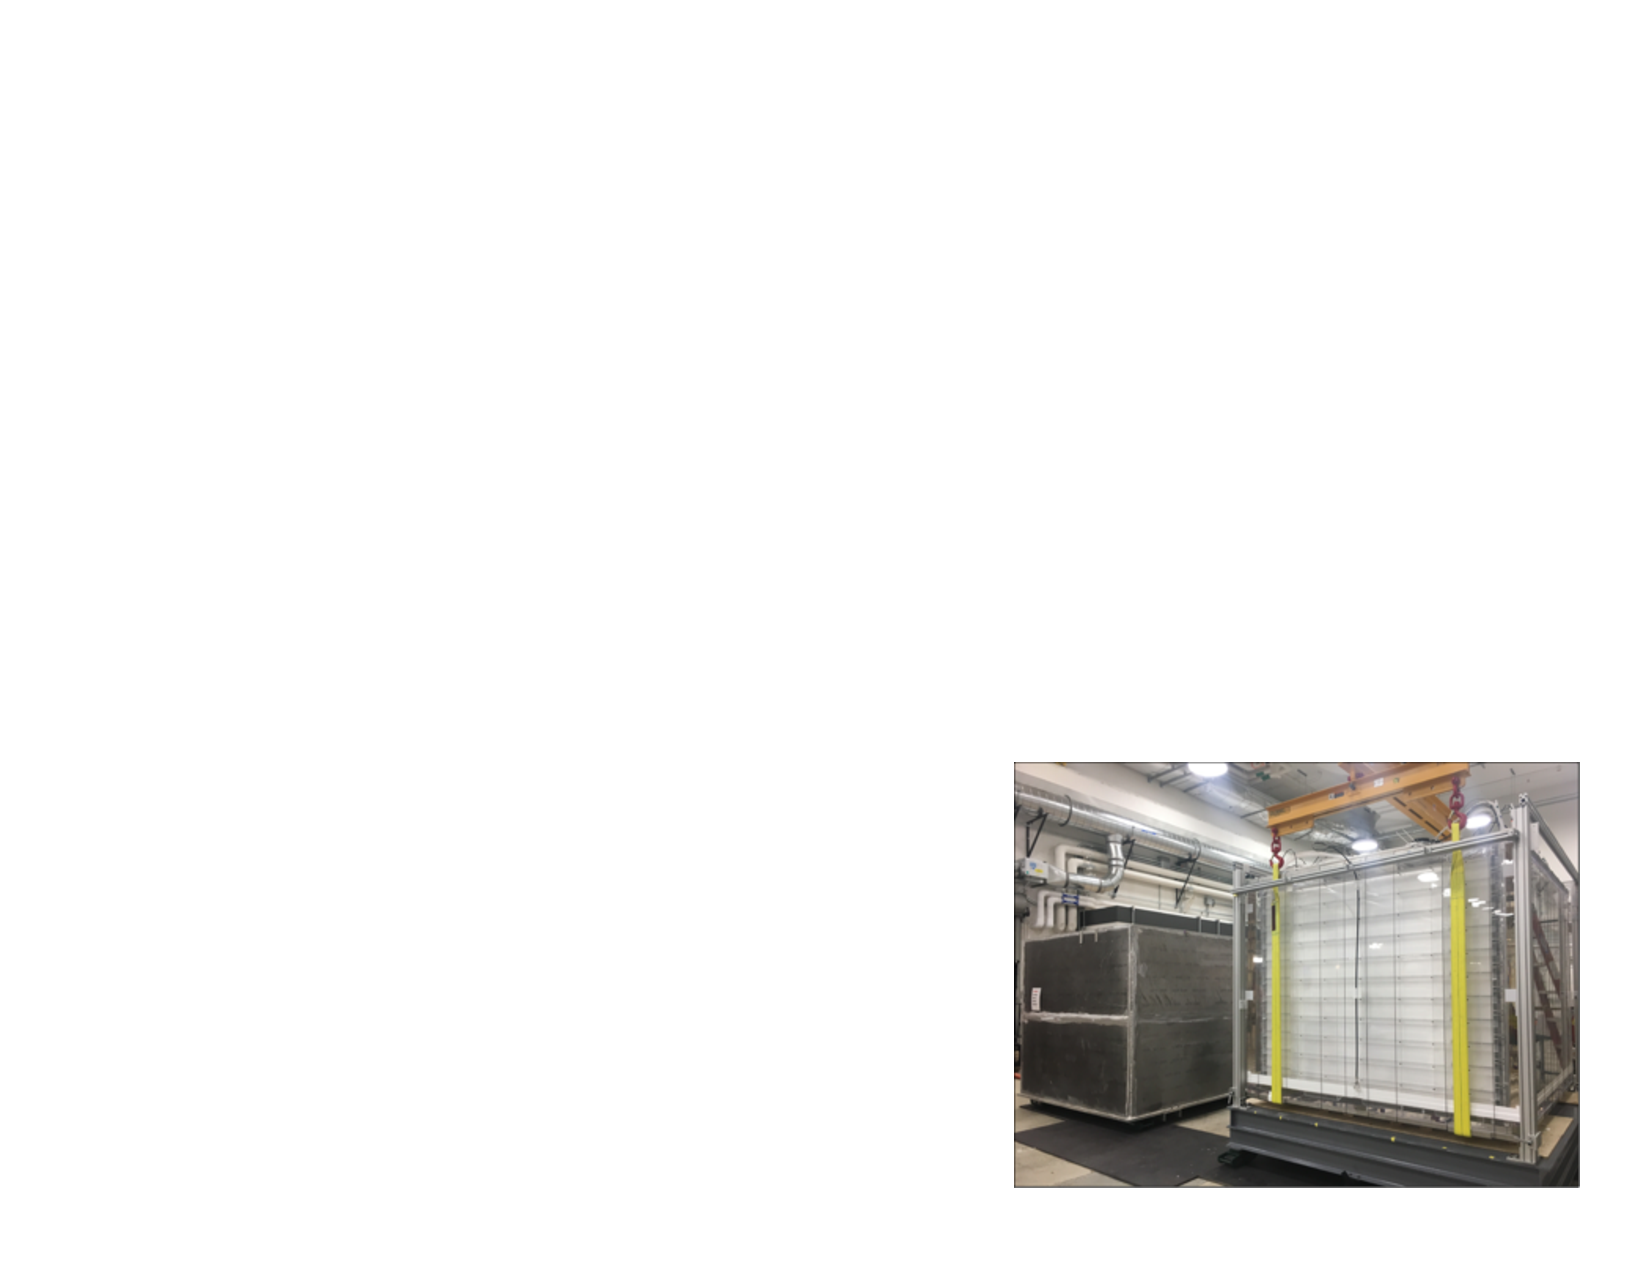
\includegraphics[width=0.6\textwidth]{Figures/Tank.pdf}\quad
\caption[The acrylic and aluminum tanks as containment vessel of the detector]{
The aluminum (left) and acrylic (right) tanks as containment vessel of the PROSPECT inner detector volume.}
\label{fig:tanks}
\end{figure}

The assembled PROSPECT AD was tested with an unfilled detector (dry commissioning) at Yale University, demonstrating the electronic performance and the data acquisition (DAQ) system via collecting the OCS data and cosmic ray background data.
After the dry detector test, the PROSPECT AD was shipped from Yale University to the HFIR building. 
The detector was cushioned by 0.1~m thick foam underneath and 0.05~m thick foam surrounding, in a wooden shipment crate.
A 3$\times$3 detector mock-up was tested to simulate the vibration and shock during detector shipment.
No damage was observed in the shipment simulation.
 
The $^6$LiLS were shipped in drums to ORNL with nitrogen cover gas.
The temperature was controlled during the $^6$LiLS shipment.
Before the detector filling, all $^6$LiLS was pumped into a 20-ton Teflon lined shipping container (ISO tank). 
Nitrogen was used as cover gas for both the detector and the ISO tank during the $^6$LiLS filling.
The detector is tilted $0.7^\circ$ along the axial direction of the segments to avoid bubbles being retained in the segments.
The filling rate of the $^6$LiLS was set to 3~liter/minute with an ultrasonic sensor monitoring the liquid level.
There were 4340~kg $^6$LiLS filled into the detector acrylic tank.

The external shielding includes a local shielding wall and detector passive shielding. 
The local lead shielding of a 0.1~m thickness was installed between the wall of the reactor pool and the detector.
The detector's passive shielding appears in several layers surrounding the detector.
From inside to outside, the passive shielding consists of a layer of 2.5~cm thick borated polyethylene, a layer of 2.5~cm thick layer of lead for gamma shielding, and a layer of 2.5~cm to 7.5~cm thick high-density polyethylene as a neutron absorber. 
On top of the detector, a layer of 0.46~m tall water bricks was added as additional overburden to suppress cosmogenic neutron background.

The radioactive source driving motors and the nitrogen flow control system were installed outside of the shielded detector. 
The HV cables and signal cables were connected to a DAQ crate for full detector commissioning.
A photograph of the installed detector is shown in Figure~\ref{fig:finish}.

\begin{figure}[h!]
\centering
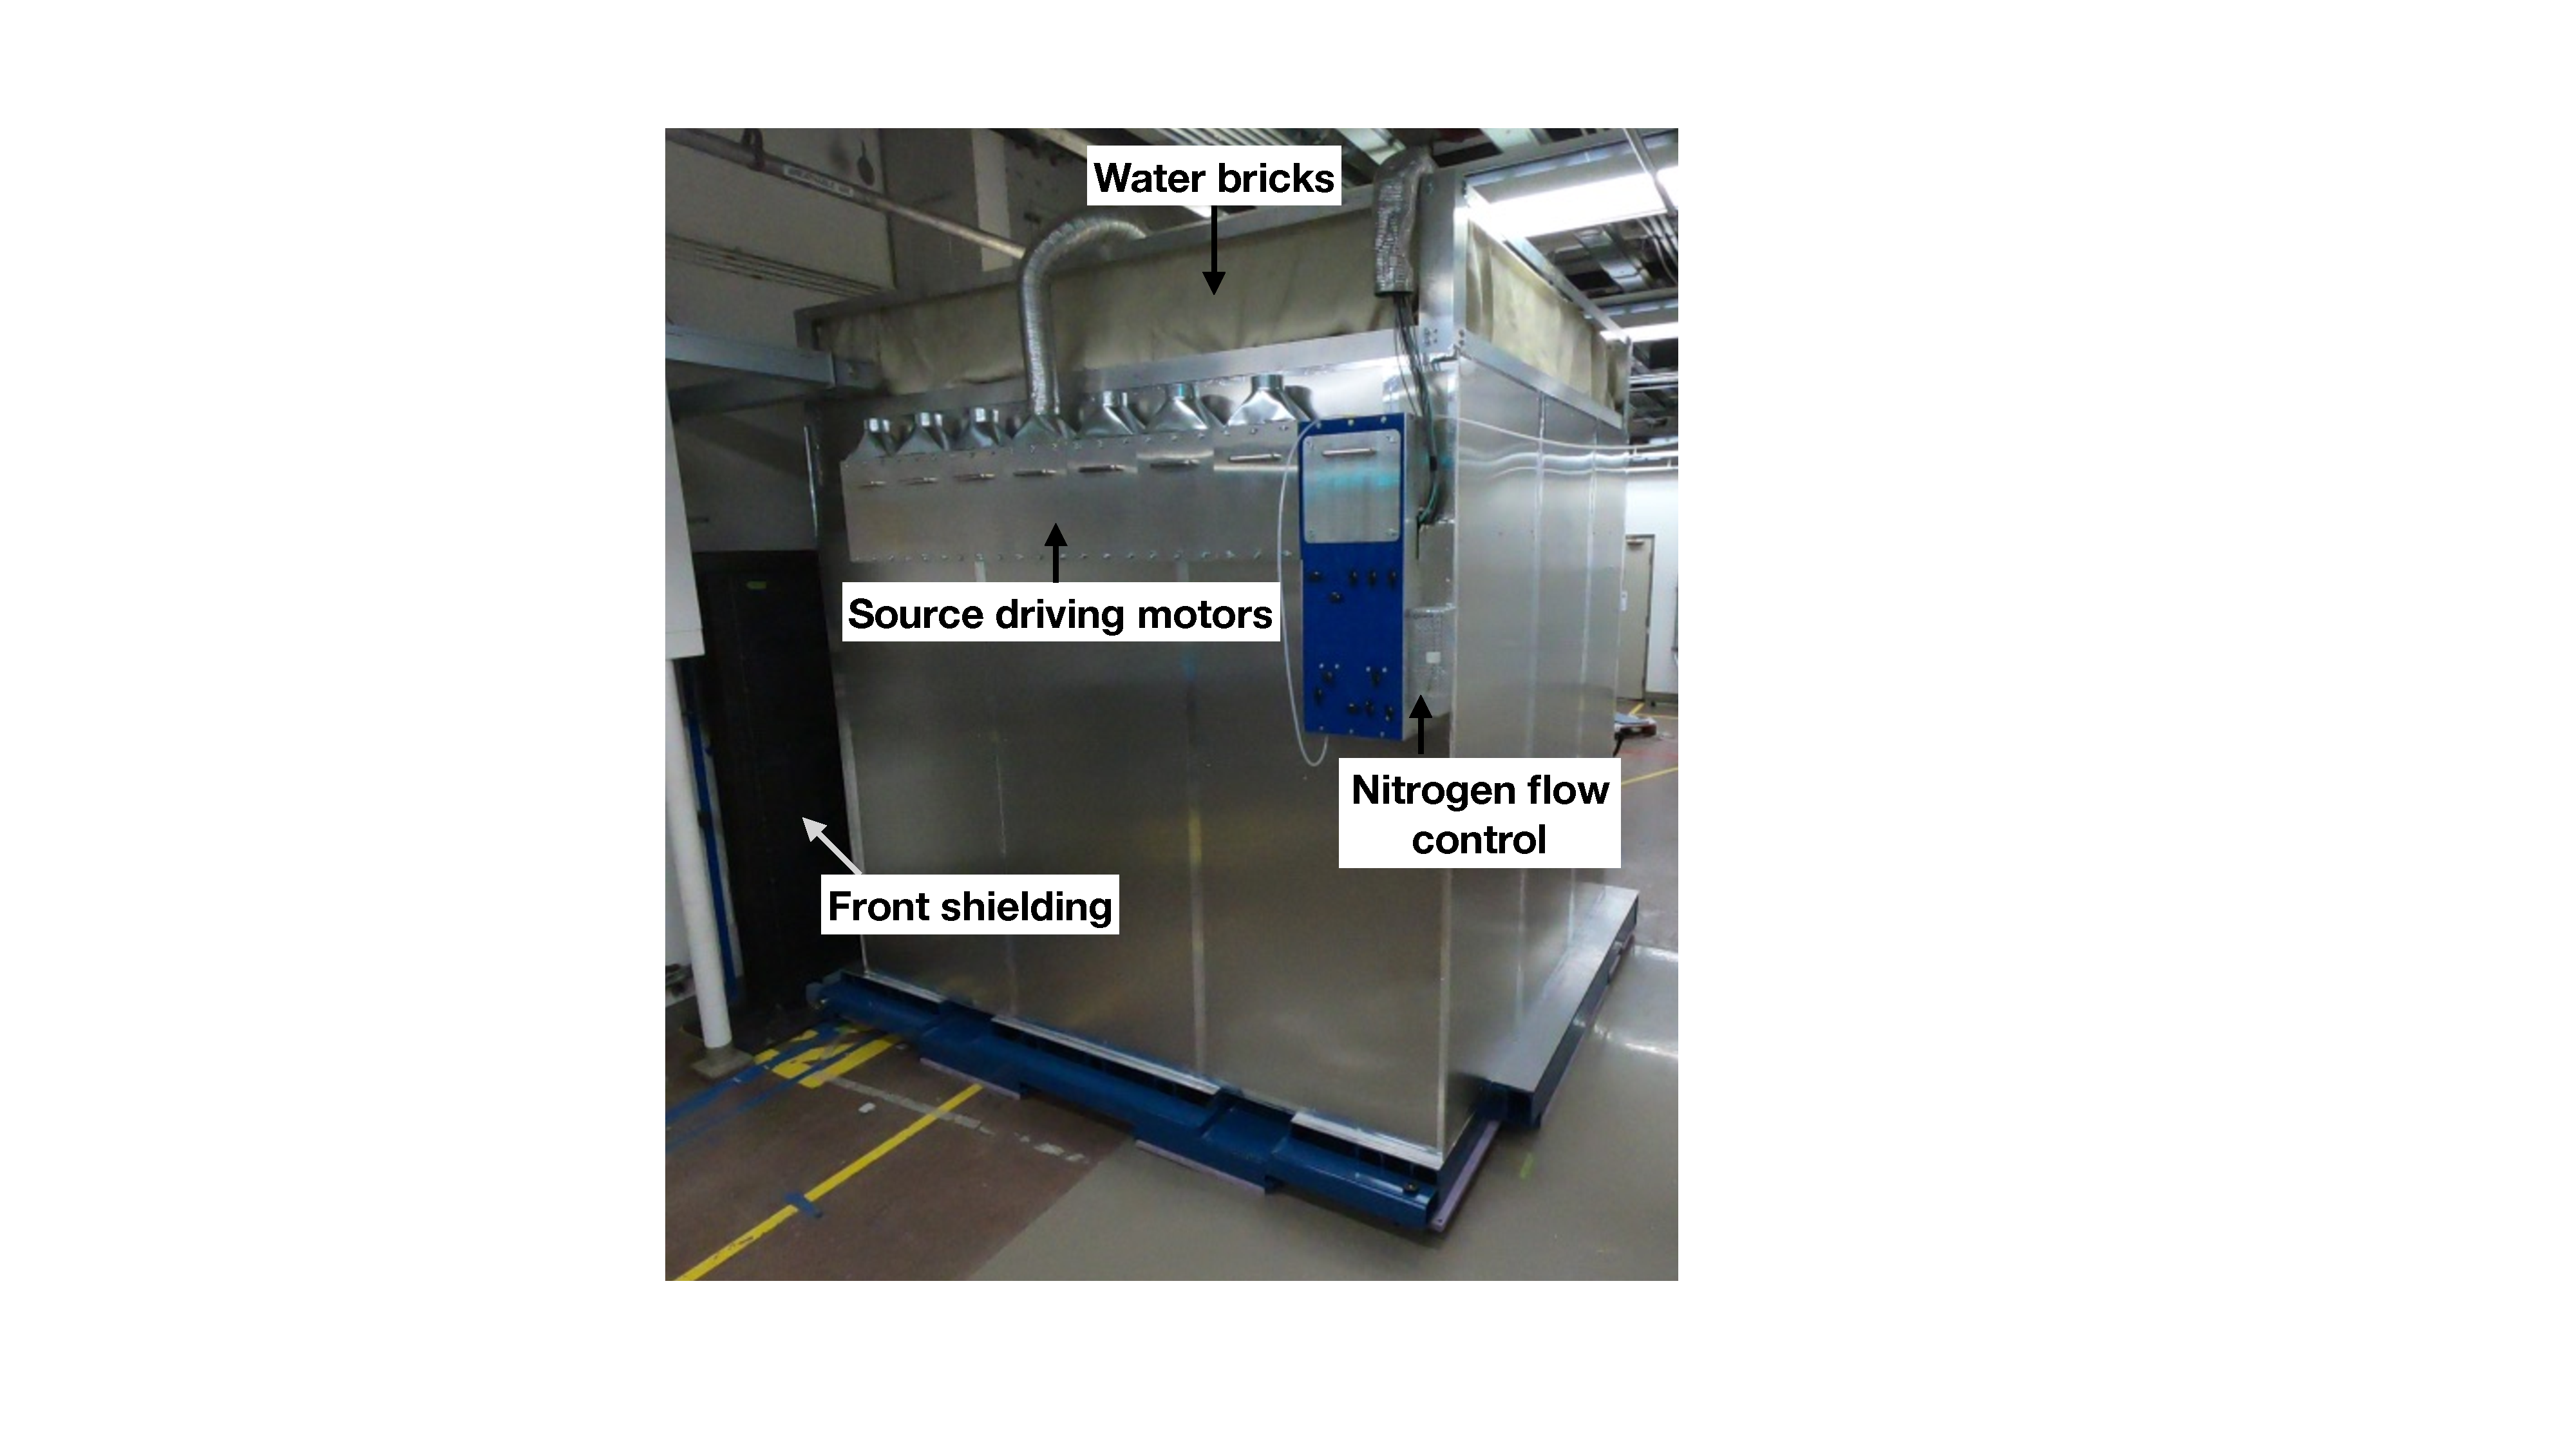
\includegraphics[width=0.6\textwidth]{Figures/AssembledDetector.pdf}\quad
\caption[The installed PROSPECT AD]{
A photograph of the PROSPECT AD. 
The calibration source motors and nitrogen flow control systems were shown on the side of the detector.}
\label{fig:finish}
\end{figure}

\Section{Data Acquisition System}

The DAQ system, shown in Figure~\ref{fig:DAQ}, is composed of 21 CAEN V1725 16-channel digitizers (ADC) with 250~MHz sampling rate, a Phillips Scientific 757D NIM Fan-In/Fan-Out module, two DAQ control systems, a local storage array, and a run control computer.
Each channel of the digitizers is connected to one of the 308 PMT signal output cables.
The ADCs are grouped into two, operated by two VME crates, and controlled by two computers.

\begin{figure}[h!]
\centering
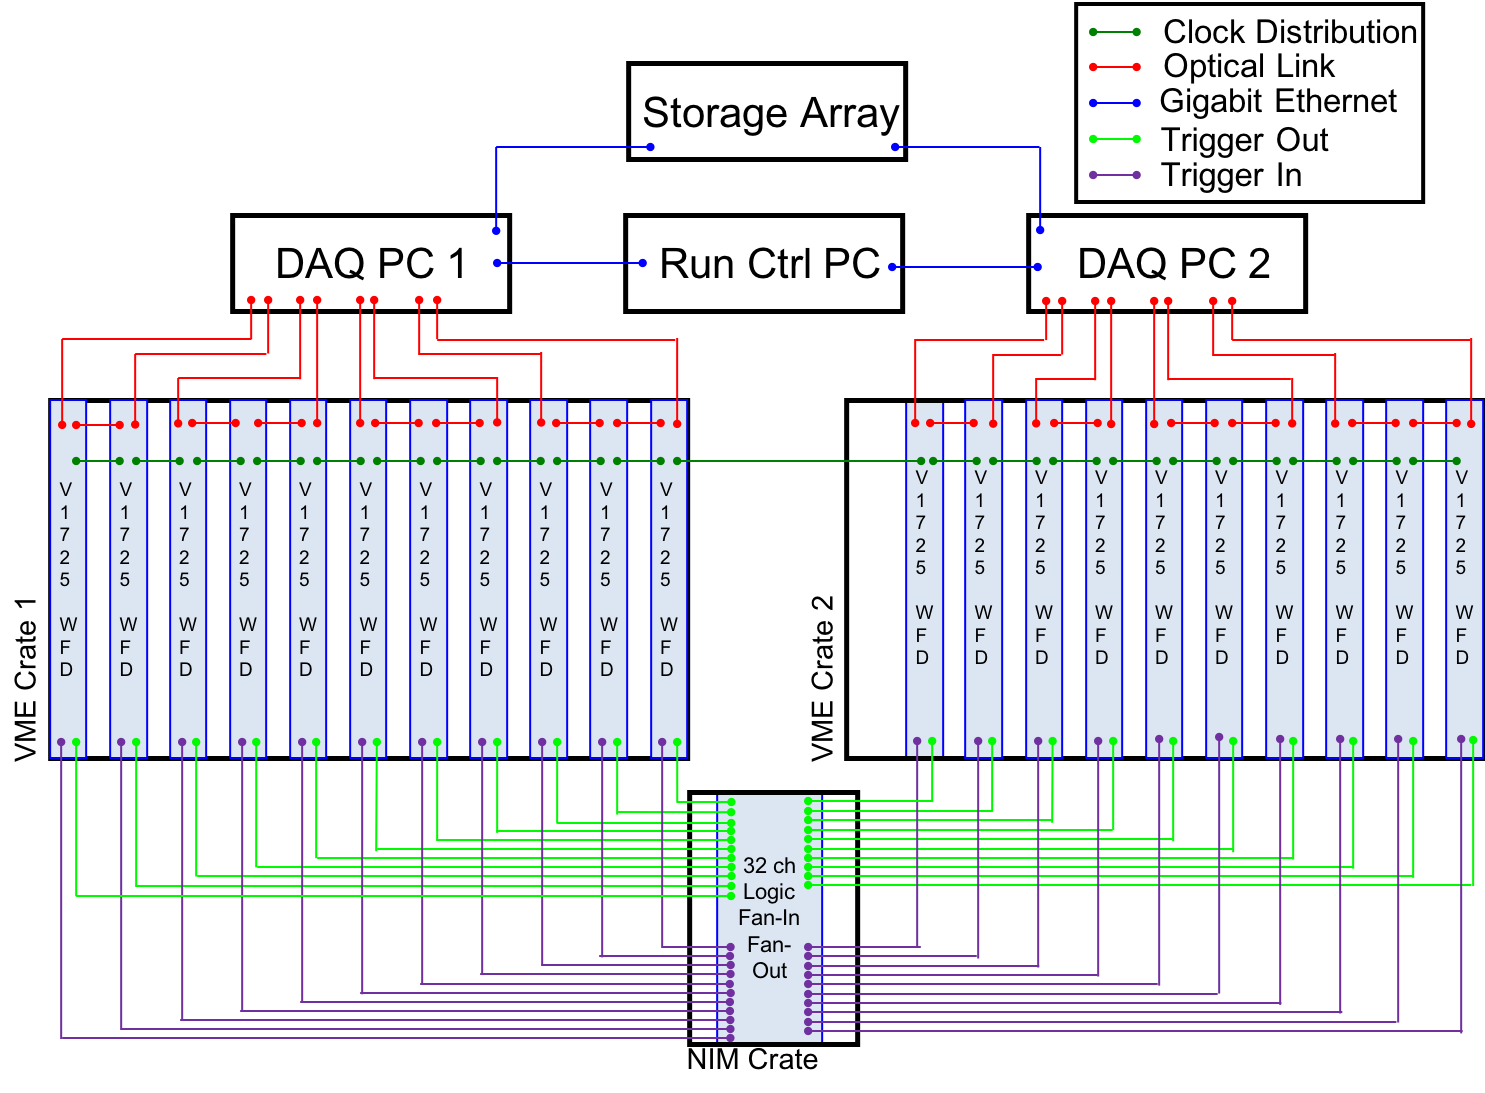
\includegraphics[width=0.95\textwidth]{Figures/DAQ.png}\quad
\caption[DAQ system connection]{
Schematic diagram of the DAQ system.}
\label{fig:DAQ}
\end{figure}

The dynamic range of the data collection is set by adjusting the HV gain of the PMT channels.
In order to exclude cosmic ray background and cover the range of IBD prompt energy, as well as the cosmogenically produced $^{12}$B beta energy spectrum, the dynamic range of the general data acquisition is set to 15~MeV.
During optical calibration, the dynamic range is narrowed down by increasing the gain to cover the single PE regime.
The acquisition window of an ADC pulse is 148 samples long, equivalent to 592~ns. 
The DAQ triggering logic is shown in Figure~\ref{fig:trigger}.
The DAQ system is triggered on thresholds of the ADC signal height collected from each PMT.
A 50~channel primary trigger threshold, which is equivalent to the signal magnitude of approximately five PEs, is set (later changed to 25~channel considering light yield decrease) to trigger the DAQ logic. 
When the pulse heights from both PMTs of one segment exceeds the primary threshold within a 64~ns coincidence window, a zero length encoding (ZLE) threshold is set to trigger the light collection of each PMT.
The pulses from all PMTs whose height exceeds the 20~channel ZLE threshold, are recorded to the local storage.
These thresholds were set to balance the PROSPECT AD's ability to reconstruct the 511~keV positron-electron annihilation gamma-ray and the size of lower energy datasets.

\begin{figure}[h!]
\centering
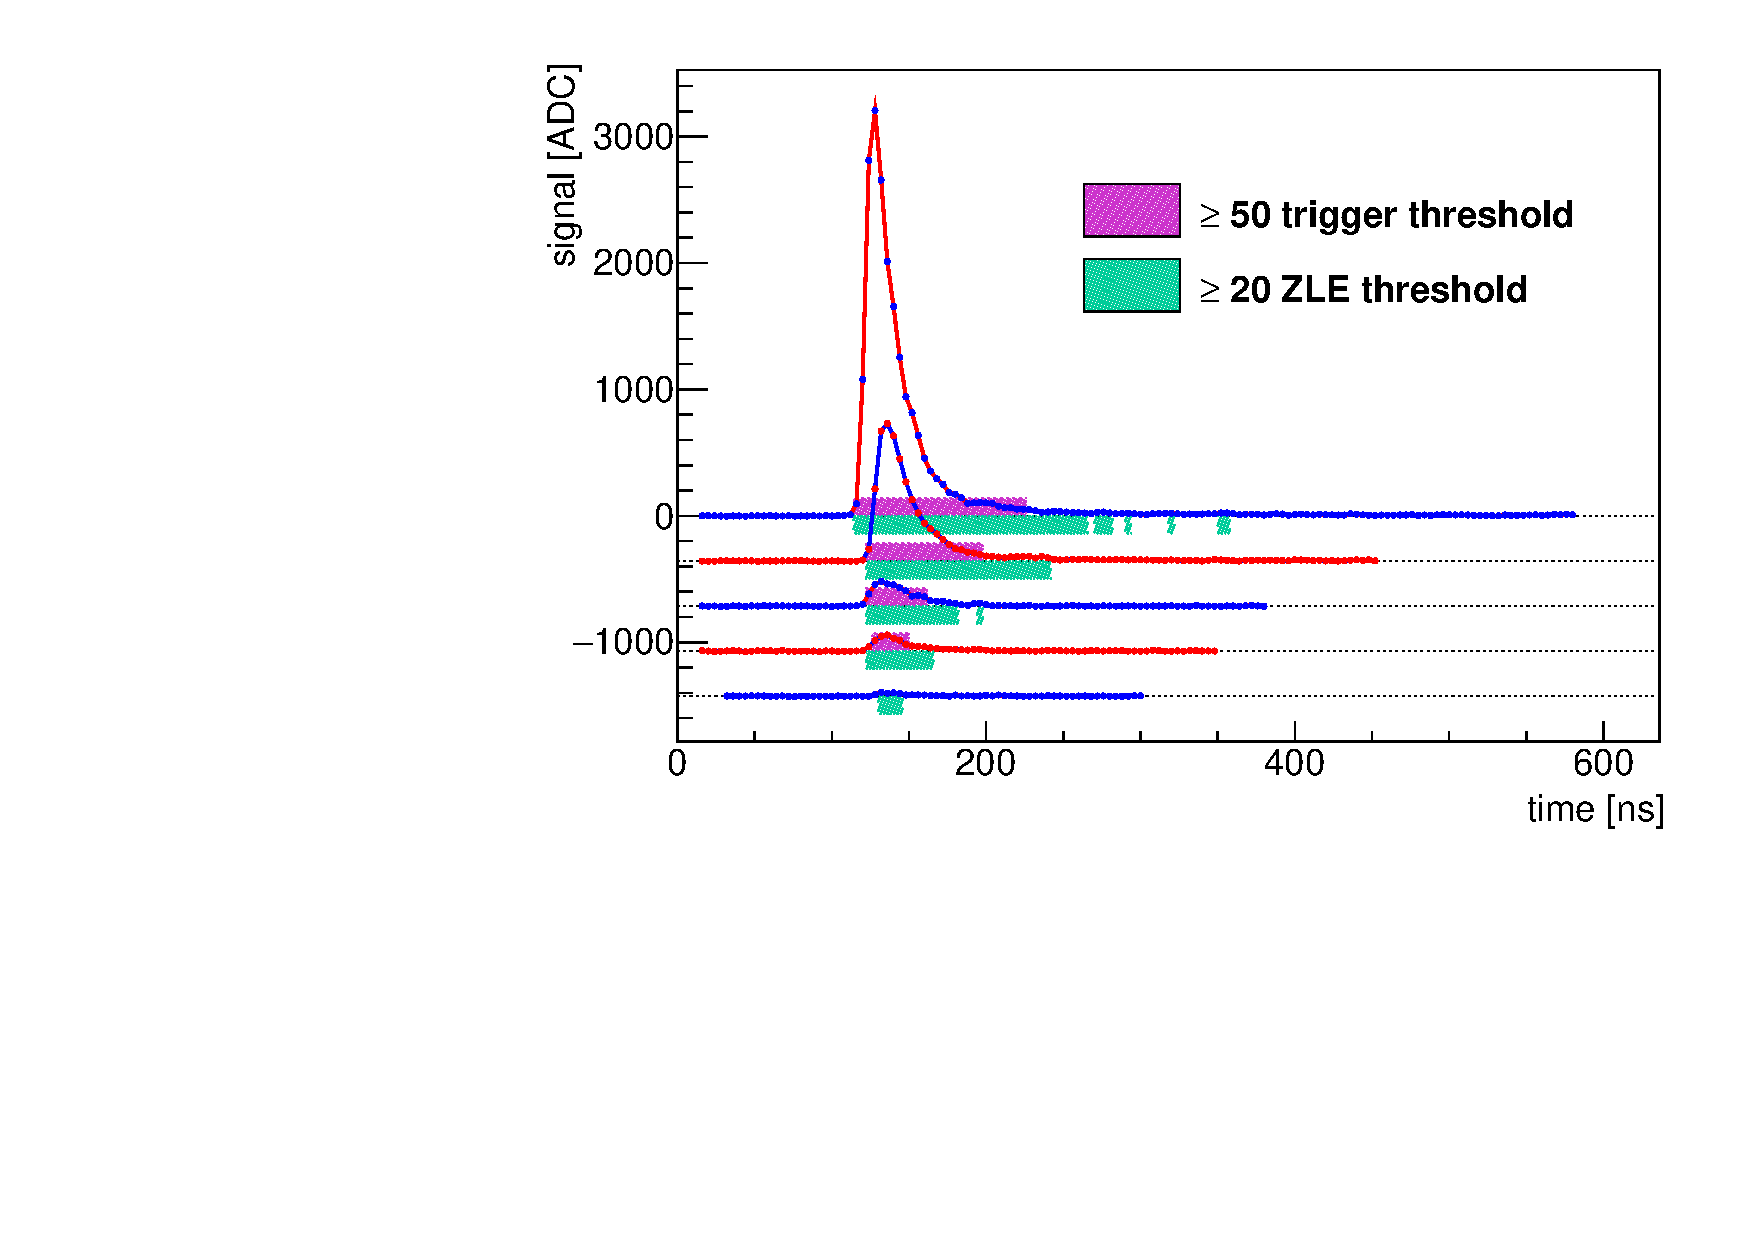
\includegraphics[width=0.95\textwidth]{Figures/Triggering.pdf}\quad
\caption[DAQ triggering signal]{
Example of a DAQ triggering signal, where the pulses are collected from different PMT channels.
The DAQ trigger is generated by the coincidence of the highest pair of a pulse from a single segment.
The following pulses with a height exceeding the ZLE threshold are saved in data.}
\label{fig:trigger}
\end{figure}

Data acquisition runs are controlled through a run control computer, which can also be remotely controlled. 
An experiment operator can adjust the HV, and thresholds of the DAQ system through the run control computer. 
The collected data is temporarily saved at a local storage array and is transferred to a storage facility at Lawrence Livermore National Laboratory (LLNL).

